\documentclass[
    11pt,
    oneside, %  comment to switch to alternatig margins (for printed layout)
    english,
    onehalfspacing, % Single line spacing, alternatives: onehalfspacing or doublespacing
%draft, % Uncomment to enable draft mode (no pictures, no links, overfull hboxes indicated)
%nolistspacing, % If the document is onehalfspacing or doublespacing, uncomment this to set spacing in lists to single
%liststotoc, % Uncomment to add the list of figures/tables/etc to the table of contents
%toctotoc, % Uncomment to add the main table of contents to the table of contents
parskip, % Uncomment to add space between paragraphs
%nohyperref, % Uncomment to not load the hyperref package
%    headsepline, % Uncomment to get a line under the header
%chapterinoneline, % Uncomment to place the chapter title next to the number on one line
%consistentlayout, % Uncomment to change the layout of the declaration, abstract and acknowledgements pages to match the default layout
]{PhDDoctoralThesis}
%\documentclass[twoside]{MastersDoctoralThesis}

\usepackage[utf8]{inputenc}
\usepackage[T1]{fontenc}

\usepackage{mathpazo}
%\usepackage[style=authoryear-icomp, bibstyle=numeric, maxbibnames=9,maxcitenames=2,uniquelist=false,backend=bibtex]{biblatex}

\usepackage[bibstyle=numeric,style=authoryear-icomp,maxbibnames=9,maxcitenames=2,uniquelist=false, backend=bibtex,]{biblatex} % Use the bibtex backend with the authoryear citation style (which resembles APA)
%\usepackage[bibstyle=numeric,style=authoryear-icomp,maxbibnames=9,maxcitenames=2,uniquelist=false, backend=biber,]{biblatex} % Use the bibtex backend with the authoryear citation style (which resembles APA)

%
%\usepackage[backend=bibtex,style=authoryear-ibid,natbib=true]{biblatex} % Use the bibtex backend with the authoryear citation style (which resembles APA)


%\usepackage[style=authoryear-icomp, bibstyle=numeric, maxbibnames=9,maxcitenames=2,uniquelist=false,backend=biber]{biblatex}

\addbibresource{library.bib}
\addbibresource{Manual.bib}
\AtEveryBibitem{\clearfield{note}}


\usepackage[acronym]{glossaries}
\makeglossaries
\newacronym{TP}{TP}{Turing patterns}
\newacronym{CN}{CN}{Crank-Nicolson}
\newacronym{ADI}{ADI}{Alternating Direction Implicit Method}
\newacronym{1D}{1D}{one-dimensional}
\newacronym{2D}{2D}{two-dimensional}
\newacronym{3D}{3D}{three-dimensional}
\newacronym{PDE}{PDE}{partial differential equation}
\newacronym{RD}{RD}{reaction-diffusion}
\newacronym{LSA}{LSA}{linear stability analysis}
\newacronym{DDI}{DDI}{diffusion-driven instability}




\usepackage[onehalfspacing]{setspace}%spacing between lines
%\usepackage[doublespacing]{setspace}



\usepackage[autostyle=true]{csquotes}
\usepackage{stmaryrd}
\usepackage{physics, derivative}

\usepackage{adjustbox}%for images
\usepackage{float}
\usepackage{amsfonts}
\usepackage{amssymb}
\usepackage[Sonny]{fncychap}
\usepackage{algorithm2e}
%\usepackage[Bjornstrup]{fncychap}
%\usepackage{fancyhdr}
%\pagestyle{fancy}
%\fancyhf{}
%\fancyhead[LE]{\leftmark} % Left-hand pages: Section
%\fancyhead[RO]{\rightmark} % Right-hand pages: Chapter
%\fancyfoot[LE,RO]{\thepage}

\newcommand{\TODO}[1]{\textcolor{red}{#1}}
\newcommand{\pdvn}[3]{\frac{\partial^{#1} {#2}}{\partial {#3}^{#1}}}

\geometry{
    paper=a4paper,
    inner=2.5cm,
    outer=3.8cm,
    bindingoffset=.5cm,
    top=1.5cm,
    bottom=1.5cm,
%showframe, % Uncomment to show how the type block is set on the page
}

\thesistitle{Data-driven modelling of robust Turing patterns in synthetic biofilms} % print with \ttitle
\supervisor{Prof. Robert G Endres and Prof. Mark Isalan } % print with \supname
\examiner{Prof. Eamonn A Gaffney and Dr. Jose Jimenez Zarco} % TODO print with \examname
\degree{PhD} % print with \degreename
\author{Martina Oliver Huidobro} % print with \authorname
%\addresses{a} % print with \addressname


\keywords{a} % TODO fill - print with \keywordnames
\university{\href{https://www.imperial.ac.uk/}{Imperial College London}} % Your university's name and URL, this is used in the title page and abstract, print it elsewhere with \univname
\department{\href{https://www.imperial.ac.uk/life-sciences/}{Life Sciences Department}} % Your department's name and URL, this is used in the title page and abstract, print it elsewhere with \deptname
\group{\href{https://researchgroup.university.com}{Research Group Name}} % Your research group's name and URL, this is used in the title page, print it elsewhere with \groupname
\faculty{\href{https://www.imperial.ac.uk/natural-sciences/}{Faculty of Natural Sciences}} % Your faculty's name and URL, this is used in the title page and abstract, print it elsewhere with \facname

\AtBeginDocument{
    \hypersetup{pdftitle=\ttitle} % Set the PDF's title to your title
    \hypersetup{pdfauthor=\authorname} % Set the PDF's author to your name
    \hypersetup{pdfkeywords=\keywordnames} % Set the PDF's keywords to your keywords
}

\begin{document}

    \citetrackerfalse

    \frontmatter
    \pagestyle{plain}

%----------------------------------------------------------------------------------------
%	TITLE PAGE
%----------------------------------------------------------------------------------------

    \begin{titlepage}
        \begin{center}

            \vspace*{.06\textheight}
            {\scshape\LARGE \univname\par}\vspace{1.5cm}
            \textsc{\Large PhD thesis}\\[0.5cm]

            \HRule \\[0.4cm]
            {\huge \bfseries \ttitle\par}\vspace{0.4cm} % Thesis title
            \HRule \\[1.5cm]

            \begin{minipage}[t]{0.4\textwidth}
                \begin{flushleft}
                    \large
                    \emph{Author:}\\
                    \href{}{\authorname}
                \end{flushleft}
            \end{minipage}
            \begin{minipage}[t]{0.4\textwidth}
                \begin{flushright}
                    \large
                    \emph{Supervisors:} \\

                    \href{https://rgendres3.wixsite.com/biologicalphysics}{\supname}
                \end{flushright}
            \end{minipage}\\[3cm]
%TODO remove blue
            %TODO add correctors
            \vfill

            \large \textit{A thesis submitted in fulfillment of the requirements\\ for the degree of \degreename}\\[0.3cm] % University requirement text
            \textit{in the}\\[0.4cm]
            \facname \\ \deptname\\[2cm]

            \vfill

            {\large \today}\\[4cm] % Date
%\includegraphics{Logo} % University/department logo - uncomment to place it

            \vfill
        \end{center}
    \end{titlepage}

    % TODO adapt to imperial
    % \begin{declaration}
    %     \addchaptertocentry{\authorshipname} % Add the declaration to the table of contents
    %     \noindent I, \authorname, declare that this thesis titled, \enquote{\ttitle}and the work presented in it are my own.
    %     Where information has been derived from other sources or work done in collaboration with others,
    %     I confirm that this has been indicated appropriately.

    %     \noindent Signed: Martina Oliver Huidobro\\
    %     \rule[0.5em]{25em}{0.5pt} % This prints a line for the signature

    %     \noindent Date: 20 December 2023\\
    %     \rule[0.5em]{25em}{0.5pt} % This prints a line to write the date
    % \end{declaration}
    \begin{abstract}
        \addchaptertocentry{\abstractname} % Add the abstract to the table of contents
        The generation of robust spatial patterns in biological systems remains a significant yet largely unresolved question. Beyond fundamental science, answering this question would lead to ground-breaking advances in the generation of synthetic tissues, organoids, and new biomaterials. Among various hypotheses, Alan Turing proposed a model to explain pattern formation based on reaction-diffusion networks. These networks are formed of components which travel throughout space and react with each other, leading to spatial periodic patterns. However, this model is far from biological complexity and requires fine-tuning of the parameters to produce such patterns.  Furthermore, natural relevant phenomena such as non-linearities, large network sizes, growth and different boundary conditions are often not addressed in Turing models. In this mathematical study, our primary objective is to investigate the characteristics of Turing patterns when these realistic phenomena are introduced. We also aim to enhance the Turing robustness of an engineered reaction-diffusion circuit to guide experimental design. Our final aim is to replicate and scrutinise experimental results where patterning occurs in bacterial tissues with synthetic reaction-diffusion gene circuits. Using high-throughput analytical and numerical methods, we examine how predictions from linear stability analysis are affected by multi-stability, absorbing boundary conditions, and growth. Subsequently, by modelling the synthetic reaction-diffusion circuit, we identify strategies to increase Turing robustness. This enhanced robustness is then experimentally tested to observe periodic patterns. Furthermore, we model these experiments by integrating a colony growth model with a PDE solver for non-linear reaction-diffusion models. To align our mathematical model more closely with experimental data, we employ machine learning techniques for parameter estimation. Our model successfully replicates experimental results, shedding light on the path forward to engineer robust patterns for downstream biotechnology applications.



    \end{abstract}

    \chapter*{Declaration of Authorship}
\addchaptertocentry{\authorshipname} % Add the declaration to the table of contents

    \noindent I, \authorname, declare that this thesis titled, \enquote{\ttitle}and the work presented in it are my own.
        Where information has been derived from other sources or work done in collaboration with others,
        I confirm that this has been indicated appropriately.
        
    \chapter*{Copyright declaration}
    \addchaptertocentry{\copyrightname} % Add the declaration to the table of contents

    'The copyright of this thesis rests with the author and is made available under a Creative
    Commons Attribution Non-Commercial No Derivatives licence. Researchers are free to copy,
    distribute or transmit the thesis on the condition that they attribute it, that they do not use
    it for commercial purposes and that they do not alter, transform or build upon it. For any
    reuse or redistribution, researchers must make clear to others the licence terms of this
    work'
    %----------------------------------------------------------------------------------------
%	Commands
%----------------------------------------------------------------------------------------


   \chapter*{Acknowledgements}
       \addchaptertocentry{\acknowledgementname}
       Although I have declared this thesis is entirely my work, it would not have been possible without the unconditional support of a group of people with whom I have shared this journey.

       First off, I must express my gratitude to my supervisors, Mark and Robert, for enabling this exciting collaborative work.
       Robert, you've taught me since my undergraduate studies all the fascinating ways in which mathematics can be applied to biology.
       I will forever be thankful for your trust and support in this learning journey.
       Mark, your enthusiasm for synthetic biology has been contagious.
       Thank you for showing me how big we can dream when modifying these tiny cells.
       I wish you a very labyrinthian future!
       Both of you have played crucial roles in steering me towards an exciting future career where I get to combine two of the most current exciting fields: mathematics and biology.

        I would also like to mention all my colleagues who've now become dear friends and have contributed significantly to the warm memories of this journey.
       Thanks to Antonio and Roozbeh from Robert's group, as well as the rest of my friends in the biomath community at Imperial for all the exciting exchange of ideas and fun conferences and socials.
       I would also like to thank my colleagues in Mark's group, including Jure, Emily, Tong and in particular Georg with whom I no doubt will cross paths in the future. I am also grateful to the CDT of BioDesign Engineering for their funding and support.
       The CDT cohort has been a source of inspiration and friendships, and I look forward to maintaining these connections.

       I also want to acknowledge my friends in London who have been like a second family.
       Many of them are also pursuing PhDs, sharing in both the challenges and joys of this journey.
       A big thanks especially to Nico, who has been there for me through the best and the worst, making my days in London – and not in London – always exciting.


Finally, I would like to greatly thank my family for their invaluable support.
       Special thanks to my Mum for always pushing us to have the best education, while giving us all the love and support.
       No doubt we would not achieve these things without you.
       Big thanks to my Dad as well, who has given us the creativity and passion which are needed to enter this research journey.
       To Carmen and Jaime, my mathematician siblings, thank you for all the nerdy talks and adventurous times.
       Finally, big thanks to the rest of the family and in particular my grandparents who have created the tight bonds that are now the roots for me.



    \tableofcontents
%    \listoffigures
%    \listoftables





    \mainmatter % Begin numeric (1,2,3...) page numbering

    \pagestyle{thesis} % Return the page headers back to the "thesis" style

    \clearpage

    % Chapter Template
%TODO section paragraphs
\chapter{Introduction}\label{introduction}
\section{Background on biological patterning}
\subsection{Morphogenesis in nature, examples and function}
%Periodic spatial structures in biology result from emergent phenomena where a tissue of cells gains heterogeneity and complexity in the spatial domain producing regular patterns.
%Spatial structures can be widely observed in nature both in \acrfull{2D} space such as the zebra's striped skin or in \acrfull{3D} in the labyrinthian brain cortex.

Periodic spatial structures in biology result when a tissue of cells gains heterogeneity and complexity in the spatial domain producing regular patterns.
Spatial structures can be widely observed in nature both in \acrfull{2D} space such as the zebra's striped skin or in \acrfull{3D} in the labyrinthian brain cortex.
Fig.~\ref{fig:pattern_examples} shows a wide variety of spatially periodic patterns encountered during my PhD thesis, which reflect how common these fascinating patterns are in different organisms and natural environments.
Although these patterns are extremely common, a mechanism to explain their robust assembly remains elusive to the scientific community.
Such interest stems both from a fundamental and an applied scientific point of view.
Understanding pattern formation in biology is key to getting a complete picture of how multicellular organisms grow from a single cell to a structure of organised cells with more complex functions.
In terms of applications, such understanding could enable tissue regeneration and engineering of tissues or organoids.

\begin{figure}[h!]
    \centering
    \includegraphics[width=1\textwidth]{chapters/Introduction/pattern_examples}
    \caption{\textbf{Examples of periodic patterns in biology.} Patterns observed during the course of this PhD study in molluscs, corals, mammals, plants, fungi, insects and fish. A wide variety of patterns including stripes, labyrinths and spots is displayed. Some organisms even display multiple patterns (e.g. pattern surrounding fish eye shows labyrinths, spots and stripes (F, top row, blue)}
    \label{fig:pattern_examples}
\end{figure}
This evolution from simplicity to complexity often plays a pivotal role in the functioning of multicellular beings.
More specifically, these patterns can have strategic advantages.
Fractal-shaped bacterial colonies, for instance, maximise nutrient absorption~\parencite{Matsushita1990}.
Furthermore, distinct colourations, such as the zebra's stripes or the mesmerising eye-spots on butterfly wings~\parencite{Blest}, serve to disorient predators; either by disrupting the prey's silhouette or suggesting the prey is part of a larger entity~\parencite{Stevens2006}.
The spirals observed in phyllotaxis offer plants a way to optimise sunlight capture, enhancing photosynthesis~\parencite{Strauss2020}.

The evolutionary advantage conveyed by this level of spatial organisation hints towards genetic networks being potentially responsible for such patterning mechanisms~\parencite{caro2005adaptive}.
A randomly found solution of evolution where a pattern occurs could lead to the genetic networks driving these spatial arrangements to be evolutionary beneficial and therefore selected. %TODO What is a randomly found solution of evolution?
Comprehending these networks and the dynamics that lead to these spatial designs is essential.
This area of research not only tries to understand which genetic networks and mechanisms are behind patterning.
It also seeks to uncover how on a molecular scale these mechanisms are reliable, accurate and robust to the noisy and exposed biological environment.

Additionally, the study of pattern formation extends well beyond the realms of developmental biology and morphogenesis.
It lays the groundwork for innovative advancements in biotechnological sectors.
This includes enabling the creation of intricately patterned tissues, efficient biofilms, and potentially even organoids with significant implications in groundbreaking applications like tissue regeneration and organ implants~\parencite{Scholes2017}.
The field's promise is further evidenced by existing applications, such as polyamide membranes featuring periodic Turing structures for water purification~\parencite{Tan2018}, showcasing the practical potential of these developments.

\subsection{Patterning theories}
Numerous mechanisms have been proposed in the literature to explain pattern formation in biological systems.
Some of the most relevant ones can be categorized into physical and diffusion-based mechanisms~\parencite{hiscock2015mathematically, Scholes2017}, as seen in Fig.~\ref{fig:physical_based_mechanisms} and Fig.~\ref{fig:diffusion_based_mechanisms} .
Physical-based methods involve models where physical forces play an important role.
Some mechanisms in this category include phase separation, which can occur through differential cell adhesion , wrinkling, which can occur through mechanical instabilities, or branching (Fig.~\ref{fig:physical_based_mechanisms}).
For example, forces and tissue mechanics are important for patterning villi in the gut, as seen in Fig.~\ref{fig:physical_based_mechanisms}A (left)~\parencite{shyer2013villification}, while differential cell adhesion is key for the self-assembly of pancreatic islets~\parencite{jia2007tissue}.
On the other hand, diffusion-based mechanisms rely on cells in the tissue responding to a molecule that is spatially heterogeneous and therefore exhibits different phenotypes in different regions of the tissue.
Among these gradient-based mechanisms, notable examples include the positional information model and the Turing model~\parencite{Wolpert1969, Turing1952}, as seen in Fig.~\ref{fig:diffusion_based_mechanisms}.
The focus of this thesis is on diffusion-based mechanisms, and we will therefore explore these more in detail.

\begin{figure}[H]
    \centering
    \includegraphics[width=1\textwidth]{chapters/Introduction/physical_based_mechanisms}
    \caption{\textbf{Patterning mechanisms in biology.} \textbf{(A)}
    Phase separation can occur through different mechanisms including differential cell adhesion where different cell types bind to themselves. An example is the syntheticly engineered patterns with differential cell adhesion. Image from~\cite{cachat20162}.  \textbf{(B)} Mechanical instability can occur through combined forces, as in the wrinkling of villi in the gut, where growth can generate perpendicular forces that deform the tissue. Image from~\cite{shyer2013villification}.
    \textbf{(C)} Branching can occur through local cell division events which lead to tree-like structures in the lung. Image from~\cite{metzger2008branching}.}
    \label{fig:physical_based_mechanisms}
\end{figure}
%TODO add externally controlled below PI and self-organised below Turing

\begin{figure}[h]
    \centering
    \includegraphics[width=1\textwidth]{chapters/Introduction/diffusion_based_mechanisms}
    \caption{\textbf{Patterning mechanisms in biology.} \textbf{(A)} Positional information occurs with a gradient of morphogen X, steaming from a source. This gradient is then interpreted by cells forming three different gene expression regimes and phenotypes (green, pink, blue).
    The example shows an early drosophila embryo stained for DNA (blue), Hunchback protein (red), and Bicoid protein (green) with three partitioned regions. Image from~\cite{gregor2007probing}. \textbf{(B)} The Turing mechanism involves a network with a slow diffusing activator (purple) and a fast diffusing inhibitor (yellow). When they interact, they form a periodic stationary pattern which can lead to spatial spots, stripes or labyrinths in biology as seen in the Ornate boxfish. Photo courtesy of the Birch Aquarium at the Scripps Institution of Oceanography.}
    \label{fig:diffusion_based_mechanisms}
\end{figure}



\subsection{Wolpert's Positional information versus Turing's Reaction-Diffusion}
The positional information, also called the French-Flag model, is underpinned by an initial gradient of morphogens, interpreted by a genetic network to induce tissue patterning ~\parencite{Wolpert1969}.
Morphogens are signalling molecules which can act over long distances, classically by diffusion, and induce responses in the cells such as activation of gene expression~\parencite{rogers2011morphogen}.
Sometimes, the origins of this morphogen gradient can be attributed to external factors such as ambient temperature, maternal impacts, or light exposure~\parencite{Schier2009}.
A simple genetic network interpreting this gradient can partition the tissue into three regions where the first region (green) appears for concentrations of morphogen above Threshold 1, and the third region (blue) results for concentrations below Threshold 2 (Fig.~\ref{fig:diffusion_based_mechanisms}A (top)).
An example of positional information occurs in the drosophila embryo, where different gene expression domains are generated by the bicoid gradient (Fig.~\ref{fig:diffusion_based_mechanisms}A (bottom)).
In this case, the mother acts as a source by providing bicoid mRNAs in the anterior of the fly, which diffuse towards the posterior, generating different gene expression profiles ~\parencite{grimm2010modelling}.

Positional information has several caveats.
The number of repeats does not scale up with tissue size, meaning bigger tissues have the same number of peaks with a larger wavelength.
Therefore the periodicity observed in some biological systems cannot be replicated.
Additionally, in specific instances, the presence of an initial pre-pattern might be implausible, raising questions about how patterns spontaneously emerge from a prior uniform tissue.
Addressing these conundrums, the Turing's model offers an alternative which provides scaling of repeats where the wavelength remains constant for larger tissues as more peaks arise.
Additionally, it does not need a pre-existing gradient and is self-organising~\parencite{Turing1952, Kondo2010a}.

This mechanism is based on a simple network with a slow-diffusing activator and a fast-diffusing inhibitor which interact together to generate an emergent periodic pattern.
An example of this is shown in Fig.~\ref{fig:diffusion_based_mechanisms}B (top) where the concentrations of the two molecules, A and I, form an out-of phase spatial wave.
In two dimensions, the Turing model results into complex patterns such as labyrinths, spots and stripes observed in many organisms including the Ornate Boxfish ~\parencite{Alessio2023} (See Fig.~\ref{fig:diffusion_based_mechanisms}B (bottom)).

Over the past 70 years, the acceptance of Turing's \acrfull{RD} model and Wolpert's positional information theory in developmental biology has evolved significantly~\parencite{green2015positional}.
When Turing's reaction-diffusion model was introduced in 1952, it did not gain traction within the biological community due to various reasons.
Originally, it was a theoretical concept with limited empirical evidence as the field of molecular and developmental biology was still not very advanced.
Additionally, the theory was presented on a complex mathematical framework which was hard to understand and which described an overly simplistic and rigid network that did not reflect biological complexity.
When Wolpert's positional information was introduced in the 70's, it immediately became popular and was established as the dominant paradigm in the field of developmental biology.
It provided a conceptual framework which was easier to grasp and which could be directly applied to the observations and experiments in developmental biology such as the growth of limb buds in the chick embryo~\parencite{saunders1968ectodermal}.
The concept of reaction-diffusion, previously introduced by Turing, was revived in 1972 by Gierer and Meinhardt, who proposed a refined version of Turing's model, addressing some of its limitations and making it more biologically plausible.
Additionally, they introduced the general principle of "short range activation, long range inhibition", which made Turing's RD model more intuitive.
It is important to mention that while Turing's results were calculated by hand, Gierer and Meinhardt's calculations were done using computers.
These advances in computer technology along with progress in molecular biology also allowed a better understanding of reaction-diffusion models which began to attract attention.

Given its attributes, the reaction-diffusion model might provide a more complete answer to the question of patterning in biology and more holistic perspective on the intricacies of morphogenesis.
For this reason, Turing mechanism for pattern formation will be the main focus of this work.
Nevertheless, it is pivotal to recognize that these mechanisms are not strictly independent of each other (e.g. digit formation has morphogen gradients, while it is likely a Turing mechanism~\parencite{Raspopovic1}).
The intricate nature of biological patterning might be best elucidated by an amalgamation of these theories, suggesting a blended framework may hold the answers~\parencite{Green2015}.
%TODO if time, comment on clock and wavefront model Baker2006
%%%%%%%%%% corrected up to here

%todo discuss Turings comment Turing himself recognized the biological unreality of this in stating that 'most of an organism, most of the time is developing from one pattern to another, rather than from homogeneity into a pattern' 1-34]


\section{Reaction-diffusion systems}
\subsection{Turing patterns}
Reaction-diffusion systems were originally introduced in 1952 by Alan M. Turing in his paper “The chemical basis of morphogenesis”~\parencite{Turing1952}.
In this article, he argues that pattern formation can be obtained when two morphogens interact with each other and diffuse at different
velocities across a tissue.
If these morphogens can activate the production of growth hormones or skin pigments, biological patterns leading to a phenotype can arise.
The resulting patterns, called Turing patterns (TPs), can have different shapes such as stripes, labyrinths, spots; which can be widely observed in natural systems.
The concept of Turing patterns was first introduced from a mathematical perspective and was modelled using space and time dependent partial differential equations (PDE). In the case of Turing’s seminal paper, the set of PDEs describes a two node network (Fig.~\ref{fig:intro_to_Turing_patterns}A) which has activation and inhibition terms, degradation terms and diffusion terms (Fig.~\ref{fig:intro_to_Turing_patterns}B).
The key feature of this system is that it can exhibit diffusion driven instabilities: Initially, the tissue has a homogeneous concentration of morphogen under which no diffusion occurs, and under these circumstances the system is stable and converges into an equilibrium state.
When biological noise is introduced, the heterogeneity of the system leads to morphogen diffusion.
Consequently, the diffusion leads to changes in the reaction rates and the system is pushed out of steady state leading to an unstable system.
This unstable system converges into a stable stationary periodic pattern which is a Turing pattern (Fig.~\ref{fig:intro_to_Turing_patterns}C).
This whole phenomenon, called the diffusion-driven instability, is the essence of Alan Turing’s paper and one of the most used mechanisms to explain morphogenesis.

\begin{figure}[h!]
    \centering
    \includegraphics[width=1\textwidth]{chapters/Introduction/intro_to_Turing_patterns}
    \caption{\textbf{Introduction to Turing mechanism of pattern formation}. \textbf{(A)} two node network based on Turing's original paper. Slow diffusing activator in green and fast diffusor inhibitor in pink. \textbf{(B)} Linear PDE equations for a two-node Turing system. \textbf{(C)} 2D simulation of equations in (B). \textbf{(D)} Here we display the mechanism of pattern formation with an activator-inhibitor system for an in-phase pattern. The system starts with a homogeneous distribution of activator an inhibitor (Time 1). However, this apparent homogeneous distribution, exhibits molecular fluctuations where the activator prevails over the inhibitor (Time 2). In this point in space, activator (green) is auto-enhanced, amplyfing such perturbations. Since the activator also enhances the inhibitor (pink), its levels will also rise in this region (Time 3). Finally, the inhibitor diffuses further away than the activator leading to two outcomes. Neighbouring regions to the peak go through repression and therefore concentrations of both molecules drop. Additionally, due to its fast diffusion, levels of inhibitor in the peak are not high enough to repress the activator  (Time 4). This leads to an organised system of peaks and troughs of molecule concentration which dynamically settles into a stationary pattern.}
    \label{fig:intro_to_Turing_patterns}
\end{figure}
%\frac{\partial A}{\partial t} = 5A - 6I + 1 - D_{A}\nabla^2 A
%\frac{\partial I}{\partial t} = 6A - 7I + 1 - D_{A}\nabla^2 A
%TODO rerun simulations  1D snapshots and video


%TODO change diagram to add  https://journals.biologists.com/dev/article/142/7/1203/47299/Positional-information-and-reaction-diffusion-two Fig1
\subsection{Gierer-Meinhardt model}
Although Turing’s work was of key importance in the field of developmental biology, it was not well accepted by biologists due to various reasons.
Firstly, the mathematical complexity behind it made it non-intuitive for many scientists in the field and hard to explore due to the lack of computers.
Furthermore, the network proposed, although it can generate patterns, is too simple to describe the complexity in biological systems and produces some unrealistic results such as the presence of negative concentrations due to the lack of non-linearities~\parencite{Kondo2010a}.
To solve these two issues, Gierer and Meinhardt proposed a generalised version of Turing’s diffusion-driven-instabilities~\parencite{Gierer1972}.
This alternative theory proposes that patterns can be obtained as long as short-range activation and long-range inhibition (SALI) are present.
This implies that we can go away from Turing’s equations and extend the theory to networks with different number of nodes, different network interactions and even different signal transduction mechanisms~\parencite{Murray1983, Rauch2004, Swindale1980}.
This step was necessary to be able to attribute patterning phenomena to more complex cellular and molecular interactions described by non-linear terms and larger networks with more nodes involved.
Examples of the first systems developed with non-linear terms are the typical Gierer-Meinhardt model~\parencite{Gierer1972}, Schnakenberg model~\parencite{Schnakenberg1979}, as well as the Thomas model~\parencite{thomas1976analysis}.
This generalisation work sheds some light into the logic behind patterning and allows to understand it intuitively: as an initially homogeneous system is perturbed by biological noise, local peaks of a morphogen concentration form.
These transient peaks lead to a local activation effect where the concentration of all reactants increases.
Due to the difference in diffusivity, the inhibitor reaches further away and long range inhibition is achieved.
Ultimately, this system settles into a stationary pattern with activation peaks and inhibition troughs~\parencite{Gierer1972}.
This SALI mechanism proposed in this paper is shown in Fig.~\ref{fig:intro_to_Turing_patterns}D.
%todo maybe add more detail from detailed explanation: Imagine a system with two chemicals: an activator and an inhibitor. The activator stimulates its own production, that of the inhibitor, and the production of black pigment. The inhibitor, however, reduces the production of both activator and black pigment.This simple network leads to regular patterns when diffusion is introduced: these chemicals can spread, but they do not travel at the same speed. The activator moves slowly, affecting only nearby areas, while the inhibitor travels faster, reaching farther areas. As the activator starts working, a local region of black is produced. Some inhibitor is also produced, which travels faster than the activator, reaching further away and leading to inhibition and white in the areas surrounding the black. Once the inhibitor's effect diminishes in a distant region, the activator becomes dominant again, leading to another spot of pigment production. The repetition of this event across the tissue results in regular spots or stripes of pigment. These are the principles underpinning Alan Turing’s theory of pattern formation known as “Turing patterns”, which explain regular pattern formation in biology.

\subsection{Turing patterns in nature}\label{Turing patterns in nature}
Various links have been made between biological patterns found in nature and Turing patterning networks.
As a basic example, seashell pigmentation and various types of fish skin have been replicated using simulations of Turing pattern systems.
Additionally, perturbation experiments in zebrafish’s skin are consistent with simulations of RD equations where the pattern regenerates in the exact same way after being physically disrupted both \textit{in-vivo} and \textit{in-silico}~\parencite{Kondo2010a}.
Perturbation experiments are also carried out in the mammalian palate, providing evidence of a Turing-type reaction-diffusion mechanism~\parencite{Economou2012}.

From a molecular biology point of view, molecules involved in patterning and morphogenesis have been shown to be part of networks with SALI characteristics.
For example, hair follicle development and fingerprint formation have been shown to rely on the same Turing reaction-diffusion network, based on signaling between WNT and BMP~\parencite{Glover2023}.
In this case, WNT is the activator while BMP is the inhibitor.
WNT directly promotes cell proliferation and indirectly hair follicle generation through synergy with the EDAR pathway.
Therefore, in the presence of WNT, there will be growth and hair follicle formation.
WNT distribution in space is periodic, likely due to a Turing mechanism, and therefore forms periodic hair follicle formation and ridges in the fingerprints.
Other examples of Turing SALI networks are Nodal \& Lefty in right left asymmetry~\parencite{Nakamura2006} and finally Wnt \& Dkk involved in lung branching~\parencite{langhe2005_lung}.
All these examples of the relationship between biological patterns and RD systems, SALI networks and diffusion-driven instabilities strongly suggest that the Turing mechanism is linked to the self-assembling and self-regenerative patterns observed in nature.

However, the arguments mentioned above make Turing’s mechanism purely a strong hypothesis of patterning and do not prove causation.
This is because obtaining a 2D solution that matches the experiments does not necessarily mean the model used is the correct one.
Furthermore, the involvement of a Turing-type network in patterning does not discard the possibility of an interplay of multiple mechanisms contributing to this organization.
For instance, Bmp, Sox9, and Wnt constitute a Turing network involved in the development of limb digits, as proven by ~\cite{Raspopovic1}.
However, the presence of an Shh gradient in the limb bud suggests this developmental programme could arise from a combination of Turing's reaction-diffusion and Wolpert's positional information.
%TODO comment on the only way of proving this mechanism is responsible is synbio

%todo Feather patterning appears to similarly combine these mechanisms - reaction diffusino with cell movement (Ho et al.,2019).

\section{Mathematical analysis of Turing patterns}

\subsection{Mathematical methods to study Turing patterns}
Turing patterns are commonly studied using mathematical tools to understand their features and behaviours.
The equations describing these reaction-diffusion systems are usually too complex to solve analytically as they contain non-linearities and partial differential terms.
For this reason, different methods must be used such as \acrfull{LSA} or numerical methods.

LSA provides information on how the stability of the system evolves as we go from a system without diffusion to a system with diffusion~\parencite{Glendinning1994}.
For RD systems to produce Turing patterns, they must be stable without diffusion and become unstable as diffusion is turned on~\parencite{J.DMurray2002}.
This stability profile gives rise to the name \acrfull{DDI} which is an alternative name for Turing patterns.
In principle, this method can tell us whether a system is a pattern generator but does not provide a solution of the pattern in space and time. Additionally, because the system is linearised around the steady state, non-linear terms or multistability might alter the final outcome.
More information on how LSA is used to understand patterning and DDI's is found on Section~\ref{lsa} in the following chapter.

Alternatively, numerical methods are used to calculate the concentration of species in the RD system at every time and space point~\parencite{Ramos1983}.
A visual solution is obtained which provides information on the shape, wavelength, evolution and amplitude of the pattern.
While numerical methods provide more information than LSA, they are more computationally expensive and can lead to numerical errors~\parencite{J.DMurray2002}.
Various numerical solvers exist for this purpose, but after much research,~\acrfull{CN} for~\acrshort{1D} space and~\acrfull{ADI} for~\acrshort{2D} space were considered the most adequate in terms of speed and accuracy for this project (See Section~\ref{numerical_methods}).
To explore and get intuition on the numerical solutions of a system, recently developed online tools such as VisualPDE can be used before studying the problem in detail with other solvers~\parencite{Walker2023}.
Both numerical and analytical tools have their advantages or disadvantages and must be used in combination for an optimal study of RD systems and patterning.

\subsection{The robustness problem}

Using both linear stability analysis and numerical methods, Turing patterns were widely studied to understand whether they were a plausible explanation for pattern formation in biology.
Although patterns were obtained analytically and numerically using models of the SALI networks mentioned above, the robustness problem makes this mechanism questionable.
The robustness problem or the fine-tuning problem refers to the small fraction of the parameter space leading to Turing patterns and high sensitivity to parameter changes.
For example, original 2-node reaction-diffusion systems require large differential diffusion rates between the two morphogens as explained previously for SALI mechanism to occur.
If this constraint in parameters is not met, the robustness for pattern formation is highly reduced.
Achieving this differential diffusivity experimentally is sometimes biologically unlikely, as many of the morphogens have similar diffusion rates due to their similarities in molecular size~\parencite{huidobro}.

The robustness issue was explored in detail in~\cite{Scholes2019} using an atlas approach, where the parameter space of all 2-node and 3-node networks were studied using LSA to check for Turing patterning.
The atlas study involves constructing all possible networks using adjacency matrices, where a -1 represents an inhibition edge from one node to another, 0 represents no interaction and +1 represents an activation.
All 2x2 and 3x3 adjacency matrices are created and network symmetries are checked to remove homologous networks.
By carrying out LSA on the resulting networks, it was found that although 61\% of the networks can produce Turing patterns, only 0.1\% of the parameter space is within Turing space.
Similar results were obtained in~\cite{Zheng2016} and~\cite{Marcon}.


Another issue with Turing patterns is the sensitivity to the initial conditions.
Although the shape of the pattern is not strictly determined by the initial conditions, finer details like locations of spots and stripes can be influenced.
Additionally, although the final pattern is the same, the transient dynamics might differ between different initial conditions (e.g. different transient pattern or convergence time before settling into the final pattern).
This can be an issue as in developmental biology, is a tightly controlled process where cells must receive the exact same signals in the same location and time to robustly reproduce the pattern. %todo find ref for this.





\subsection{Robustness of Turing patterns in realistic systems: larger networks, growth, boundaries, noise, agar thickness}
On one hand, Turing's mechanism seems to explain many different patterns in biology as well as their perturbation experiments.
On the other hand, it does not seem like a very robust mechanism.
How do these two contradicting ideas come together?
How can we make patterns more robust?
Typically, Turing patterns are often studied in non-realistic systems.
A new direction in the field aims to study Turing patterns in more realistic systems and see how these effects affect robustness.

%large networks, systems with cooperativity, tissue discreteness at the cell level, growth, different boundary conditions, noise, delays, agar thickness.
%Surprisingly, some of these realistic biological conditions increase robustness for Turing pattern formation. %Studying Turing patterns with a more biological point of view can potentially help solve the robustness issue.

\subsubsection{Large networks}
Biological networks are usually far from the idealised 2-node Turing networks. %todo quote average network size
Recent studies~\parencite{Zheng2016, Scholes2019, Marcon} have shown larger networks exhibit greater robustness to parameter variations.
Specifically, it has been shown that adding an immobile substrate to a two-node diffusible system relaxes differential diffusion constraints expected in the classic SALI topologies~\parencite{korvasova2015}.
However, studying large networks is very computationally expensive because of various reasons, including exponential increase in possible networks, increase in dimensions of the parameter space, increase in number of equations.
This has resulted in limited studies addressing networks larger than three.
\cite{Smith2018a} tackles this challenge by simplifying big networks into smaller ones.
The reduced model is not an accurate description of the original system.
However, it can predict whether a system will not show instabilities, ruling out many cases to study and reducing the computational cost of exploring larger networks.
\cite{Haas2021} studies large networks with six diffusors using a random matrix approach and also shows that there is a relaxation in differential diffusion constraints.
This linearised random matrix approach, previously used in ecology~\parencite{May1972}, could be used to explore large networks with mostly non-diffusible components.
Although this random matrix method produces a very idealised model, it would resemble the scale of real biological networks and give insights in this respect.


\subsubsection{High cooperativity}
Turing models based on genetic components, are often modelled using non-linear Hill functions, which can describe the cooperative behaviour of transcription factors (TFs) when binding to DNA~\parencite{Morgunova2017}.
This Hill function represents how much gene expression is repressed for a specific TF concentration
\begin{equation}
    H(X) = \frac{1}{1+(\frac{X}{K})^n}
\end{equation}
where $H(X)$ is the fractional activation of gene expression, $X$ is the concentration of transcription factor, $n$ is the cooperativity factor.
The higher the cooperativity of the TF, the steeper the sigmoidal Hill function is.
This is due to the mechanism of binding of TFs to DNA.
%TODO a schematic might be nice to see effect of n and K....

Transcription factors are multimeric, meaning they form complexes of various subunits.
Cooperativity describes how the binding of a subunit to a DNA binding site can affect the binding affinity of other subunits to other binding sites.
For example, cI which is a highly cooperative repressor protein used in this thesis, forms dimers to bind to a cIO operator sequence in DNA.
This binding increases the affinity of other cI dimers to bind other operator sites through DNA looping.
Finally, up to 12 subunits can bind to the 6 operator sites present.
This means that with little concentrations cI, a dimer will bind the DNA and induce binding of other dimers resulting in complete shut down of gene expression.
Therefore the response is relatively binary which can be modelled with a high cooperativity factor ($n$), resulting in a steep Hill function.


Greater cooperativity, reflected in steeper Hill curves, can expand the Turing parameter space region and reduce the constraints imposed by differential diffusivity~\parencite{Diambra2015a}.
In a way, this makes sense as very steep curves resemble turn genetic circuits into something closer to electrical circuits which are more robust to signals if the thresholds are known.
%\subsubsection{Robust topologies}
%Studies have identified specific network topologies that exhibit enhanced robustness~\parencite{Scholes2019}, which can be used when engineering patterns in synthetic biology. Nature probably converges into those topologies to maximise pattern formation robustness. The most robust topologies found in~\cite{Scholes2019} are in line with the design principles found in other studies~\parencite{Zheng2016} which show coherent activation and inhibition increases robustness.
%
%
%\item robust topologies and motifs: most robust topologies found in~\parencite{Scholes2019}. This topology is in line with design principles
%found in other robustnes papaers try using as many AIJT topologies in the network as possible (coherent activation and inhibition) 2node core activation inhibition topology.~\parencite{Zheng2016}. adding immobile node~\parencite{Zheng2016,Diego2018} reduces need for differential diffusion.  %todo cite scholes most robust topology, msc thesis. %


%\subsubsection{Discrete models}
%Using discrete models can also show an increase in robustness.
%Discretising concentration levels in~\cite{Leyshon2021} which results in states rather than continuous kinetics, leads to some topologies being more robust to pattern formation. %todo justification of this discretisation.
%Additionally, discretising space to cell size can lead to pattern formation in certain systems that usually do not allow it such as single diffusor networks~\parencite{Wang2022}.

 % discrete models (discrete lattice gas cellular automaton (LGCA) framework.)concentration discreetenes: it confines the concentrations to a small number of discrete values (four in our case) and comprises discrete maps between these states rather than continuous kinetic parameters.Moreover, we found these five topologies to be more robust in the LGCA framework than they appear to be in the continuous case.~\parencite{Leyshon2021}
 \subsubsection{Growth}\label{growth_intro}
Fixed domains are often commonly assumed in developmental biology, as pattern forming processes (e.g reaction-diffusion of chemical species) occur at a much faster timescales than tissue growth. %todo add ref    %ref Turing, ref 3 atlas papers
However, models of pattern formation in growing domains have shown growth to be extremely important in the development and morphology of the pattern.
Biological examples include angelfish \textit{Pomacanthus imperator} where uniform growth (Fig.~\ref{fig:growth}A.i) induces the addition of new stripes in a branching point, while a constant wavelength~\parencite{Kondo1995}.
In synthetic systems, the importance of growth can also be observed using a chemical reaction-diffusion system that grows over time~\parencite{Konow2019}.
Slow growth rates were likely to produce rings added on the inside of the disk as it grew (inner ring addition), while fast growth rates produced rings on the outside (outer ring addition).
Intermediate growth rates formed labyrinthine structures.
All these principles of pattern morphology and growth rate are verified in the model.
These biological examples of growing patterns highlight the importance of including growth in models of pattern formation and specifically Turing patterns.

To understand growth we need to look at the different components that define it.
The first component is the growth rate function, which can be linear, exponential or logistic, leading to different types of tissue dynamics (Fig.~\ref{fig:growth}A).
The direction of growth is also key, which can be determined by isotropic or anisotropic growth.
Isotropic growth occurs when growth rates are the same in all directions, unlike anisotropic growth where tissue grows in one direction (Fig.~\ref{fig:growth}B).
Finally, we consider where cell divisions occur.
In uniform growth, the tissue expands homogeneously as cell divisions occur throughout the tissue (Fig.~\ref{fig:growth}C.i).
However, in non-uniform growth, different regions of the tissue grow at different rates.
An example of this is apical growth where cell division only occurs at the boundary (Fig.~\ref{fig:growth}C.ii).
While uniform growth can be used to model growing angelfish~\parencite{Kondo1995}, apical growth can be used to model apical growth of plants or the developing limb bud~\parencite{crampin2002pattern}.


%crampin 2002
%uniform: insertion of peaks in uniform (crampin 2002) is consistent with growing angelfish Kondo asai 1995
%apical (or marginal) growth, in developing shells (Meinhardt, 1995),%at the apical meristem in plants and in the developing limb bud, where patterning %occurs behind an outgrowing region at the boundary of the domain



\begin{figure}[h!]
    \centering
    \includegraphics[width=0.8\textwidth]{chapters/Introduction/growth}
    \caption{\textbf{Components of biological growth.} \textbf{(A)} Growth functions can be linear (i) where growth rate is constant, exponential where growth rates increases over time (ii) or logistic where growth rates ultimately converges to zero (iii). \textbf{(B)} The direction of growth determines how the tissue evolves, where isotropic growth (i) has the same growth rates on all directions, while anisotropic growth has different growth rates in different directions. \textbf{(C)} Uniformity of growth depends on the growth rates of different regions of the tissue. For uniform growth (i), growth rates throughout the tissue are constant, meaning cell division occurs everywhere and tissue expands homogeneously. In non-uniform growth (ii), growth rates vary throughout the tissue such as apical growth where growth rates are only positive at the edges.}
    \label{fig:growth}
\end{figure}


Considering the importance of growth in pattern morphology, it is key to consider how this growth might affect parametric robustness in Turing pattern formation.
Interestingly, introducing slow isotropic growth allows certain network topologies to form Turing patterns, which would not without growth.
An example of that is patterns in activator-activator networks, showing growth induced Turing instabilities.
Additionally, short-range activation and long-range inhibition can also produce Turing patterning in growing domains~\parencite{gaffney2010}.
Finally, increasing growth rates can increase the Turing parameter space under exponential growth in Turing patterning networks.
However, the analytical analysis used in~\cite{gaffney2010} only holds when assuming slow isotropic growth and will break under faster growth.

Under logistic and linear growth, the Turing parameter space also changes.
However, the analysis used in~\cite{gaffney2010} only holds when assuming slow isotropic growth and will break under faster growths.
This analysis is revisited in~\cite{Klika2017} where they manage to study faster isotropic growing domains.
However, they observe that the conditions for Turing instabilities are more complex with higher growth rates and therefore more challenging to study than the ones in~\cite{gaffney2010}.
This complexity makes it difficult to carry out high-throughput studies of robustness and Turing parameter space in growing domains.
Finally, other types of growth such as anisotropic growth~\parencite{Krause2019} are studied, but again they do not study parametric robustness in detail.

\subsubsection{Boundary conditions}\label{boundary_conditions_intro}
Boundary conditions are a set of conditions that need to be satisfied at the boundary of a system where a set of differential equations is solved.
In reaction-diffusion systems, boundary conditions describe what happens to the morphogens as they reach a boundary.
In Neumann boundary conditions, the derivative at the boundary is defined.
If the derivative is zero, reflective boundary conditions are obtained (Fig.~\ref{fig:boundaries}B (top)).
In Dirilichet boundaries, the value at the boundary is defined.
Setting the value to zero creates an absorbing boundary where morphogens get leaked from the system (Fig.~\ref{fig:boundaries}B (bottom)).
Other boundaries such as periodic boundary conditions exist, where the morphogen passes through one boundary and appears in the other with the same velocity.
Biological systems can exhibit this wide variety of boundary conditions depending on the context and environment.
Additionally, these boundary conditions can also be replicated using experimental techniques~\parencite{Krause2020, Sheth2012, Vahey2014}.

\begin{figure}[H]
    \centering
    \includegraphics[width=1\textwidth]{chapters/Introduction/boundaries}
    \caption{\textbf{Boundary conditions.} \textbf{(A)} $\Omega$ represents the region governed by the differential equations and $\partial\Omega$ represents the boundary curve where the boundary conditions apply. \textbf{(B)} Neumann boundary conditions (top) are used to define reflective boundaries where the derivative is zero at the boundary. Dirilichet boundary conditions (bottom) are used to define absorbing boundary conditions where the value at the boundary is zero. \textbf{(C)} Mixed boundary conditions have a different boundary definition in different regions of the curve ($\partial\Omega_1$) and $\partial\Omega_2$)  }
    \label{fig:boundaries}
\end{figure}

Different theoretical studies explore a wide variety of boundary conditions for Turing systems.
Initially, it was shown that non-homogeneous boundary conditions where the system is not insulated (Dirilichet), are less sensitive to changes in the domain size, different initial conditions and perturbations in model parameters~\parencite{Arcuri1986}.
Then, mixed boundary conditions (Fig.~\ref{fig:boundaries}C) where different species are subject to different boundary definitions were also shown to increase parametric robustness~\parencite{Maini1993, Maini1997, Krause2021}.
Studying these effects of these boundary conditions analytically is relatively complicated as you need to understand the bifurcation from which the Turing instability arises.
For example, although a Turing bifurcation is canonically a pitchfork bifurcation under Neumann boundary conditions, the Turing bifurcation is canonically a transcritical bifurcation under Dirichlet boundary conditions~\parencite{Woolley2022}. %todo look at this again
This shows how much effect the boundaries have on the Turing instability, meaning they need to be considered when studying such systems.

A more applied biological example of how boundaries can affect pattern formation is seen in~\parencite{Krause2020} where they study patterning synthetic biofilm in agar plates.
In this case, the agar absorbs the diffusors through the boundary, disrupting the pattern formed in the biofilm.
This effect can be reduced by decreasing the thickness of the agar layer.
Potentially, the pattern could also be maintained by reducing the permeability of the agar through the introduction of a filter paper or reduction of pore size.

%todo add robustness upon prepatternur

%
%Indeed, the idea that biological systems exchange material with their immediate environment seems likely in many situations. Therefore no-flux boundary conditions might be irrealistic.
%(point sources in butterfly wings %todo cite murray 1981)

%    also boundary between two different types of cells may give rise to morphogen production at the boundary interface %todo~\parencite{meinhardt1981}.




\subsubsection{Noise}
Biological systems are known for their inherent noise.
Stochastic Turing patterns were studied by adding intrinsic noise in the production and degradation rates ~\parencite{Butler2009, Butler2011, Biancalani2010}.
In certain non-Turing parameter regimes, it was found noise could drive diffusion-driven instabilities.
If there is a stable mode with eigenvalues slightly below zero, noise can destabilise this mode leading to a noise-induced instability and therefore the emergence of a pattern.
More specifically, it was found that the requirements for large differential diffusivity between activator and inhibitor were relaxed.
This showed noise might be a source of parametric robustness, producing patterns where deterministic systems do not predict one.
However, the resulting patterns are not as ordered as deterministic Turing patterns~\parencite{Karig2018}.

Morphological robustness was also studied using intrinsic noise, which
stems from prescribing a probability that each reaction
occurs, rather than an exact rate.
It was shown analytically that stochastically excited wave modes correspond exactly to their deterministic analogues, leading to a similar final pattern.
Additionally, by perturbing populations away from the steady state, patterns formed quicker in a stochastic system than its deterministic counterpart~\parencite{Maini2012}


\subsubsection{Delays}
Gene expression delays also affect robustness for Turing pattern formation.
These delays stem from the lags of transcription, where mRNAs are produced from DNA reads; and translation, where proteins are synthesised from mRNA reads. These processes occur in the scales of minutes to hours, depending on the genomic size of the organism.
From a gene being activated to the protein being active, there is a delay that is often not accounted for when modelling patterning.
The pattern morphology has been shown to be extremely sensitive to delays including sensitivity to the initial conditions in the final pattern, dramatic changes in the patterning lag under different delays and even pattern loss when delays are introduced~\parencite{Maini2012, buchler2005nonlinear}.


Overall, it is important to understand how different phenomena can affect pattern formation and introduce in models the most relevant to the natural system or experimental system being studied.
Furthermore, in some cases, these biological phenomena could increase robustness to pattern formation and explain the lack of robustness found in classical Turing pattern studies~\parencite{Scholes2019}.
%
%\item Turing instability can appear through a pitchfork bifurcation (subcritical ) ---> l (Leppänen 2004; Benson et al. 1998;Crampin 2000;Dutt 2010, 2012; Grindrod 1996; Nicolis 1995; Auchmuty and Nicolis 1975; Bozzini et al. 2015; Breña-Medina and Champneys 2014; Dalwadi and Pearce 2022).  transcritical bifurcation
%Critically, the changes in bifurcation structure that are produced by altering the
%boundary conditions from Neumann to Dirichlet are not observed in the linear analy-
%sis,In this paper, we rectify this situation by demon-
%strating that although the Turing bifurcation is canonically a pitchfork bifurcation
%under Neumann boundary conditions (van Hecke et al. 1994), the Turing bifurcation
%is canonically a transcritical bifurcation under Dirichlet boundary conditions


\section{Engineering biological reaction-diffusion patterns}
Engineering Turing patterns involves building systems from first principles, based on Turing's reaction-diffusion mechanism, which can replicate natural periodic patterns.
To engineer biological Turing patterns specifically, cells and genetic components must be used to create the reaction-diffusion network.


There are various reasons to justify the engineering of Turing patterns in biology.
These justifications span from enhancing our fundamental understanding of how patterns develop in living organisms to the potential advancements these synthetic structures could contribute to biotechnology.

To begin with, there is a wealth of biological patterning that is associated with Turing-like gene networks, as indicated by numerous studies referenced in Section~\ref{Turing patterns in nature}.
However, due to the tangled nature of biological systems, it is extremely hard to prove a Turing’s mechanism is actually behind those biological patterns.
Building a biological patterning system based on the principles of Turing's mechanism would prove this mechanism can indeed form patterns in biology.
Furthermore, the integration of Turing patterns with real biological scenarios involving growth, stochasticity, or different boundary conditions could shift theoretical models towards more robust patterns that resemble more closely those found in nature.

Finally, the synthetic patterns obtained would contribute to novel nanotechnologies, such as systems with patterned biomaterial deposition~\parencite{Din2020, Cao2017}.
For this reason, a bottom-up approach is required to build a system from first principles, which is tunable and insulated from the tangled genetic context, and which can be used to build tissues of interest.



\subsection{Previous work on engineering spatial patterns}

Engineering Turing patterns in biology is a highly challenging endeavour that has required synthetic biology to gradually develop the appropriate tools.
This has involved creating simpler biological patterns, as well as chemical Turing patterns to gain the necessary insights and tools for this complex task.
In synthetic biology, a wide variety of pattern generators have been engineered ranging in different complexities and pattern outcomes.
To systematically categorise these synthetic patterning systems, we can group them into four levels based on design characteristics as described below and seen in Fig.~\ref{fig:engineered_patterns}~\parencite{huidobro}:


\begin{figure}[H]
    \centering
    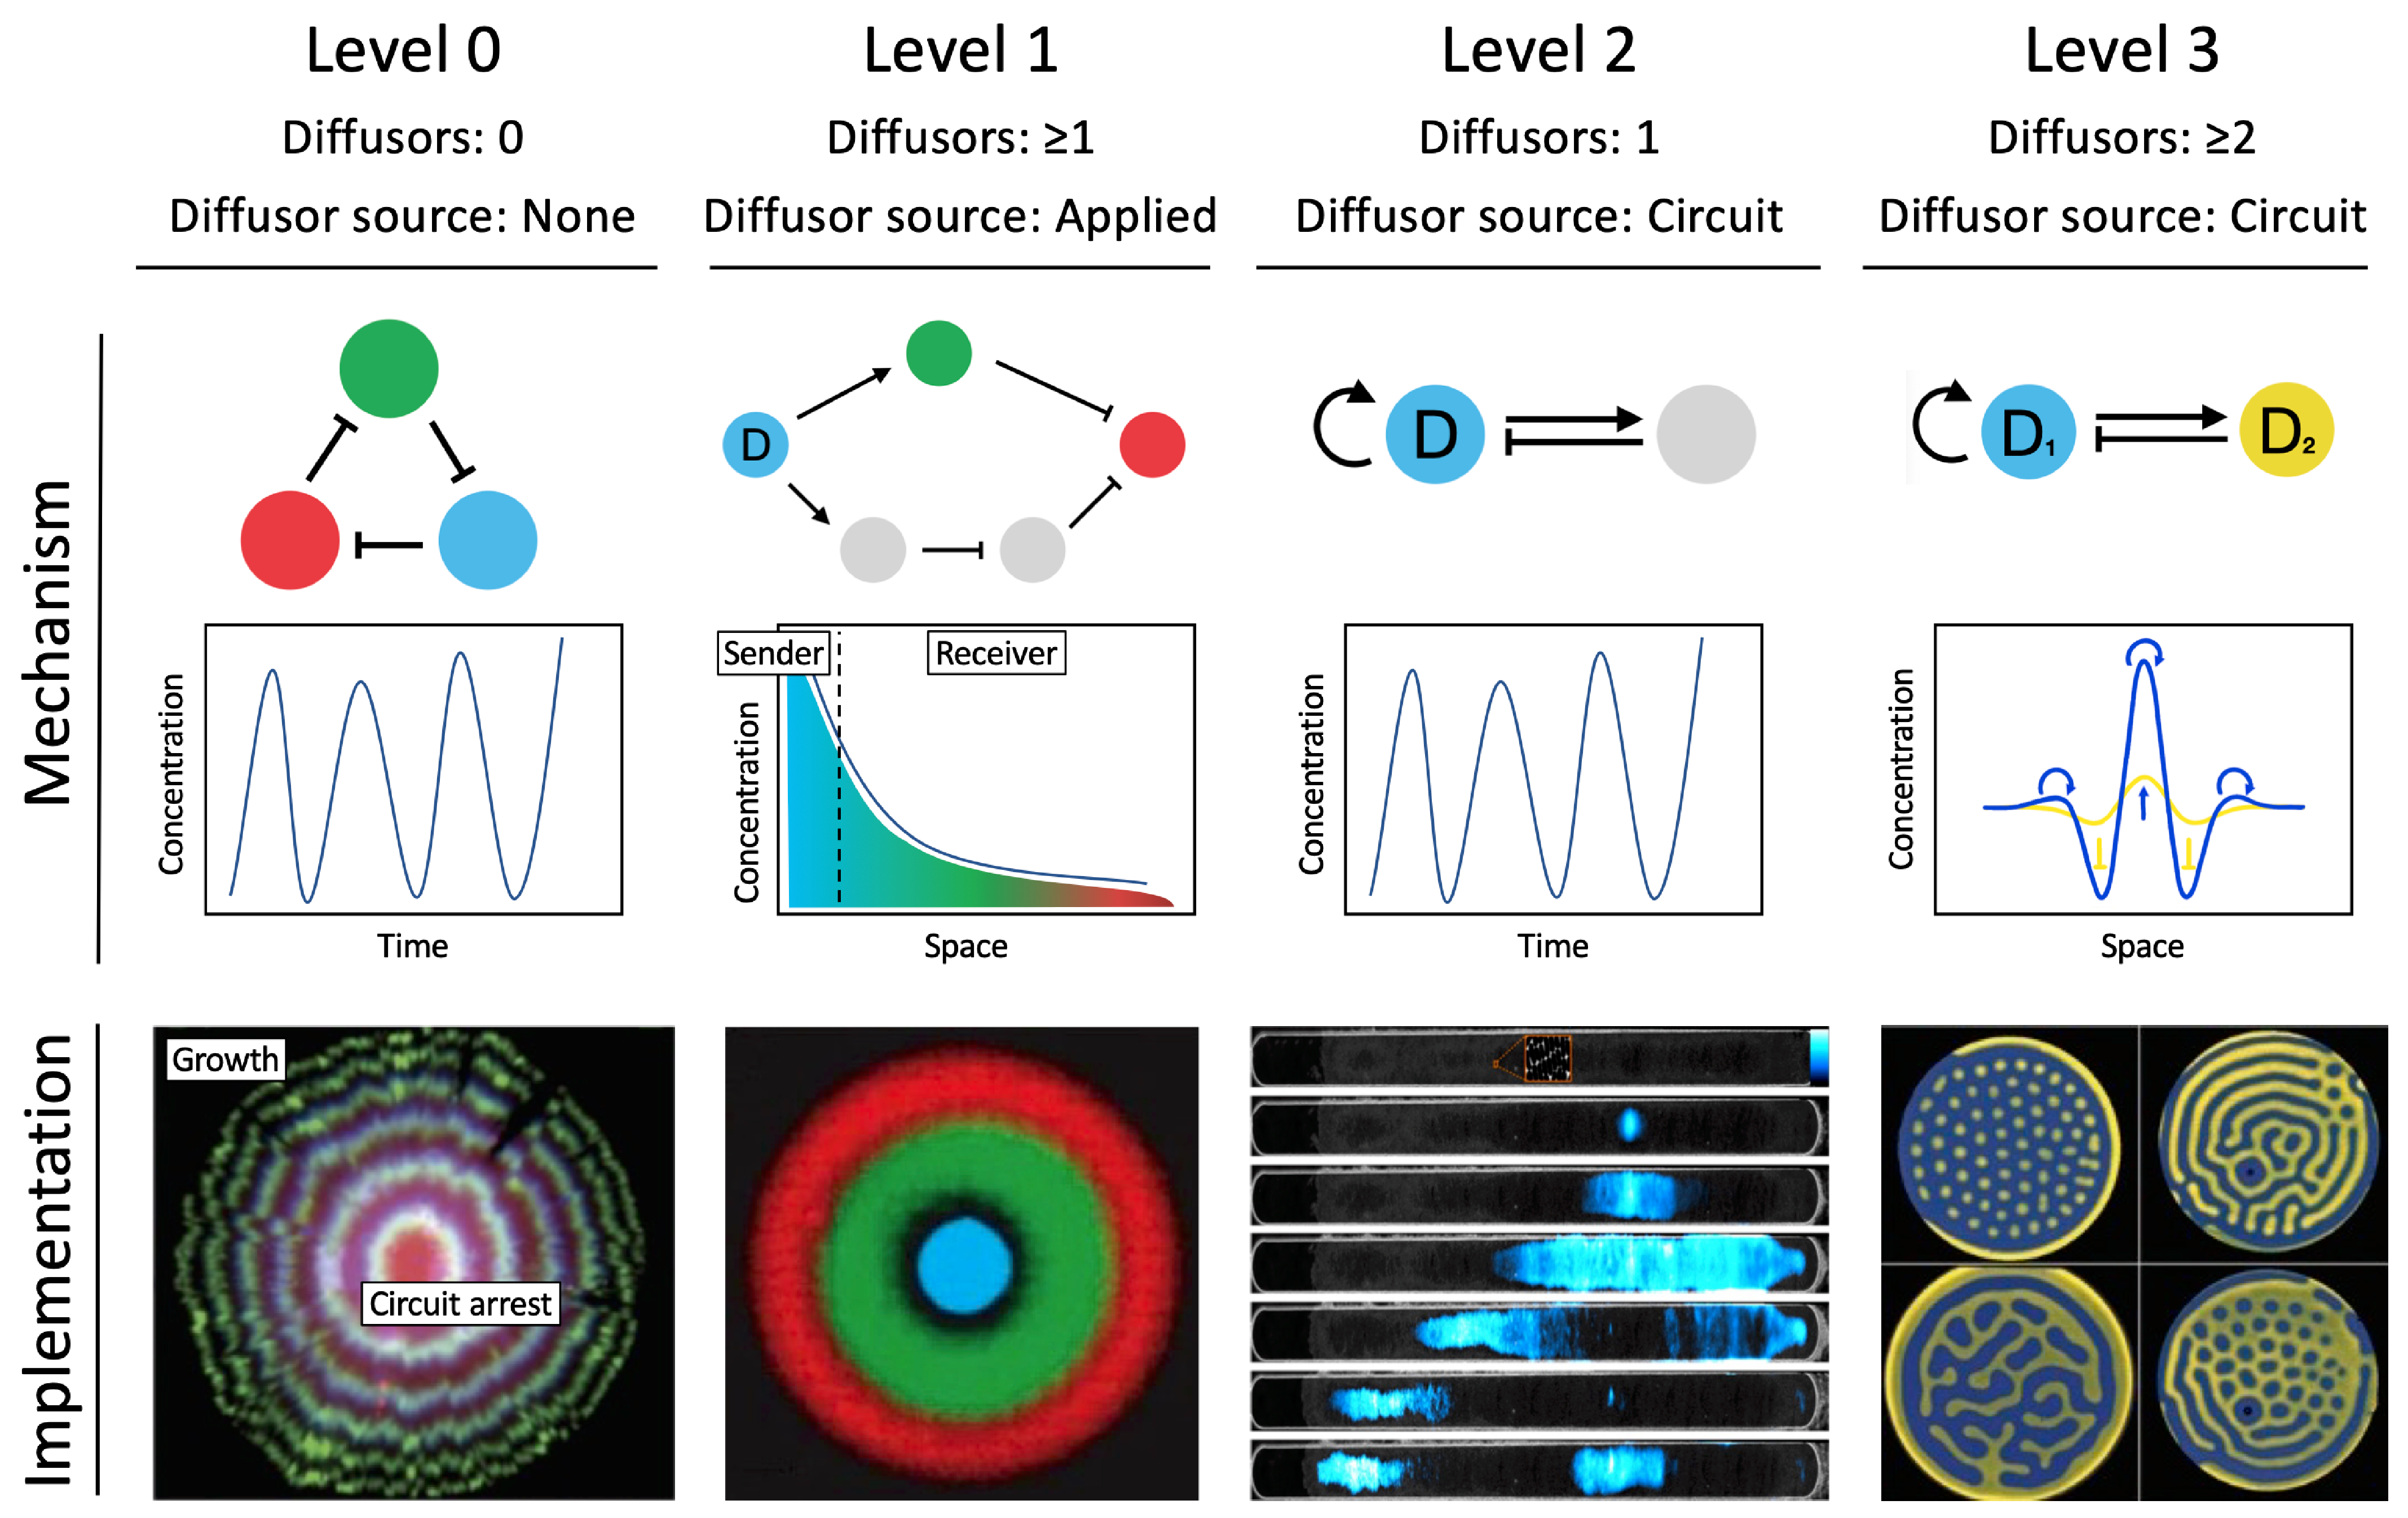
\includegraphics[width=1\textwidth]{chapters/Introduction/SpatialComponentsFigure1_300dpi}
    \caption{\textbf{Engineered spatial patterns in synthetic biology.} This figure is adapted from our published review on synthetic spatial patterning~\parencite{huidobro}. Four levels of regulatory complexity in engineered spatial patterning systems. Each level is divided into an example circuit, and the resulting pattern upon implementation. Diffusing components of the circuit are labelled with a “D”, non-diffusing nodes are unlabelled. The colour of each node corresponds to the colour of the reporter in the respective implementation. Level 0: synchronized repressilator circuit implemented in a growing bacterial colony \parencite{Potvin-Trottier2016}. The plot shows the circuit oscillations in single cells or stirred liquid culture. Level 1: incoherent feedforward circuit, where the diffusor-producing sender cells (cyan) are placed in the middle of a bacterial lawn~\parencite{Basu2005}. The plot shows the concentration gradient of the diffusor away from the centre of the lawn. Level 2: self-activation and feedback inhibition circuit with one dynamically regulated diffusor creates spatial propagating waves and spatially synchronised oscillations (not shown)~\parencite{Danino2010}. The plot shows the oscillations of the circuit in single cells, or in a cell population. Level 3: self-activation and lateral-inhibition circuit with two dynamically regulated diffusors creates stationary Turing patterns in the TuIS chemical system~\parencite{Horvath}. The plot shows the localized, self-activating positive feedback of the slow-diffusing species D1 (blue curve) and the lateral inhibition of the fast-diffusing species D2 (yellow curve).} %TODO comment on adapted from literature
    \label{fig:engineered_patterns}
\end{figure}

Level 0 circuits lack synthetic signals that diffuse through normal Fickian diffusion, where the molar flux due to diffusion is proportional to the concentration gradient.
Instead, spatial structures emerge from other processes like cellular growth and gene expression freezing.
Examples include synchronised oscillator circuits in bacterial colonies producing periodic concentric ring patterns without diffusing signals~\parencite{Potvin-Trottier2016, Riglar2019} (See Fig.~\ref{fig:engineered_patterns} Level 0).

Level 1 circuits do rely on diffusible components; however, these are not dynamically regulated, meaning they are not produced by the circuit as it is in the case of Turing patterns.
These diffusors only act as a pre-pattern which the system will interpret~\parencite{Basu2005, Schaerli2014, Kong2017, Barbier2020, Grant2020}.
Although stripes and sharp boundaries can be obtained, their periodicity is limited.
Hierarchical patterning circumvents the periodicity issue by increasing the number of orthogonal diffusors used, which linearly increases the number of spatial domains~\parencite{Boehm2018}.
While hierarchical patterns can explain some developmental periodic patterns such as the neural tube in vertebrates~\parencite{Briscoe2015}, it fails to capture the self-organising periodicity of Turing patterns observed in development such as digit patterning~\parencite{Sheth2012,Raspopovic1} (see Fig. \ref{fig:engineered_patterns} Level 1).

Level 2 circuits do incorporate dynamically regulated diffusors; however, only one diffusor is introduced.
In contrast with level 1 systems, no pre-patterns are required to generate interesting behaviours.
Starting from a spatially homogeneous regime, these systems can produce robust spatial oscillators such as~\parencite{Danino2010} or simple single ring patterns~\parencite{Cao2016, Payne2013} (see Fig. \ref{fig:engineered_patterns} L evel 2).

Finally, level 3 circuits use multiple dynamically regulated diffusible components (see Fig.\ref{fig:engineered_patterns} Level 3).
Turing patterns are the most prominent example of Level 3 systems as they as formed by reaction-diffusion circuits of at least two diffusors.
While numerous robust systems have been engineered in Level 0,1 and 2 circuits, Level 3 or Turing pattern engineering are still in its infancy.
Stochastic Turing patterns were recently engineered in \textit{E.~coli} with a circuit implemented according to the self-activation and lateral inhibition topology, with two diffusible quorum-sensing signals~\parencite{Karig2018}.
Additionally, solitary patterns have also been engineered in a refactored Nodal–Lefty system in HEK cells~\parencite{Sekine2018}.
While easier to engineer due to their relaxed fine-tuning requirements, stochastic Turing patterns and solitary display more irregularity in their periodic spatial structure~\parencite{Butler2011, Karig2018,Sekine2018}.
x
While elusive in synthetic biology, regular-repeat Turing patterns have been engineered in chemical reaction systems.
They were first observed in the 1990's in the chlorite-iodide malonic acid (CIMA) reaction~\parencite{Castets, Lengyel1992} and later in the thiourea-iodate-sulfite (TuIS) reaction~\parencite{Horvath} (see Fig. \ref{fig:engineered_patterns} Level 3).
Unlike biological systems, chemical reactions are reliably described by the simpler laws of mass action, and system parameters can often be identified~\parencite{turanyi1994, kugler2009, Pusnik2019, Yeoh2019}.
Furthermore, the tuning of these systems by changing initial concentration or temperature has more predictable effects on the system~\parencite{Horvath, landeira2010, Asakura2011}.
Lastly, chemical systems are isolated from external interacting components unlike biological systems where burden and cross-talk between the cellular chassis and synthetic parts is inevitable~\parencite{Ceroni2015, Nielsen2016,Butzin2018, Du2020}.


Although chemical systems have helped understand pattern formation and could prove key to tissue engineering applications, mechanisms in biology seem to go beyond chemical systems.
Examples of patterns have been closely linked to gene expression patterns as shown in \textit{in-situ} hybridization studies~\parencite{Jing2006}.
For this reason, it is key to explore this avenue and build genetically based reaction-diffusion systems that generate robust periodic patterns in biofilms.


%todo comment that patterns are linked to gene expression because Modern experimental interrogations of suspected mor-phogen-based pattern formation systems, such as Nodal and Lefty zebrafish mesendodermal induction,use in situ hybridization [24–26]. This explicitly highlights local concentrations of specific mRNA tran- scripts and thus provides an indication of the rates of transcription of target genes, and emphasizes the role of gene expression in morphogenesis. Chen, Y. & Schier, A. F. 2002 Lefty proteins are long-
%range inhibitors of squint-mediated nodal signaling. Curr.
%Biol. 12, 2124–2128. (doi:10.1016/S0960-9822(02)01362-3)
%25 Jing, X. H., Zhou, S. M., Wang, W. Q. & Chen, Y. 2006
%Mechanisms underlying long- and short-range nodal
%signaling in Zebrafish. Mech. Dev. 123, 388–394.
%(doi:10.1016/j.mod.2006.03.006)
\subsection{Engineering Turing patterns in bacterial biofilms using exogenous circuit}
Even though they have been successfully engineered in chemical systems, the complexity of biology means that Turing patterns have never been engineered in a genetic context.
This can be attributed to the robustness problem including high sensitivity of parameters and a small fraction of parameter space producing Turing solutions.
Additionally, designing Turing circuits with the classical 2-node topology leads to constraints in differential diffusivity that hinder the engineering of Turing patterns.
Finally, this robustness issue is further amplified by the lack of orthogonal small-diffusible regulators to act as morphogens in a synthetic reaction-diffusion circuit.
Orthogonality refers to the inability of two or more molecules to interact with their respective substrates, so the activator or inhibitor functions work adequately.
%
%All these issues have been addressed by previous researchers in the Isalan Lab and myself to achieve the engineering of a synthetic Turing circuit in bacteria that can produce regular periodic stationary patterns.

To address the fine-tuning problem and differential diffusivity constraints,~\cite{Scholes2019} found that topology \#3954 was amongst the most robust 3-node networks in terms of kinetic parameters. %TODO ref topology if image is included
Additionally, this topology allowed for equal diffusivity and even faster diffusing activators.
A search around neighbours of the \#3954 topology was carried out to find that removing the positive feedback on node A did not decrease robustness substantially.
The resulting \#1754 topology seemed like a better candidate as it would be easier to build experimentally, while maintaining the robustness.
This topology is shown in Fig.~\ref{fig:synthetic circuit} (grey inset)

The lack of robust biological partly was addressed in~\cite{Meyer2019} and~\cite{Du2020} where orthogonal morphogens where characterized, which allow the building of the \#1754 topology.
These orthogonal morphogens are small quorum-sensing molecules which can activate gene expression by binding a promoter with high specificity, to activate downstream gene expression.
These toolboxes are key to bridge the gap between abstract models and real-sender receiver circuits.
Additionally, in~\cite{huidobro} we compiled a list of small molecule regulators that can diffuse and form gene circuits in \textit{E.~coli}, as well as their respective promoters and synthesis enzymes.
These could be investigated in the future to use as additional morphogens to build more complex systems with more diffusible molecules.

Finally,~\cite{Tica2020} engineered the \#1754 topology using the components from~\cite{Meyer2019} and~\cite{Du2020}, with the aim of exploring a Turing gene circuit for pattern formation (see Fig.~\ref{fig:synthetic circuit} bottom).
Due to the lack of specific biological parts such as an inhibitor quorum sensing molecule or a dual inhibitor/activator molecule, the biological implementation of \#1754 resulted in a six molecular species circuit instead of the original 3-node network.

\begin{figure}[H]
    \centering
    \includegraphics[width=1\textwidth]{chapters/Chapter 2/synthetic circuit2}
    \caption{\textbf{Synthetic biology implementation of \#1754 topology.} This synthetic circuit engineered by Jure Tica and Tong Zhu is a genetic abstraction of the \#1754 topology in \cite{Scholes2019}. This circuit is transformed so every \textit{E.~coli} cell in the biofilm has a copy inside. The original topology (left, grey inset) has only three nodes, while the synthetic circuit (right) has 6 nodes. The 6 gene circuit architecture, s hown in standard notation, can be clustered into the three original nodes as seen by the blue,green,red bubbles. Diffusor synthesis enzymes are in blue, non-diffusible transcription
    factors in red, fluorescent proteins in white. Diffusor synthesis enzymes produce quorum sensing molecules $pC$ and $OC_{14}$. The circuit can be regulated by small molecules ATC, IPTG and DAPG shown in white bubbles. DAPG activates the control cassette produces regulated degradation of small quorum sensing molecules. The bottom cassette (orange), contains the neccesary regulators: RpaR is the pC receptor (Node A diffusor), CinR is the OC14 receptor (Node B diffusor), and PhlF is the DAPG receptor (used to tune inducible diffusor degradation). The other three receptors PcaU, NahR and VanR are for the protocatechuate, salicylate and vanillin inducers, which are not used in the present circuit, but were tested in other versions of the system. These three systems can be used to introduce additional regulatory components to the system.}
    \label{fig:synthetic circuit}
\end{figure}

In this thesis, theoretical work based on this synthetic gene circuit was carried out to understand how to tune parameters experimentally and what spatial setup to use to allow pattern formation in bacterial biofilms.
Additionally, once the setup is determined, to predict which patterns might appear and the relevant wavelengths to look for.
Finally, once patterns appear in the biofilm, to characterise and understand the mechanisms behind these patterns.

Having a genetic synthetic network that produces patterns with a predictive model would be extremely impactful on various levels.
Firstly, the model would allow us to understand the patterning mechanisms behind the synthetic system and therefore shed some light into developmental biology.
Currently, our understanding from top-down approaches is based on arbitrarily chosen models that match well the experiments, but that are not directly informed on well-known and characterised gene circuits.
Model selection from those experiments is practically impossible as it has been proven that different models can generate the same 1D or 2D Turing pattern~\parencite{Woolley2021}.
In this bottom-up approach, the model used is derived from a known synthetic gene circuit that has been artificially introduced into cells.
This process constraints the model to provide more insightful results.
If this network can produce self-assembling periodic stationary patterns both~\textit{in-silico} and~\textit{in-vitro}, it would prove that a known reaction-diffusion system supported by genetic interactions can produce Turing patterns, therefore validating this mechanism.
Secondly, having a model would allow us to inform the experimentalists on how to tune the system to obtain more robust desired patterns or different shapes for tissue engineering in biotechnology applications.


\section{Thesis overview}

%%TODO mention chapter 1 and chapter 2 are a paper

This thesis explores Turing patterning within synthetic biology and tissue engineering, employing a modeling approach.
The novelty of this thesis lies in its modeling aspects, although it also includes some experimental results.

The first chapter adopts a theoretical perspective, delving into the relationship between linear stability analysis and numerical solutions.
Key aspects include estimating wavelength, convergence time, and, in some cases, predicting pattern shapes from the dispersion relation.
It also examines various instabilities capable of producing stationary spatial patterns beyond classical Turing instabilities.
This theoretical framework sets the stage for addressing realistic biological phenomena in pattern formation, such as varying boundary conditions and growth, crucial for understanding and engineering synthetic gene circuits for pattern formation.

The second chapter aims to develop a predictive model for the \#1754 topology, informed by the synthetic gene circuit outlined in~\cite{Tica2020}.
This PDE model is based on the interactions between genetic components and the diffusion of quorum-sensing molecules.
This model is used to explore the system's parameter space to identify regions prone to robust pattern formation and strategies for experimental tuning of the gene circuit.
Additionally, the model is parameterized using liquid culture data to determine its position within the parameter space.

The final chapter focuses on the experimental and modeling aspects of synthetic biofilms and their emergent patterns.
It presents initial experiments on small colonies forming periodic rings.
A PDE solver, combined with a cellular automaton for modeling bacterial colony growth, is then introduced, replicating all observed patterns, including spots, wedges, and rings produced by collaborators.
The chapter concludes with a detailed examination of the model's predictability against experimental perturbations, emphasizing the analysis of irregular growth, boundary effects, and node deletions.

In conclusion, this thesis significantly contributes to the fields of biology and mathematical biology, particularly in the realm of synthetic patterning.
By employing a predictive model and optimizing robustness, this work demonstrates the ability to guide experimental design for pattern formation as well as replicating the complex patterns obtained.
However, despite these advancements, the current level of robustness achieved remains relatively low, highlighting the need for further research.
Future work should focus on deepening our understanding of the underlying mechanisms and refining techniques to enhance the robustness and reliability of synthetic patterning processes.
This will be crucial in realizing the full potential of this technology in biomedical and industrial applications.


    \chapter{Beyond classical Turing patterns}\label{Chapter 1}
\section{Synopsis}
The Turing instability is a well-known mechanism for pattern formation. Turing instabilities are defined and studied using \acrfull{LSA}, but they can also be further explored with numerical methods. LSA predicts whether a pattern will occur through the dispersion relation, where the real part of eigenvalues determines the system's stability as a function of a wavenumber parameter. Although fast, this method provides limited insight into the emerging pattern, as it relies on linearization around the steady state. On the other hand, numerical methods, while more computationally intensive, offer detailed results of the developing pattern, including the concentration of species over time and space. Numerical results also enable visualization of the resulting Turing pattern shape, which in 2D can consist of spots, stripes, or labyrinths

To effectively conduct a high-throughput study exploring the \#1754 synthetic Turing gene circuit built in~\cite{Tica2020}, it is essential to leverage LSA.
LSA offers a much quicker alternative compared to numerical methods for understanding the patterning capabilities of the experimental circuit.
However, LSA, which relies on linearization around the steady state, sometimes fails to predict pattern formation accurately.
Understanding what information can be obtained from LSA before resorting to numerical methods, and when LSA predictions break, will enable us to efficiently gather extensive insights into both the patterning potential and the robustness of the system.

In this chapter, we first study the relationship between the analytical dispersion relation and the numerical results in Turing patterns.
This includes understanding how to predict wavelength,
convergence time and even pattern shape from the dispersion relation.
This is important to obtain information from the emergent pattern without having to solve the \acrfull{PDE} numerically.
Then we explore how LSA might not always be a good predictor of pattern formation.
For example, how multistability can break LSA predictions and how other types of dispersion relation profiles or instabilities which are not classical Turing can generate stationary spatial patterns or other types of temporal-spatial patterns.
Finally, we explore numerically how these patterns behave when realistic biological features present in our experimental setup are introduced, such as absorbing boundaries or growth.



\section{Linear stability analysis and the dispersion relation}\label{lsa}
\subsection{Linear stability analysis for a reaction-diffusion system}


The following section describes how LSA is carried out for the steady states in a reaction-diffusion system.
This analysis aims to find out if the steady state exhibits a Turing instability which is also called a diffusion-driven instability.
When it does, the system is capable of forming spatial patterns.
As the name describes, diffusion-driven instabilities arise in these systems when a homogeneous steady state is stable to small perturbations in the absence of diffusion, and becomes unstable in the presence of diffusion~\parencite{Glendinning1994, J.DMurray2002}.
To check for Turing instabilities, the stability of the equilibrium state will be studied without and with diffusion.
The method of LSA will be explained for the two morphogen reaction-diffusion system, shown below:


\begin{subequations}
    \begin{equation}
        \pdv{A}{t}= f_{A}(A, I) + D_{A}\nabla^2 A
        \label{eq:RD general equation 1}
    \end{equation}
    \begin{equation}
        \pdv{I}{t} = f_{I}(A, I) + D_{I}\nabla^2 I
        \label{eq:RD general equation 2}
    \end{equation}
    \label{eq: RD general equations}
\end{subequations}
where $f_{A,I}$ are the non-linear production terms and $D_{A,I}$ are the diffusion constants of the two morphogens.

\subsubsection{Stability of steady state without diffusion}
To study the stability around the steady state without diffusion, only the reaction terms of Eqs.\ref{eq: RD general equations} are used:
\begin{subequations}
    \begin{equation}
        \pdv{A}{t} = f_{A}(A,I)
    \end{equation}
    \begin{equation}
        \pdv{I}{t} = f_{I}(A,I)
    \end{equation}
    \label{eq: R general equations}
\end{subequations}
There is no space dependence here as diffusion terms have been removed.
Therefore, there is only time dependence.
The steady states are defined as $A^*$ and $I^*$, which satisfy the condition:
\begin{equation}
    f_{A}(A^*,I^*)=0, \hspace{1.5cm} f_{I}(A^*,I^*)=0
\end{equation}
In this section, X is a vector with the two morphogens $X=[A,I]$.
LSA is carried by adding an infinitesimally small perturbation $\delta X$ to the steady state $X^*$, and studying if the perturbation decays (stable steady state) or grows (unstable steady state) over time.
 The perturbation needs to be almost insignificant as Taylor expansion is carried out to linearise the system around the steady state. Therefore, the morphogen concentration can be expressed as:
\begin{subequations}
    \begin{equation}
        A(t) = A^* + \delta A(t),\hspace{1.5cm} |\delta A| \ll A^*
    \end{equation}
    \begin{equation}
        I(t) = I^* + \delta I(t), \hspace{1.5cm} |\delta I| \ll I^*
    \end{equation}
    \label{eq: steady states}
\end{subequations}
The differential Eqs. \ref{eq: R general equations} are evaluated at steady state, using Eqs~\ref{eq: steady states}:
\begin{subequations}
    \begin{equation}
        \pdv{A}{t} = \pdv{[A^* + \delta A(t)]}{t} = f_{A}(A^* + \delta A(t), I^* + \delta I(t)) = \pdv{\delta A}{t}
    \end{equation}
    \begin{equation}
        \pdv{I}{t} = \pdv{[I^* + \delta I(t)]}{t} = f_{I}(A^* + \delta A(t), I^* + \delta I(t)) = \pdv{\delta I}{t}
    \end{equation}
    \label{eq: R equations at steady state}
\end{subequations}
As previously mentioned, the non-linear system will be linearised around the steady state using Taylor expansion.
This is done to have a simpler set of equations, that represent the system around the steady state, as seen below:
\begin{equation}
    \begin{split}
         f(A^*+\delta A, I^*+\delta I) =  f(A^*,I^*) + \pdv{f(A^*,I^*)}{A}\delta A + \pdv{f(A^*,I^*)}{I}\delta I + \dots  \\\\ + \frac{1}{n!} \pdvn{n}{f(A^*,I^*)}{A}\delta A^n + \frac{1}{n!} \pdvn{n}{f(A^*,I^*)}{I}\delta I^n
    \end{split}
\end{equation}



%\begin{split}
%    \pdv{[X(x,t)]}{x}) = \mathcal{F}^{-1}\left(\pdv{[X(k,t)]}{x}\right) = \frac{\partial}{\partial x}\left[\frac{1}{2\pi}\int_{-\infty}^{\infty} X(k,t)e^{ikx} dk\right] =  \frac{1}{2\pi}\int_{-\infty}^{\infty} X(k,t)\frac{d}{dx}e^{ikx} dk\\\\ =\frac{1}{2\pi}\int_{-\infty}^{\infty} ik X(k,t)e^{ikx} dk = ik \frac{1}{2\pi}\int_{-\infty}^{\infty} X(k,t)e^{ikx} dk = ik X(x,t)
%\end{split}




If $\delta A$ and $\delta I$ are small enough, higher order terms in the Taylor expansion can be neglected as $\delta (A,I)^n$  becomes infinitesimally small.
This simplification is justified under the Hartman-Grobman theorem, which states that the behavior of a dynamical system near a hyperbolic equilibrium point (i.e where no eigenvalue of the linearized system's Jacobian has its real part equal to zero) is qualitatively the same as the behavior of its linear approximation.
Therefore, as long as the system's equilibrium point meets this hyperbolic condition, the linearized model provides a valid approximation for understanding the system's local dynamics.
Furthermore, by construction $f(A^*,I^*) = 0$, therefore the following expression is obtained, where $f$ corresponds to either $f_{A}$ or $f_{I}$  :
\begin{equation}
    f(A^*+\delta A, I^*+\delta I) =  \pdv{f(A^*,I^*)}{A}\delta A + \pdv{f(A^*,I^*)}{I}\delta I
\end{equation}
Finally, because $\pdv{X}{t} =  \pdv{\delta X}{t}$  at steady state (Eqs. \ref{eq: R equations at steady state}), the change in perturbation, meaning decay or growth, can be expressed as:
\begin{subequations}
    \begin{equation}
        \pdv{\delta A}{t} = \pdv{f_{A}(A^*,I^*)}{A}\delta A + \pdv{f_{A}(A^*,I^*)}{I}\delta I
    \end{equation}
    \begin{equation}
        \pdv{\delta I}{t} = \pdv{f_{I}(A^*,I^*)}{A}\delta A + \pdv{f_{I}(A^*,I^*)}{I}\delta I
    \end{equation}
    \label{eq: linearised terms around steady state}
\end{subequations}

The existence and uniqueness of the solution are guaranteed by Picard's theorem.
Here, the solution can be explicitly expressed in terms of exponential functions, where  $\sigma$ determines the growth rate of the perturbation, and whether it grows (unstable steady state) or decays (stable steady state):
\begin{subequations}
    \begin{equation}
        \delta A = A_{0}e^{\sigma t}
    \end{equation}
    \begin{equation}
        \delta I = I_{0}e^{\sigma t}
    \end{equation}
    \label{eq: exponential R}

\end{subequations}
If Eq. \ref{eq: exponential R} are introduced into Eq. \ref{eq: linearised terms around steady state}, and the solution divided by $e^{\sigma t}$ on both sides, the following is obtained:
\begin{subequations}
    \begin{equation}
        \sigma \delta A_{0} = \pdv{f_{A}(A,I)}{A} \delta A_{0} + \pdv{f_{A}(A,I)}{I}\delta I_{0}
    \end{equation}
    \begin{equation}
        \sigma \delta I_{0} = \pdv{f_{I}(A,I)}{A} \delta A_{0}+ \pdv{f_{I}(A,I)}{I}\delta I_{0}
    \end{equation}
\end{subequations}
If the Jacobian J of this system is
\begin{equation}
    J = \begin{bmatrix}
            \pdv{f_{A}}{A} &
            \pdv{f_{A}}{I}  \\
            \pdv{f_{I}}{A} &
            \pdv{f_{I}}{I}
    \end{bmatrix}
\end{equation}
This can be represented as an eigenvalue-eigenvector problem using the jacobian $J$, the eigenvalue $\sigma$ and the eigenvector  $\delta X_{0} = [\delta A_{0},\delta I_{0}]$:
\begin{equation}
    \sigma \cdot \delta X_{0} = J \cdot \delta X_{0}
\end{equation}
Finally, $\sigma$ can be obtained by solving the characteristic polynomial:
\begin{equation}
    p(\sigma) = det[J-\sigma I] = 0
\end{equation}


For a system with two variables, there are two eigenvalues $\sigma_{1}$ and $\sigma_{2}$.
The real part of $\sigma$ corresponds to the growth rate of the perturbation.
$Im(\sigma)$ corresponds to the oscillations.
If all $Re(\sigma) < 0 $, the steady state will be stable to perturbations, which means the system will go back to the steady state after a small perturbation is applied.
If at least one $Re(\sigma) > 0 $, the steady state will be unstable to perturbations, and the system will go away from the equilibrium point after being slightly perturbed.
The first requirement for a Turing instability is that the system without diffusion is stable, therefore all eigenvalues must have a negative real part.



\subsubsection{Stability of steady state with diffusion}
Once the stability of the steady state has been analysed in the absence of diffusion, the effect of diffusion on the same system will be studied.
The diffusion will be introduced through the partial derivative term $D_{X}\nabla^2 X$.




\paragraph{Definition of a function in a finite system with no-flux boundary conditions:}
A function X(x), which represents the concentration of molecule X in space x, is defined in a finite-domain [0,L] with no-flux boundary conditions.
No-flux boundary conditions imply that the derivative of the function at the boundaries is zero:

\begin{equation}
    \frac{\partial X}{\partial x}\Bigg|_{x=0} = \frac{\partial X}{\partial x}\Bigg|_{x=L} = 0
\end{equation}


A general Fourier series representation of X(x) under these conditions can be:

\begin{equation}
    X(x) = \sum_{n=0}^{\infty} \left( A_n \cos\left(\frac{n \pi x}{L}\right) + B_n \sin\left(\frac{n \pi x}{L}\right) \right)
\end{equation}

However, because the derivative at the boundary is zero, the cosine series is used instead.
This is because the derivative of $\cos(0)$ or $\cos(n\pi)$ is zero.
Therefore, the Fourier cosine series used is

\begin{equation}
    X(x) = \sum_{n=0}^{\infty}  C_n \cos\left(\frac{n \pi x}{L}\right)
    \label{cosine_series}
\end{equation}

This way, if the function X(x) is expressed in terms of cosines (see Fig.~\ref{fig:cos_boundary_conditions}), the derivatives of this function for $x=0$ and $x=L$ are zero:
\begin{equation}
    \frac{\partial \left(cos(0)\right)}{\partial x} = 0 ; \quad \frac{\partial \left(cos(\frac{n \pi L}{L})\right)}{\partial x} = 0
    \end{equation}

\begin{figure}[H] % h! is a placement specifier; it tries to place the image here.
    \centering
    \includegraphics[width=0.8\textwidth]{chapters/Chapter 1/cos_boundary_conditions} % The name of your image file; assumes it is in the same directory as your .tex file
    \caption{\textbf{No-flux boundary conditions represented with cosine wave}}
    \label{fig:cos_boundary_conditions} % A label for referencing this figure later in the document
\end{figure}

\paragraph{Derivative of function in space:}
The Laplacian Operator $\nabla^2$ is applied to X(x) to represent the diffusion terms
\begin{equation}
    \nabla^2 X(x) = \frac{\partial^2}{\partial x^2} \left(\sum_{n=0}^{\infty}  C_n \cos\left(\frac{n \pi x}{L}\right) \right)  = - \sum_{n=0}^{\infty}  C_n \left(\frac{n \pi }{L}\right)^2 \cos\left(\frac{n \pi x}{L}\right)
\end{equation}

If we replace the original cosine series expressing X(x) (Eg.~\ref{cosine_series}) into this equation, we obtain
\begin{equation}
    \nabla^2 X(x) = -\left(\frac{n \pi }{L}\right)^2 X(x)
\end{equation}


\paragraph{Wavenumber definition:}
The wavenumber $k$ is the spatial frequency of the wave, measured in cycles or radians per unit distance.
In this case, the wave X(x) is expressed in cosine form.
As previously explained, to satisfy the no-flux boundary conditions, the derivative of this cosine must be zero at the boundaries $x=[0,L]$.
Therefore, $k_{n}$ must be
\begin{equation}
    k_{n}=\frac{n \pi}{L}
\end{equation}

Once $k_{n}$ is defined for our boundary conditions, the expression for the Laplacian becomes

\begin{equation}
    \nabla^2 X(x) = - k_{n}^2  X(x)
    \label{eq: simplified fourier diffusion}
\end{equation}



\paragraph{Linear stability analysis of steady state with diffusion effects:}
Now that the PDE diffusion term has been reduced to an ODE term, and the zero-flux boundary conditions introduced, the stability of the steady state when introducing diffusion can be studied.
As shown in Eqs.~\ref{eq: simplified fourier diffusion}, the diffusion term $\nabla^2 X(x)$ can be expressed as $- k_{n}^2  X(x)$, therefore the linearised reaction-diffusion PDE equations can be written as
\begin{subequations}
    \begin{equation}
        \pdv{A}{t} = f_{A}(A^*+\delta A, I^*+\delta I)  -D_{A}k_{n}^2A
    \end{equation}
    \begin{equation}
        \pdv{I}{t} = f_I(A^*+\delta A, I^*+\delta I) -D_{I}k_{n}^2I
    \end{equation}
\end{subequations}
where $k_{n}=\frac{n\pi}{L} \hspace{0.1cm}\forall n \in \{0, \mathbb{N}\} $.

In the previous section, LSA was carried around the steady state with a perturbation $\delta X$, without including diffusion.
This resulted in the expression shown in Eq.~\ref{eq: linearised terms around steady state}, which describes the linearized reaction terms around the steady state.
By adding diffusion in the Fourier domain from Eq.~\ref{eq: simplified fourier diffusion} we obtain the following expression for the linearized reaction-diffusion system, where A and I are now a function of $k_{n}$ and $t$:

\begin{subequations}
    \begin{equation}
        \pdv{\delta A}{t} = \pdv{f_{A}(A^*,I^*)}{A}\delta A + \pdv{f_{A}(A^*,I^*)}{I}\delta I  -D_{A}k_{n}^2\delta A
    \end{equation}
    \begin{equation}
        \pdv{\delta I}{t} =  \pdv{f_{I}(A^*,I^*)}{A}\delta A + \pdv{f_{I}(A^*,I^*)}{I}\delta I  -D_{I}k_{n}^2\delta I
    \end{equation}
    \label{eq:linearised RD}
\end{subequations}

We wish to find a general solution of the form:

\begin{subequations}
    \begin{equation}
        \delta A = A_{0}e^{\sigma t}\cdot e^{ik_{n}x}
    \end{equation}
    \begin{equation}
        \delta I = I_{0}e^{\sigma t}\cdot e^{ik_{n}x}
    \end{equation}
    \label{eq: exponential form RD}
\end{subequations}
where $X_{0}e^{\sigma t}$ represents the amplitude of the perturbations and $e^{ik_{n}x}$ represents the spatial oscillations (with $k_{n}$ as the wavenumber).
In this case, we are interested on the growth or decay of the perturbations over time.
Therefore, to observe the stability of the steady state, we will study the amplitude term ($X_{0}e^{\sigma t}$):
\begin{itemize}
    \item If $\sigma > 0$: perturbation ($\delta X$) grows making $\pdv{\delta X}{t} > 0$.
    Therefore, the steady state is unstable with diffusion.
    \item If $\sigma < 0$: perturbation ($\delta X$) decays making $\pdv{\delta X}{t} < 0$.
    Therefore, the steady state is stable with diffusion.
\end{itemize}
If Eqs.~\ref{eq: exponential form RD} are substituted into Eqs.~\ref{eq:linearised RD}, the following equations are obtained:
\begin{subequations}
    \begin{equation}
        \sigma \delta A_{0} = \pdv{f_{A}(A^*,I^*)}{A} \delta  A_{0}  + \pdv{f_{A}(A^*,I^*)}{I}\delta  I_{0} -D_{A}k_{n}^2\delta  A_{0}
    \end{equation}
    \begin{equation}
        \sigma \delta I_{0}= \pdv{f_{I}(A^*,I^*)}{A} \delta  A_{0}  + \pdv{f_{I}(A^*,I^*)}{I}\delta  I_{0}  -D_{I}k_{n}^2\delta A
    \end{equation}

\end{subequations}
If the Jacobian J of this system is
\begin{equation}
    J = \begin{bmatrix}
            \pdv{f_{A}}{A} - D_{A}k_{n}^2 &
            \pdv{f_{A}}{I}  \\
            \pdv{f_{I}}{A} &
            \pdv{f_{I}}{I} - D_{I}k_{n}^2
    \end{bmatrix}
    \label{jacobian_diffusion}
\end{equation}

these pair of equations can again be treated as an eigenvalue-eigenvector problem written in the following way:
\begin{equation}
    \sigma \cdot\delta X_{0} = J \cdot\delta X_{0}
    \label{eq: jacobian RD}
\end{equation}
where $\sigma$ can be obtained by solving the characteristic polynomial:
\begin{equation}
    p(\sigma) = det[J-\sigma I] = 0
    \label{eq: characteristic polynomial RD}
\end{equation}
In summary, to understand if perturbations around the steady state decay or grow when diffusion is introduced, Eq.~\ref{eq: characteristic polynomial RD} must be solved to obtain $\sigma$.
This characteristic polynomial is solved for a range of k's, being $k_{n}=\frac{n\pi}{L} \hspace{0.1cm}\forall n \in \{0, \mathbb{N}\} $.
The sign of $\sigma$ is studied for every $k_{n}$, resulting in the dispersion relation (Fig.~\ref{fig:turing_vs_noturing}).
If $\sigma > 0$, perturbations grow around the steady state and the system is unstable.
On the contrary, if  $\sigma < 0$, the system is stable and perturbations decay around the steady state.
More detail on LSA can be found in~\cite{J.DMurray2002} or~\cite{Glendinning1994}.

\subsubsection{Linear stability analysis implementation}
LSA is carried out with and without diffusion for all steady states of the system found using the Newton-Raphson method (see Section~\ref{newton_raphson}).
The analysis is done for all $k_{n}=\frac{n\pi}{L} \hspace{0.1cm}\forall \{n \in \mathbb{N} : n \leq 5000\} $, meaning 5000 k's are sampled using linear stability analysis.
L is defined as 100mm which is based on the maximum length of our experimental system, described in Chapter~\ref{chapter3}.
LSA for a single steady state takes approximately approximately 0.5s.

\subsection{Model definition and database creation}
The system studied in this chapter consists of a 2-node Turing topology system with non-linear Hill terms.
The activator A activates itself and I, while the inhibitor I inhibits the activator A as seen in Fig.~\ref{fig:intro_to_Turing_patterns}A.
However, instead of using the linear terms used in the original Turing system Fig.~\ref{fig:intro_to_Turing_patterns}B~\parencite{Turing1952}, we use Hill terms which represent genetic regulations.
More information on how these Hill terms represent gene expression regulations can be found in Section~\ref{Protein equations and gene regulation}.

\begin{subequations}
    \begin{equation}
        \pdv{[A]}{t}=b_{A}+V_{A} \cdot\frac{1}{1+\left(\frac{K{A}}{[A]}\right)^{n_{A}}}\cdot\frac{1}{1+\left(\frac{[I]}{K_{I}}\right)^{n_{I}}}-\mu_{A}\cdot[A] + D_{A}\nabla^2 [A]
%        \pdv{[A]}{t}=b_{A}+V_{A} \cdot\frac{1}{1+\left(\frac{K{A}}{[A]}\right)^{n_{A}}}\cdot\frac{1}{1+\left(\frac{[I]}{K_{I}}\right)^{n_{I}}}-\mu_{A}\cdot[A] + D_{A}(\partial_{xx} + \partial_{yy})[A]
    \end{equation}

    \begin{equation}
        \pdv{[I]}{t}=b_{I}+V_{I} \cdot\frac{1}{1+\left(\frac{K{A}}{[A]}\right)^{n_{A}}}-\mu_{I}\cdot[I] +
        D_{I}\nabla^2 [I]
%        D_{I}(\partial_{xx} + \partial_{yy})[I]
    \end{equation}

    \label{eq:turinghill}
\end{subequations}

To study this system, the parameter space is scanned using LSA and numerical methods.
The parameter space is sampled using Latin hypercube sampling (LHS) (see Fig.~\ref{fig:distributions}A) drawn from loguniform distributions (see Fig.~\ref{fig:distributions}C).
The LHS method is designed to cover the parameter space more efficiently with fewer samples than grid or uniform sampling~\parencite{Chrisman2014, Iman2014}.
More information on sampling and distributions used can be found in the Methods Section~\ref{sampling method}.
Ranges and values used for these distributions are shown in the Appendix Tables~\ref{tab:variant_1} and~\ref{tab:variant_2}.

All results are stored in a PostgreSQL database created from scratch for this project.
This database includes interconnected tables for model parameters, numerical parameters, analytical results, numerical solutions and pattern classification outputs.
More details on the database schema can be seen in the Section~\ref{PostgreSql database}.
The creation of this PostgreSQL database was necessary to explore large parameter spaces and compare between analytical and numerical results in an efficient way.

\subsection{Diffusion-driven instabilities in the dispersion relation}
Classical Turing patterns, also called \acrfull{DDI} or Turing instabilities, can be detected using LSA as described above.
In linear stability analysis, the dispersion relation is studied, which shows the dependency of the eigenvalues $\sigma$ on the wavenumber $k_{n}$ as seen in Eq.~\ref{eq: jacobian RD}.
For a Turing instability to occur, at $k_{0}=0$, $Re(\sigma)$ must be negative, meaning the system is stable without diffusion.
As diffusion is introduced and $k_n>0$, the system becomes unstable with $Re(\sigma)>0$.
For $k_n \rightarrow \inf$, the system must be stable again and the eigenvalue negative.
This is because otherwise, a Turing II instability will occur where the dominant mode has an infinitesimally large wavenumber meaning an infinitesimally small wavelength.
The relationship between wavenumber $(k_{n})$ and wavelength $(\lambda)$ is
\begin{equation}
    \lambda_n = \frac{2 \pi}{k_n}
    \label{eq:wavelength_wavenumber}
\end{equation}

An example of a classical Turing instability with a positive dispersion peak is shown in Fig.~\ref{fig:turing_vs_noturing}B, along with the corresponding stationary spatial pattern.
Alternatively, Fig.~\ref{fig:turing_vs_noturing}A shows a spatially homogeneous solution which results from a stable system that does not exhibit a diffusion-driven instability.
These ~\acrfull{1D} numerical results were produced using the \acrfull{CN} numerical scheme described in~\ref{cranknicolson}, programmed using \textit{numpy} in Python from first math principles.
The boundary conditions used here are Neumann boundary conditions where the derivative at the boundary is zero ($\pdv{U}{x}=0$) for both molecular species, A and I.

\begin{figure}[H] % h! is a placement specifier; it tries to place the image here.
    \centering
    \includegraphics[width=01\textwidth]{chapters/Chapter 1/turing_vs_noturing} % The name of your image file; assumes it is in the same directory as your .tex file
    \caption{\textbf{The dispersion relation of reaction-diffusion systems.} \textbf{(A)} Dispersion relation of a system without Turing instability (left). Eigenvalues are computed for every wavenumber $k_{n}$. The dominant mode is stable, having an eigenvalue below zero. The numerical solution of the system for molecule A without Turing instability (right), shows homogeneity in space (x-axis) and time (y-axis).  \textbf{(B)} Dispersion relation of a system with Turing instability (left). The dominant mode is unstable, having an eigenvalue above zero. The numerical solution of the system for molecule A (right), shows a periodic in space (x-axis) which is stationary in time (y-axis). The colorbar reflects molecular species concentration.}
    \label{fig:turing_vs_noturing} % A label for referencing this figure later in the document
\end{figure}

\section{Correlating linear stability analysis and numerical solutions}
\subsection{Infering wavelength and convergence time from dispersion relation}
Although LSA cannot be used to predict the final pattern, some information can be obtained from the dispersion relation.
Using the two-node circuit defined in Eq.~\ref{eq:turinghill}, 500 parameter sets were simulated with Turing instabilities as the one seen in Fig.~\ref{fig:turing_vs_noturing}B. Subsequently, the numerical convergence time and wavelength for these patterns were measured using the algorithms described in Section~\ref{Wavelength and convergence time from numerical data}.
The predicted LSA wavelength $\lambda$ was obtained from the wavelength-wavenumber relationship (Eq.~\ref{eq:wavelength_wavenumber}) using the wavenumber $k_{n}$ which has the highest eigenvalue.

A linear relationship was found between the wavelength in the numerical pattern and the wavelength inferred from the dominant mode of the dispersion relation as seen in Fig.~\ref{fig:dispersion_to_wavelength_convergence}A. However, the slope of the regression fitted to the data is 1.46, meaning the numerical patterns obtained have a wavelength 1.46 times higher than the predicted LSA wavelength.

In terms of the convergence time, a non-linear correlation is observed between the highest eigenvalue $(\sigma)$ and the time for convergence.
Although some values do not correlate, we can overall state that systems with high eigenvalues converge faster than those with lower eigenvalues (Fig.~\ref{fig:dispersion_to_wavelength_convergence}B).
However, there is a lot of noise in low eigenvalues or low convergence times.

\begin{figure}[H] % h! is a placement specifier; it tries to place the image here.
    \centering
    \includegraphics[width=1\textwidth]{chapters/Chapter 1/dispersion_to_wavelength_convergence} % The name of your image file; assumes it is in the same directory as your .tex file
    \caption{\textbf{Relationship between numerical wavelength or convergence, and dispersion relation features.} \textbf{(A)} Numerical wavelength with respect to wavelength predicted from linear stability analysis. Each sample was studied analytically and numerically (light green dots). A linear regression model was applied to produce a positive correlation with slope 1.46 (dark green line). \textbf{(A)} Numerical convergence time with respect to the highest eigenvalue from the dispersion relation shows a noisy decreasing function. Each sample computed numerically and analytically is a light green dot.}
    \label{fig:dispersion_to_wavelength_convergence} % A label for referencing this figure later in the document
\end{figure}

These relationships are extremely important if we wish to understand characteristics of our system such as wavelength and convergence time without simulating the system numerically.
Especially if scanning through high dimensional spaces, such methods can be extremely informative to get an insight into patterns in this space.
These relationships can be used before using numerical methods to choose relevant numerical parameters such as length of space and time of our simulation as well as $dx$ and $dt$.

\subsection{Dispersion to pattern shape}
To further understand the information encoded in the dispersion relation, we focused on the dispersion peak height.
The approach used consisted in optimising the dispersion peak height starting from an initial Turing pattern.
This way we can understand what happens to a specific pattern in parameter space when the dispersion peak height increases.
The optimisation is carried out using a Markov-Chain Monte Carlo combined with the Metropolis algorithm, where the optimised function is the height of the dispersion peak (i.e. the highest value of the highest eigenvalue).
For more information on the optimisation algorithm, see Section~\ref{dispersion_peak_optimisation}.

For this specific optimisation work, we used a six-equation model describing the synthetic gene circuit presented in Chapter~\ref{chapter2}.
The optimisation path can be observed in Fig.~\ref{fig:dispersion_peak_optimisation}A where the dispersion peak was optimised from 0.22 to 4.36 after 50000 iterations.
This shows how the algorithm can avoid getting stuck in local maxima to go towards a global maxima.
There is no indication the algorithm is close to reaching a global maximum as the rate of improvement is still high after many iterations.
The resulting numerical patterns from the optimisation are then simulated and the convergence time is measured as we did for Fig. \ref{fig:dispersion_to_wavelength_convergence}B. In Fig. \ref{fig:dispersion_peak_optimisation}B we can see a clearer correlation of how the dispersion peak height determines the convergence time which could be modelled with an exponential decay function where $x$ is dispersion peak height and$ f(x)$ is convergence time as
\begin{equation}
    f(x) = ae^{-bx} + c
\end{equation}


This optimisation was carried out for three different initial Turing parameter sets. In Fig.~\ref{fig:dispersion_peak_optimisation}C we can observe the pattern for the initial Turing pattern and the Turing pattern after optimisation (with the highest dispersion peak).
While the lower dispersion peaks present labyrinthian type of patterns, the patterns post-optimisation present dot-like morphologies.
This suggests that a higher dispersion peak could lead to a preference for spots over labyrinths.
However, it is important to note that work in~\cite{ermentrout1991stripes} determined that the selection of stripes versus spots is shown to depend on the nonlinear terms and cannot be discerned from the linearized model.
This contradiction may be explained by the fact that patterns that are evolving into spots, might transiently pass through labyrinths.
Therefore patterns with low dispersion peaks might not have yet converged into the final spot like pattern and will therefore display a labyrinth   .

\begin{figure}[H] % h! is a placement specifier; it tries to place the image here.
    \centering
    \includegraphics[width=1\textwidth]{chapters/Chapter 1/dispersion_peak_optimisation} % The name of your image file; assumes it is in the same directory as your .tex file
    \caption{\textbf{Effects of dispersion peak optimisation on convergence time and pattern shape}. \textbf{(A)} Path of the dispersion peak optimisation using the Markov-Chain Monte Carlo with Metropolis algorithm. \textbf{(B)} Time for pattern convergence with respect to highest eigenvalue from the dispersion relation. Each sample computed numerically and analytically is a black dot. \textbf{(C)} Effect of dispersion peak height on pattern shape. The top figures are non-optimised parameter sets (lowest dispersion peak height). The bottom figures represent parameter sets originating from the top parameter sets, that have been optimised for dispersion peak height (highest dispersion peak height). The six panels of every parameter set represent the 6 molecular species of the model.}
    \label{fig:dispersion_peak_optimisation} % A label for referencing this figure later in the document
\end{figure}



\section{Breaking linear stability analysis predictions}
Although Turing instabilities are an indicator of pattern formation, these instabilities are neither sufficient nor necessary for stationary periodic patterns to occur.
Current state-of-the-art literature analyses robustness for Turing pattern formation using LSA to determine the Turing patterning parameter space~\parencite{Scholes2019, Zheng2016, Marcon}.
With this type of analysis, you have a binary output which determines whether a parameter leads to a classical Turing instability or not as seen in Fig.~\ref{fig:lsa_numerical_confusion_literature}.
However, the assumptions depicted in this confusion matrix might not always hold true.
This is because the results from LSA give insights only into the local dynamics around a steady state.
Once the system moves away from the steady state and non-linearities are introduced, the system might behave differently and the local pattern dynamics might not be maintained.


\begin{figure}[H] % h! is a placement specifier; it tries to place the image here.
    \centering
    \includegraphics[width=0.6\textwidth]{chapters/Chapter 1/lsa_vs_numerical_confusion_literature} % The name of your image file; assumes it is in the same directory as your .tex file
    \caption{\textbf{Binary confusion matrix linking linear stability analysis and patterning.}}
    \label{fig:lsa_numerical_confusion_literature} % A label for referencing this figure later in the document
\end{figure}


\subsection{Multistability in Turing}
In this section, we demonstrate how linear stability analysis is not sufficient or necessary to predict Turing patterns (TPs) in multi-stable systems.
In particular, we study in detail the dynamical behaviour of multi-stable systems during pattern formation, which will lead to the creation or breaking of the pattern.
The motivation behind this arises from the high degree of multistability exhibited by biological systems, where cell-fate decisions have to be taken within this landscape ~\parencite{huang2000shape, moris2016transition}.
Multistability is especially common in systems with non-linearities and feedback loops, as the ones in biology or in our models~\parencite{pham2020complexity, leite2009multistability}.

Using the two-node non-linear Turing topology (Eq. \ref{eq:turinghill}), multi-stable solutions were found and studied to understand how the patterning dynamics get affected when multiple steady-state solutions are found.
First, LSA is carried out on particular parameter sets to find multiple steady states with different stability nature (e.g.~stable, unstable, Turing I, Turing I-Hopf).
Then numerical simulations are computed where the initial condition is a random uniform distribution around a particular steady state.
Different pattern outcomes result depending on where in the phase diagram the initial condition is.
Following the classical hypothesis used in the Turing robustness literature, we would expect stable and unstable systems to not produce patterns and Turing to produce patterns.
Here, we present various examples of how this hypothesis can break under multistability conditions.

Fig.~\ref{fig:multistability1} shows a case where diffusion-driven instability conditions are not required for Turing pattern formation.
The unstable state, having a dispersion relation with a peak below zero (Fig.~\ref{fig:multistability1}C), managed to get into a Turing pattern regime as it is attracted by the neighbouring Turing steady state.
It therefore produces a stationary pattern (Fig.~\ref{fig:multistability1}B), even though its dispersion relation does not predict so.
This trajectory is depicted in the phase diagram (Fig.~\ref{fig:multistability1}A) which shows the steady states along with the vector field to understand the potential trajectories of the system.
The phase diagram does not fully capture the dynamics as it describes the system without diffusion, while the dispersion relation and the numerical solution do consider diffusion.

\begin{figure}[H] % h! is a placement specifier; it tries to place the image here.
    \centering
    \begin{adjustbox}{center}
        \includegraphics[width=1\textwidth]{chapters/Chapter 1/multistability1} % The name of your image file; assumes it is in the same directory as your .tex file
    \end{adjustbox}
    \caption{\textbf{Stationary Patterns in multistability.} \textbf{(A)} Phase diagram without diffusion illustrating three distinct steady states where the derivative is zero: stable, unstable, and stable (Turing). These steady states are represented within a parameter space defined by two axes: concentrations of A and I. The vector field, indicated by light green arrows, shows the direction of the derivatives of the system at various points in the parameter space. A hand-drawn trajectory is also shown (dark green arrow), demonstrating how the unstable state may evolve into the Turing state. \textbf{(B)} Dispersion relation showing each type of state. \textbf{(C)} Numerical solutions of the three steady states with diffusion, where the unstable state unexpectedly produces a Turing-like stationary pattern. }
    \label{fig:multistability1} % A label for referencing this figure later in the document
\end{figure}
Then, we present a case where LSA incorrectly predicts stationary pattern formation.
Fig.~\ref{fig:multistability2} shows an ephemeral or transient pattern that occurs in the unstable and Turing regimes.
The TP initially develops in the vicinity of the Turing steady state.
As the spatial heterogeneity is amplified and settles, it gets attracted by the stable steady state leading to the disruption of the pattern.
This type of transient pattern behaviour has also been recently reported in~\cite{Krause2023}.

\begin{figure}[H] % h! is a placement specifier; it tries to place the image here.
    \centering
    \begin{adjustbox}{center}
        \includegraphics[width=1\textwidth]{chapters/Chapter 1/multistability2} % The name of your image file; assumes it is in the same directory as your .tex file
    \end{adjustbox}
    \caption{\textbf{Ephemeral patterns in multistability.} \textbf{(A)} Phase diagram without diffusion illustrating three distinct steady states where the derivative is zero. The hand-drawn trajectory (dark green arrow) shows an unstable state evolving into a stable (Turing), and a stable (Turing) evolving into a stable. \textbf{(B)} Dispersion relation showing each type of state. \textbf{(C)} Numerical solutions of three steady states with diffusion. Unstable and Turing produce temporary periodic stationary patterns, that then disappear and become spatially homogeneous solutions.}
    \label{fig:multistability2} % A label for referencing this figure later in the document
\end{figure}

Other interesting examples can be found, for example, where an unstable state is surrounded by two Turing states, this unstable state will robustly lead to a Turing pattern (Fig.~\ref{fig:multistability_leftover}A).
Additionally, in some cases, the unstable system settles into Turing, but the Turing system gets pulled by the stable attractor (Fig.~\ref{fig:multistability_leftover}B). Additionally, some systems even exhibit three solutions which are homogeneous in time and space (Fig.~\ref{fig:multistability_leftover}C).
In this case, it would be worth investigating earlier time points with more resolution, as a pattern might appear then.
Interesting interactions similarly occur with multistability involving Turing I-Hopf solutions which will be mentioned in the following sections (Fig.~\ref{fig:multistability_leftover}D).


\begin{figure}[H] % h! is a placement specifier; it tries to place the image here.
    \centering
    \begin{adjustbox}{center}
    \includegraphics[width=1.2\textwidth]{chapters/Chapter 1/multistability_leftover} % The name of your image file; assumes it is in the same directory as your .tex file
    \end{adjustbox}
    \caption{\textbf{Other types of multistability dynamics.} \textbf{(A)} Unstable surrounded by Turing robustly converges into Turing. \textbf{(B)} Unstable produces pattern, while Turing loses pattern. \textbf{(C)} Multistability disrupts all patterns. \textbf{(D)} Turing I-Hopf attracts unstable and generates pattern}
    \label{fig:multistability_leftover} % A label for referencing this figure later in the document
\end{figure}


\subsection{Analytical to numerical: Other types of dispersion relations, and other types of patterns} \label{nogrowth}
Multi-stable systems are not the only case where the classical Turing instability theory fails to predict pattern formation.
Other types of dispersion relations beyond classical Turing instabilities can produce stationary patterns and non-stationary regular patterns that might be of interest in developmental biology.
This section aims to document what type of dispersion relations in mono-stable systems can be linked to what type of patterns, to gain insights into predicting pattern formation from linear stability analysis.
We will first present a classification for the different types of dispersion relations.
Subsequently, we will show the classification for the different types of pattern outcomes, where the system is defined in a non-growing domain with reflective boundary conditions (Neumann, where the derivative is zero at the boundary).
Finally, we will reconstruct the 2x2 confusion matrix (Fig.~\ref{fig:lsa_numerical_confusion_literature}) currently used as an assumption in the literature, to show a more complete view on how to interpret dispersion relations.
The new confusion matrix will show more types of dispersion relation and more pattern outcomes leading to a 5x4 confusion matrix.

First, we classify the different dispersion relations obtained from LSA into 5 types:
\begin{itemize}
    \item Stable dispersion relations (Fig~\ref{fig:dispersions}A) have all eigenvalues $\sigma$ below zero for any wavenumber $k_{n}$.
    \item Unstable dispersion relations (Fig~\ref{fig:dispersions}B) have a positive eigenvalue at $k_{0}=0$ which eventually drops below zero as diffusion is introduced (i.e. $k_{n}>0$).
    \item Hopf-type dispersion relations, as with any unstable dispersion relation, shows an instability without diffusion ($\sigma>0$ for $k_{0}=0$) which eventually drops below zero for positive wavenumbers.
However, in the case of the Hopf-type dispersion relation, when the eigenvalues cross the zero line, there is a pair of complex conjugate eigenvalues (Fig~\ref{fig:dispersions}C).
A Hopf-like dispersion relation is different to a Hopf bifurcation: a bifurcation displays a shift in stability as a model parameter changes, while the Hopf-like dispersion is a change in stability as a function of the wavenumber $k_{n}$.
%In this case, the bifurcation parameter would be $k$, making the system go from unstable to stable by changing this parameter.
\item Turing I dispersion relations, as previously mentioned, are stable without diffusion, have an instability for a positive wavenumber, and finally become stable again for very large wavenumbers (Fig~\ref{fig:dispersions}D).
    \item Turing I-Hopf dispersion relations, are a combination of Turing I and Hopf-type dispersion relations.
As the Hopf-type dispersion, they are unstable without diffusion.
Then, as $k_{n}$ is increased, the system becomes stable with a pair of complex conjugates as the eigenvalues cross the zero line.
Finally, a Turing I-type behaviour arises getting a peak above zero and decaying again for large wavenumbers (Fig~\ref{fig:dispersions}E).
\end{itemize}
Other types of dispersion relation exist which are not displayed here such as Turing II, where the eigenvalues do not become stable again for very large wavenumbers.
Therefore, this system displays an instability at very large wavenumbers which results in infinitesimally small wavelength patterns.
These are considered to produce homogeneous solutions, except in the case of space discretization where they can produce small wavelength patterns~\parencite{Wang2022}.
However, Turing II solutions are not possible in systems such as this one where all nodes are diffusing.
This is because for $k_n \rightarrow \inf$, all eigenvalues $\sigma$ must be negative (see Eq.~\ref{jacobian_diffusion}).


\begin{figure}[H] % h! is a placement specifier; it tries to place the image here.
    \centering
    \includegraphics[width=1\textwidth]{chapters/Chapter 1/dispersions} % The name of your image file; assumes it is in the same directory as your .tex file
    \caption{\textbf{Different types of dispersion relation.} Dispersion relation shows the eigenvalue as a function of wavenumber. The continuous line represents the real part, while the dotted line represents the imaginary part. \textbf{(A) Stable:} all eigenvalues are below zero. \textbf{(B) Unstable:} eigenvalues at $k_{n}$=0 are positive meaning the system is unstable without diffusion. \textbf{(C) Hopf:}~unstable type, with hopf bifurcation for parameter wavenumber $k_{n}$. For a certain $k_{n}$, the system flips from unstable to stable, crossing the zero eigenvalue line. At the crossing, there is a pair of complex conjugate eigenvalues. \textbf{(D) Turing I:} the dispersion shows a diffusion driven instability. At $k_{n}$=0, the system is stable and has negative eigenvalues. As diffusion is introduced, $k_{n}$>0, the system becomes unstable and stable again for high $k$ values. \textbf{(E) Turing I-Hopf:} a combination of Turing I and Hopf, meaning the system starts as a Hopf with a positive eigenvalue at $k_{n}$=0, then the system transitions to stable with a pair of complex conjugates. Finally, there is a dispersion peak characteristic of Turing that drops for high values of $k$.}
    \label{fig:dispersions} % A label for referencing this figure later in the document
\end{figure}

As with the classification of the dispersion relations, we develop a method to classify the patterns produced numerically into homogeneous, temporal oscillator, non-stationary pattern and stationary pattern.
By classifying both LSA and numerical outputs, we can generate a new confusion matrix with information about other types of dispersion relations and other types of spatio-temporal patterns.

We use a decision tree for the classification where the two layers are spatial homogeneity and convergence in time, as seen in Fig.~\ref{fig:no growth classification}.
This decision tree leads to the 4 types of patterns mentioned.
A pattern will be considered spatially homogeneous if the final snapshot $U$ for any of the two molecular species fulfils the following condition
\begin{equation}
    \frac{max(U) - min(U)}{max(U)} \leq 0.01
\end{equation}
A pattern will be considered converged if the last 30 time points for any of the two molecular species fulfils the following condition
\begin{equation}
    \frac{max(U[-30:]) - min(U[-30:])}{max(U[-30:])} \leq 0.05
\end{equation}
The thresholds chosen were fine-tuned by testing them on the numerical patterns to obtain the best classification results.
Using these two characteristics, spatial homogeneity and convergence, we can obtain 4 classes of patterns as seen in Fig.~\ref{fig:no growth classification}:
\begin{itemize}
    \item Homogeneous patterns are homogeneous in space and converge in time.
    \item Temporal oscillators, also called limit cycles, are homogeneous in space but do not converge, as they oscillate in time.
    \item Non-stationary patterns are not homogeneous in space and do not converge in time.
    \item Finally, Stationary patterns are not homogeneous in space but converge in time.
\end{itemize}

\begin{figure}[H] % h! is a placement specifier; it tries to place the image here.
    \centering
    \begin{adjustbox}{center}
    \includegraphics[width=1\textwidth]{chapters/Chapter 1/no growth classification} % The name of your image file; assumes it is in the same directory as your .tex file
    \end{adjustbox}
    \caption{\textbf{Decision tree for pattern classification in non-growing domains with reflective boundaries}. A decision tree is based on two layers: spatial homogeneity and convergence. The numerical solutions for the four different pattern outcomes including a homogeneous, temporal oscillator, non-stationary pattern and stationary pattern are shown below.}
    \label{fig:no growth classification} % A label for referencing this figure later in the document
\end{figure}


High-throughput studies like~\cite{Scholes2019, Zheng2016, Marcon} only consider Turing I as patterning and the rest is discarded.
Here, we explore beyond Turing I and stationary patterns to give a more complete view of the relationship between linear stability and spatio-temporal patterns.
9,087 parameter sets are analysed from the non-linear Turing model (Eqs. \ref{eq:turinghill}) to obtain dispersion relations and numerical patterns.
Because systems such as Turing and Turing I-Hopf are undersampled in the parameter space, the dataset is enriched with them to ensure we capture enough distinct dynamical behaviours.
Multi-stable systems are not included in this analysis to understand the direct relationships between the dispersion relation and numerics.
The two types of classifications described above are applied, and a new 5x4 confusion matrix is generated (Fig.~\ref{fig:lsa_numerical_confusion}).

\begin{figure}[H] % h! is a placement specifier; it tries to place the image here.
    \centering
    \includegraphics[width=1\textwidth]{chapters/Chapter 1/lsa_vs_numerical_confusion_variant0-11-12} % The name of your image file; assumes it is in the same directory as your .tex file
    \caption{\textbf{Confusion matrix linking LSA output (rows) and numerical pattern outcome (columns).} Numbers show the percentage of solutions across the LSA output rows.}
    \label{fig:lsa_numerical_confusion} % A label for referencing this figure later in the document
\end{figure}

It is worth pointing out some interesting examples obtained from this confusion matrix.
For example, Turing I-Hopf seems to lead to stationary patterns often (see Fig.~\ref{fig:interesting_cases_nogrowth}A), meaning they would need to be investigated in high-throughput robustness studies.
The production of periodic patterns by Turing I-Hopf instabilities has been already documented in the literature~\cite{Liu2007}.
Some unstable dispersion relations can also lead to stationary patterns (see Fig.~\ref{fig:interesting_cases_nogrowth}B).
Additionally, Hopf solutions display interesting non-stationary patterns (see Fig.~\ref{fig:interesting_cases_nogrowth}C).
Unfortunately, some Hopf solutions are misclassified as Stationary patterns (see Fig.~\ref{fig:interesting_cases_nogrowth}D) due to an inadequate threshold of the convergence classification.
In this specific case, a higher window than 30 should be taken when considering convergence and a higher threshold for homogeneity.
It is important to understand that this is an initial exploratory analysis where misclassification might occur.
This is because of the difficulty of setting common thresholds for a wide variety of numerical solutions with different wavelengths, time scales and dynamic ranges.

\begin{figure}[H] % h! is a placement specifier; it tries to place the image here.
    \centering
    \begin{adjustbox}{center}
        \includegraphics[width=1\textwidth]{chapters/Chapter 1/interesting_cases_nogrowth} % The name of your image file; assumes it is in the same directory as your .tex file
    \end{adjustbox}
    \caption{\textbf{Examples of numerical solutions and their respective dispersion relations.} Dispersion relation produced with LSA (left), numerical-time series (centre) and final time numerical snapshot (right) produced with Crank-Nicolson. \textbf{(A)} Turing I-Hopf solution produces stationary periodic patterns. \textbf{(B)} Unstable solution produces stationary periodic patterns. \textbf{(C)} Hopf solution produces non-stationary regular patterns. \textbf{(C)} Hopf solution produces a Temporal Oscillator which is misclassified as a Stationary pattern.}
    \label{fig:interesting_cases_nogrowth} % A label for referencing this figure later in the document
\end{figure}
\section{Introducing biological features: Absorbing boundaries and growth}
As seen in the previous section, both multistability effects and numerical solutions can break the hypothesis that only classical Turing I systems can produce stationary periodic patterns.
Here, we look deeper into how other aspects linking the theory closer to the biological reality can also break this hypothesis.
In particular, we will look at how adding an absorbing boundary condition and growth to a reaction-diffusion system might induce or break patterning.
This particular direction was inspired by experiments described in the next sections where growing bacterial colonies in agar are used as a platform to engineer Turing patterns using synthetic gene circuits.

The absorbing boundaries are introduced by using a Dirichlet boundary condition where the concentration at the boundary is zero, as opposed to the previously used Neumann boundaries where the derivative at the boundary is zero.
This particular boundary is chosen as the boundary of the bacterial colonies modelled in Chapter~\ref{chapter3} act as an absorbing boundary due to the lack of morphogen production in the agar.
More details on the encoding of boundaries in Crank Nicolson can be found in Fig.~\ref{fig:boundaries} or Section~\ref{methods_boundary_conditions_CN}.

Growth is introduced as apical isotropic linear growth, where cells are added to both boundaries with a linear growth rate.
Linear growth is chosen as this is the growth observed in our experimental colonies (see Fig.~\ref{fig:fig_growth_curves_e20210611}).
More information on the different types of growth can be found in Fig.~\ref{fig:growth}.
This type of growth is inspired in linearly growing bacterial colonies where division occurs mainly at the edges.
However, in this case, solutions are in 1D to speed up computation and simplify results.
Growth of the tissue is encoded in a 1D binary vector, where cells are denoted as 1 and empty space as 0.
The number of 1's grows linearly, which represents the tissue expanding.
This vector is used as a mask, where 1's determine the computation of reaction-diffusion terms and 0's determine only the computation of diffusion.
Therefore, while reaction-diffusion occurs in the tissue; only diffusion occurs in the empty regions.
Fig.~\ref{fig:growing_pattern} shows a Turing pattern being simulated in this type of growing domain with isotropic edge growth and absorbing boundary conditions.

\begin{figure}[H] % h! is a placement specifier; it tries to place the image here.
    \centering
    \begin{adjustbox}{center}
        \includegraphics[width=0.5\textwidth]{chapters/Chapter 1/growing_pattern} % The name of your image file; assumes it is in the same directory as your .tex file
    \end{adjustbox}
    \caption{\textbf{Turing pattern in linearly growing domain with absorbing boundary conditions.} Time-series where the X axis denotes space while the Y axis denotes time. The colour indicates the concentration of species A. Peak doubling occurs at the edges of the growing system.}
    \label{fig:growing_pattern} % A label for referencing this figure later in the document
\end{figure}

As with the non-growing reflective boundary condition patterns in the previous section (see Fig.~\ref{fig:no growth classification}), we want to classify the numerical output to quantify the different types of patterns obtained, and the transitions as absorbing boundaries and growth are introduced.
However, due to the absorbing boundary conditions and growth, patterns are rarely spatially homogeneous or converged, which makes the previous classification method unsuitable.
The new classification system is developed based on the number of peaks.
Peaks are detected using the Python $find\_peaks$ algorithm with parameter $prominence=0.05$.
Again, the thresholds for the peak finding algorithm need to be fine-tuned and depending on the numerical outcome, misclassification might occur.


\begin{figure}[H] % h! is a placement specifier; it tries to place the image here.
    \centering
    \begin{adjustbox}{center}
        \includegraphics[width=1\textwidth]{chapters/Chapter 1/peaks_classification} % The name of your image file; assumes it is in the same directory as your .tex file
    \end{adjustbox}
    \caption{\textbf{Classification based on peaks for solutions with absorbing boundary conditions and growth.} Different numerical solutions in non-growing domains with absorbing boundary conditions are classified based on number of peaks. The solutions are a snapshot in time showing the concentration of A and I (shown as U and V here) in the left and right Y axis respectively. The X-axis designates space in mm.}
    \label{fig:peaks_classification} % A label for referencing this figure later in the document
\end{figure}
The peak classification shown in Fig.~\ref{fig:peaks_classification}, retrieves information on whether there is a pattern at all and whether this pattern is only a pattern at the boundary or is a periodic pattern that would scale up with tissue length as Turing patterns do.
The 5 different types of patterns are:
\begin{itemize}
    \item Patterns with one peak will be considered homogeneous as they result from the morphogens being reduced at the boundary due to absorption (Fig.~\ref{fig:peaks_classification} no pattern, homogeneous).
    \item Patterns with two peaks are also considered not to be patterned states as the two peaks might arise at the boundary for one of the diffusors due to the depletion of the other (Fig.~\ref{fig:peaks_classification} no pattern, boundary effect).
    \item Patterns with three peaks start displaying a pattern more similar to Turing repeats, although we cannot prove the number of peaks would scale with tissue length as Turing patterns do (Fig.~\ref{fig:peaks_classification} weak pattern).
    \item Patterns with four peaks could still be purely a boundary effect, but is less likely as the number of repeats points towards tissue scaling being possible (Fig.~\ref{fig:peaks_classification} intermediate pattern).
    \item Finally, patterns with five peaks and above can be considered strong patterns and would be most similar to classical Turing patterns in non-growing no-flux boundary domains (Fig.~\ref{fig:peaks_classification} strong pattern).
\end{itemize}
Using this classification method, 9,087 parameter sets were simulated and classified with absorbing boundary conditions and growth.
Again, all these parameter sets have only a single steady state to ensure patterning effects are due to boundaries and growth and not due to multistability.


\subsection{Reflecting boundaries to absorbing boundaries}
When absorbing boundaries are added, periodic patterns might get created, disrupted or remain the same.
The confusion matrix in Fig~\ref{fig:nogrowth_openboundary_confusion_variant0} shows this transition by comparing the classification output of reflecting boundaries versus absorbing boundaries.
As previously explained, the classification in Section~\ref{nogrowth} could not be used for absorbing boundary conditions as these prevent the pattern from being completely homogeneous or stationary.
Therefore, two types of classifications have to be compared for each type of boundary.
Although the classification outputs cannot be directly compared, this confusion matrix is useful to identify interesting cases:
If absorbing boundary conditions had no effect, we would expect homogeneous and temporal oscillator categories in the y-axis to become no pattern, homogeneous or boundary effect.
Additionally, we would expect stationary patterns to become strong patterns.
This is commonly the case as seen by the dark-green squares of Fig.~\ref{fig:nogrowth_openboundary_confusion_variant0}, which shows boundaries do not often affect the pattern.
However, some exceptions are present which are further studied in Fig.~\ref{fig:interesting_cases_openboundary}.

\begin{figure}[H] % h! is a placement specifier; it tries to place the image here.
    \centering
    \begin{adjustbox}{center}
        \includegraphics[width=1\textwidth]{chapters/Chapter 1/nogrowth_openboundary_confusion_variant0-11-12} % The name of your image file; assumes it is in the same directory as your .tex file
    \end{adjustbox}
    \caption{\textbf{Confusion matrix linking system outcome with reflective boundary and absorbing boundary.} Numbers show the percentage of solutions across the rows with reflective boundary output.}
    \label{fig:nogrowth_openboundary_confusion_variant0} % A label for referencing this figure later in the document
\end{figure}

By studying the exceptions in this confusion matrix, we selected four interesting cases to display in this thesis, which helps us understand how absorbing boundary conditions might affect pattern formation.
Firstly, a homogenous oscillator under reflective boundaries might become a travelling wave when an absorbing boundary condition is introduced (Fig.~\ref{fig:interesting_cases_openboundary}A).
Absorbing boundary conditions can also help speed up the dynamics of pattern formation as seen in Fig.~\ref{fig:interesting_cases_openboundary}B where the pattern arises 20-fold faster than with reflective boundaries.
These types of boundaries can also help increase the dynamic range of the pattern as seen in Fig.~\ref{fig:interesting_cases_openboundary}C.
However, this might be the same effect seen in Fig.~\ref{fig:interesting_cases_openboundary}B where the reflective boundaries form a pattern with longer time scales, therefore having a small dynamic range in earlier time points.
Finally, absorbing boundaries might also disrupt the pattern formation by reducing the pattern wavelength, as seen in Fig.~\ref{fig:interesting_cases_openboundary}D.
These results only correspond to a specific set of equations under a specific parameter distribution sampling.
However, other effects might occur when using other systems including model parameters and numerical parameters.

\begin{figure}[H] % h! is a placement specifier; it tries to place the image here.
    \centering
    \begin{adjustbox}{center}
        \includegraphics[width=1\textwidth]{chapters/Chapter 1/interesting_cases_openboundary} % The name of your image file; assumes it is in the same directory as your .tex file
    \end{adjustbox}
    \caption{\textbf{Examples of pattern transitions from reflecting boundaries to absorbing boundaries}. The system is simulated numerically in a non-growing domain using reflecting boundaries (top) and absorbing boundaries (bottom). Time-series numerical solutions of A are shown for each case where x-axis is space, y-axis is time and colorbar is concentration of morphogen A.}
    \label{fig:interesting_cases_openboundary}
\end{figure}

\subsection{Open boundaries to growth}
The patterning of the system is also studied when growth is added.
In this case, both non-growing and growing domains have absorbing boundary conditions so we can pinpoint the effects of growth.
The confusion matrix in Fig.~\ref{fig:openboundary_edgegrowth2_confusion_variant0} shows the correlation between non-growing and growing systems for 9,087 parameter sets.
Overall, we can see a strong diagonal, more populated at the bottom of the diagonal.
This suggests that growth often does not affect pattern formation, and when it does it is more likely to destroy patterning.
Again, this result might be affected by the system of equations and the parameters used such as model parameters or numerical parameters (e.g.~length of the system or growth rate).

\begin{figure}[H] % h! is a placement specifier; it tries to place the image here.
    \centering
    \begin{adjustbox}{center}
        \includegraphics[width=1\textwidth]{chapters/Chapter 1/openboundary_edgegrowth2_confusion_variant0-11-12} % The name of your image file; assumes it is in the same directory as your .tex file
    \end{adjustbox}
    \caption{\textbf{Confusion matrix linking system outcome with no growth and linear growth.} Numbers show the percentage of solutions across the rows with no growth. A strong diagonal of dark green squares is depicted, which shows little effect when adding growth.}
    \label{fig:openboundary_edgegrowth2_confusion_variant0} % A label for referencing this figure later in the document
\end{figure}


From the confusion matrix, we investigated further some of the non-diagonal examples where growth added robustness, which is shown in Fig.~\ref{fig:interesting_cases_edgegrowth2}.
 However, in this case, the classification did not give good results.
This is mainly because non-stationary patterns could be classified into different categories depending on the time point chosen, as the number of peaks varied over time.
Therefore, the comparison between growing and non-growing did not work as it ended up being a comparison between two time points.(Fig.~\ref{fig:interesting_cases_edgegrowth2}A-B).
In some cases, we could identify patterns where the number of peaks increased just by having growth (Fig.~\ref{fig:interesting_cases_edgegrowth2}C).
Interestingly, we observe that in growing domains, we generally observe outer ring addition in for this system and growth rates (Fig.~\ref{fig:growing_pattern}).
\begin{figure}[H] % h! is a placement specifier; it tries to place the image here.

    \centering
    \begin{adjustbox}{center}
        \includegraphics[width=1\textwidth]{chapters/Chapter 1/interesting_cases_edgegrowth2} % The name of your image file; assumes it is in the same directory as your .tex file
    \end{adjustbox}
    \caption{\textbf{Examples of pattern transitions from non-growing domains to linearly growing domains}. Three cases are shown (A, B, C). For each case, we show both growing and non-growing solutions, as well as a final snapshot (i) and time-series (ii). Peaks can be well observed in the final snapshot (i), while the pattern trajectory can be observed in the time series (ii). Simulations were carried out with CN solver in 1D.}
    \label{fig:interesting_cases_edgegrowth2}
\end{figure}
Finally, in Fig.~\ref{fig:3layer_sankey}, we can see a Sankey diagram which represents the flows from one type of pattern to another as absorbing boundaries and growth are added.
Pattern classes are ranked top-to-bottom from less patterned to more.
Overall, we can see a flow upward towards less patterned outcomes as these effects are introduced.
However, some flows go downwards, meaning absorbing boundaries and growth might convey robustness in some cases.

\begin{figure}[H] % h! is a placement specifier; it tries to place the image here.
    \centering
    \begin{adjustbox}{center}
        \includegraphics[width=1\textwidth]{chapters/Chapter 1/3layer_sankey} % The name of your image file; assumes it is in the same directory as your .tex file
    \end{adjustbox}
    \caption{\textbf{Sankey Diagram showing flow of pattern outcomes}. The 3 layer Sankey shows the flows of patterns when going from reflective boundary conditions (left) to absorbing boundary conditions (centre) to growth. Two colour codes, pinks and blues, are used for the two types of classifications (Homogeneity-convergence decision tree and number of peaks)}
    \label{fig:3layer_sankey} % A label for referencing this figure later in the document
\end{figure}


\section{Discussion}
This chapter reflects all the fundamental work needed before investigating Turing patterns in the experimentally built genetic circuit which is introduced in bacterial colonies.
Theoretical insights were obtained, that will later be applied in the following chapters.
For this reason, the basic Turing activator-inhibitor two-node topology was chosen, which is easier to interpret and faster to compute results.
However, for results to be translatable to the experimental gene circuits, non-linear Hill terms were used to describe real genetic interactions between the two nodes.

\subsection*{Information in the dispersion relation}
We first started by understanding what information we could obtain by LSA about the patterns formed.
The current state of the art merely uses the dispersion relation to see if there is a diffusion-driven instability or not.
We went beyond this to derive relationships between the dispersion relation and the numerical wavelength, convergence time and pattern shape.
In the wavelength case, it seems like numerical patterns have a slightly bigger wavelength than the predicted wavelength from the dispersion relation.
Unexpectedly, this relationship is not $y=x$, but $y=1.46x$.
Non-linearities might drive the system to choose slightly lower wavenumber modes which yield higher wavelengths numerically.
However, a linear correlation holds, meaning we can still use LSA to predict pattern wavelength.
More cases with higher wavelengths would need to be investigated to understand if this correlation is generally maintained.

A negative correlation between dispersion height and convergence time to stationary patterns was found.
This can be explained, as a high eigenvalue leads to a faster exponential increase of the amplitude of the perturbations as seen in Eqs~\ref{eq: exponential form RD}, and therefore faster time-scales.
However, this correlation was less clear than in the wavelength study and only works well when studying related neighbouring patterns where a decaying exponential function is seen (Fig~\ref{fig:dispersion_peak_optimisation}B).
In non-neighbouring patterns (Fig~\ref{fig:dispersion_to_wavelength_convergence}B), this relationship did not capture the behaviour of patterns with low eigenvalues or low convergence time.
Overall, higher dispersion peaks point towards faster forming patterns, but this should be double-checked with numerics if comparing patterns from different regions of the parameter space.

Finally, dispersion peak height also seemed to be an indicator of pattern shape in neighbouring regions of the parameter space.
Higher dispersion peaks led to spot-like patterns, while lower dispersion peaks led to labyrinthian patterns.
A potential explanation of this is that numerical patterns with lower dispersion peaks have not fully converged as their time scales are slower, although patterns seemed to have qualitatively converged when the time series were observed.
Future work should involve testing those simulations for larger times to ensure the hypothesis is correct.
%
%Interestingly, in this section we showed how certain features of the dispersion relation could be optimised such as the peak height.
%Additionally, a high dispersion peak height seemed to be linked to faster growing patterns and labyrinths.
%This example showed how by using optimisation methods on the dispersion relation, we can control features of the patterns.
%Understanding how parameters evolve during this optimisation could be key to guide experimental design to obtain larger wavelengths, faster timescales or different pattern shapes in synthetic tissues.

Experimental work to engineer Turing patterns could benefit from faster-forming patterns as this would result in less stressed cellular tissues by avoiding nutrient depletion, accumulation of toxic molecules or cell death.
By looking at which parameters changed during the optimisation, we could tune the experimental circuit to modify those parameters and therefore tune our pattern time scales.
Additionally, tuning pattern shape or wavelength could be useful if different biotechnology applications require different morphologies or scales.
Although we have only shown optimisation for the case of dispersion peak height, the same optimisation could be carried out to choose a particular pattern wavelength.

Additionally, understanding wavelength and convergence times from the dispersion relation is key to choose our numerical parameters without having to run a numerical search.


\subsection*{Breaking linear stability analysis predictions}
As seen above, LSA can produce information on whether a system produces periodic stationary patterns and about the features of these patterns.
However, we have shown as well that these predictions are not as reliable as we might think, and numerical methods are therefore needed.
In this chapter, we focused on how multistability might break these predictions, and how systems with other types of dispersion relations profiles can generate other stationary and non-stationary patterns.

Current literature does not explore multistability in Turing in detail.
High-throughput studies either do not mention multistability or mention it but do not address it by discarding such cases ~\parencite{Scholes2019, Marcon, Zheng2016}.
Here we explored different cases of multistability and displayed the different potential outcomes of how the various states interact.
We showed the mechanism of how unstable systems can gain Turing pattern dynamics through multistability, as well as Turing states lose their patterning.
Additionally, we documented ephemeral patterns which are transient patterns occurring as the system jumps from Turing to stable states.
These ephemeral patterns could still be interesting for developmental biology as the pattern can serve to temporarily activate the necessary genes to produce a non-transient phenotype (e.g.~digit formation only needs periodic pattern at a specific time when the growth hormone is being produced to generate fingers~\parencite{Raspopovic1}).
Understanding how the interaction between different steady states affects pattern formation is key as multistability is extremely present and plays an important role in biological systems~\parencite{laurent1999multistability}.

In addition to multistability, current robustness studies do not explore alternative dispersion relations.
Here we showed how certain systems with unstable or Turing I-Hopf dispersion relations can generate Turing-like stationary periodic patterns (Fig.~\ref{fig:interesting_cases_nogrowth}).
Even though the robustness of these systems for periodic pattern formation is limited (Fig.~\ref{fig:lsa_numerical_confusion}), in certain regions of the parameter space Hopf and unstable systems robustly led to patterns in 100\% of the cases.
Therefore, systems with such dispersion relations should not be completely ruled out when studying pattern formation.
Considering them might increase the robustness slightly, however not enough to explain the difference between the robust mechanisms of nature and the non-robust Turing patterns.
Additionally, some systems with a Hopf dispersion relation produced interesting non-stationary periodic patterns.
These non-stationary patterns could be of great interest in the field of developmental and synthetic biology as gene expression arrest could turn them into periodic stationary patterns.
Additionally, these non-stationary patterns could serve as a periodic pre-pattern for the initial symmetry breaking.

Overall, when considering symmetric breaking events and periodicity in developmental biology, we should think beyond classical Turing dispersion relations and consider Hopf, Turing I-Hopf and simple unstable systems that might also explain periodic patterning in biology.

\subsection*{Introducing realistic biological phenomena: Absorbing boundaries and growth}
Following this theoretical route, we studied the effects of absorbing boundaries and growth in spatio-temporal patterns.
The motivation behind this was our experimental setup which involves Turing gene circuits in growing bacterial biofilms with absorbing boundary conditions.
Many studies have focused on understanding how growth or boundaries might affect pattern formation as seen in Section~\ref{growth_intro}.
However, these studies are extremely theoretical and hard to derive any assumptions for our experimental system.
Additionally, they are often based on complex analytical methods, yielding results which are hard to interpret.

For this reason, we performed a high-throughput numerical study to understand the effects that the type of growth and boundaries of our system have on patterning.
Our bacterial colonies grow in a linear manner, where growth occurs mainly at the edges.
For this reason, we generated this type of linear edge growth.
In terms of boundaries, empty agar absorbs the diffusors at the edge so we introduced absorbing boundary conditions.
However, the numerical parameters (length, growth rate, time) were not specifically those of our system as they had to be fine-tuned to attain convergence, display enough peaks, and be computationally feasible.
Future work should focus on matching the numerical parameters to be more similar to our experimental system.

Overall, adding absorbing boundary conditions improved patterning more than adding growth.
Boundaries could induce robustness by generating non-stationary regular patterns or increasing the speed of pattern formation.
However, patterns could also be disrupted by adding absorbing boundaries (Fig.~\ref{fig:interesting_cases_openboundary}).
As previously mentioned, non-stationary regular patterns might be extremely interesting for developmental biology as well as biotechnology applications.
Additionally, increasing the speed of pattern formation could be useful to observe the patterns within the time duration of the experiment.

On the other hand, the growth used did not seem to improve robustness for pattern formation as more cases ended up at the bottom of the diagonal in the confusion matrix (Fig.~\ref{fig:openboundary_edgegrowth2_confusion_variant0}).
This goes against the literature which describes growth-induced Turing patterns ~\parencite{gaffney2010}).
This might be because growth rates and types of growth (exponential or logistic) produce different results.
Using different growth rates might lead to an increase in robustness or to a different type of pattern such as interior stripe growth rather than outer stripe addition shown in Fig.~\ref{fig:growing_pattern}.
The growth rate used here was slower than the experimental growth rate as long times were initially simulated to reach convergence in the non-growing reflective boundaries case.
Future work should focus on testing robustness for the specific growth rates of our system.
Alternatively, insights into which growth rates promote pattern formation the most could be useful to tune experiments accordingly.

The main unresolved challenge of this chapter was optimising the classification methods to correctly classify patterns.
Firstly, two different classification methods were used which made comparing results harder.
Additionally, many patterns were misclassified, which meant the results were not necessarily statistically significant.
However, the method still allowed the finding of interesting cases where growth or boundaries affected patterning.
Better fine-tuning of threshold parameters or new classification methods is needed to avoid misclassification.
Fine-tuning the thresholds is an extremely difficult task due to the wide variety of solutions with different dynamic ranges, time scales and wavelengths.
This can be solved by simulating larger fields, however this is computationally expensive.
Additionally, the peak number classification used for the solutions with absorbing boundary conditions and growing domains relied only on final snapshots.
This was mainly a problem when classifying non-stationary patterns as the number of peaks in these solutions increases and decreases over time, which might lead to misclassification.
A potential way forward could be to analyse image datasets with deep learning methods to classify resulting patterns without relying on manually set rules or thresholds.

In conclusion, our exploration of Turing patterns through analytical and numerical methods has not only reinforced the intricate relationship between these two approaches but also expanded our understanding of pattern formation.
By delving beyond traditional linear stability analysis to include considerations of multistability, non-Turing dispersion relations, and the effects of growth and boundary conditions, we have uncovered nuances that challenge and refine our understanding of pattern dynamics.
These findings underscore, amongst other things, the importance of a numerical approach to the study of biological patterning.
The insights gained in this chapter provide a valuable framework for addressing the more applied problem of patterning in synthetic systems, which will be tackled in the subsequent chapters
    % Chapter Template

\chapter{Gene circuit design and parametrisation}
There is interest to build turing patterns in gene circuits. Synthetic biology can be used for that. Models are needed of synthetic biology circuits to understand dynamic behaviour, how to tune parameters for turing. These models can be parametrised to get them closer to synbio.

In this chapter we (1) present the model, (2) we look at the parameter space and what fraction of it leads to turing / how to tune the circuit to get more turing (3) parametrise the model with experimental dose response curves after the informed decision using machine learning.
\section{Building model describing synthetic gene circuit}
In this section, I present the model that describes the synthetic gene circuit engineered in~\cite{Tica2020}.
The circuit can be seen in Fig.~\ref{fig:synthetic circuit_chapter2}, which was already presented in the Introduction chapter but is repeated here to facilitate access to the reader.
Additionally, extra detail is added on the tuning molecules and receptor cassetes needed for full functioning of the circuit.

\begin{figure}[H]
    \centering
    \includegraphics[width=1\textwidth]{chapters/Chapter 2/synthetic circuit2}
    \caption[\textbf{Synthetic biology implementation of 3954) topology.}]{\textbf{Synthetic biology implementation of 3954 topology.} \TODO{Give more detail of this diagram}} %TODO give detail
    \label{fig:synthetic circuit_chapter2}
\end{figure}


A PDE system is used to describe the reaction and diffusion terms, which describe change in concentrations of molecules in time and space.
This model includes constant background production, activator/repressor-regulated production using Hill terms, and the effect of tuning molecules aTc and IPTG on the circuit and diffusion.
The dynamics of the protein (X) and diffuser (U) species of the gene circuit are modeled as

\begin{subequations}\label{eq:Generalised protein and diffuser pde}
\begin{equation}
    \pdv{[X]}{t}= b_{X}+V_{X}\cdot\frac{1}{1+\left(\frac{K{A}}{[A]}\right)^{n_{A}}}\cdot\frac{1}{1+\left(\frac{[I]}{K_{I}}\right)^{n_{I}}}-\mu_{X}\cdot[X]
    \label{eq:Generalised protein}
\end{equation}

\begin{equation}
    \pdv{[U]}{t} = k_{1}\cdot[A] - \mu_{U}\cdot[U] + D_{U}(\partial_{xx} + \partial_{yy})[U]
    \label{eq:generalised diffuser}
\end{equation}
\end{subequations}

This results in a PDE model with eight equations that correspond to the two diffusers (pC and OC14) and six protein species of the circuit: RpaI, CinI, TetR, LacI, cI* and cI. This PDE model is reduced to a 6-equation system by assuming quasi-steady state for the diffusers, with production and degradation kinetics much faster than those of proteins. Finally, the model is non-dimensionalised to enable its parametrisation using liquid culture dose response data.
In the subsections below, the different terms of Eq.~\ref{eq:Generalised protein and diffuser pde} are discussed. Furthermore, the process of model reduction, non-dimensionalisation and fitting is also described.


\subsection{Protein equations and gene regulation}
The rate of protein production can be defined as
\begin{equation}
    V = V_{max} \cdot \theta
    \label{eq: vmax}
\end{equation}
where $\theta$ represents the fractional activation of the system. Full activation of protein production is denoted as $\theta=1$ while full inhibition is represented by $\theta=0$.
$V_{\max}$ is the maximal rate of expression.
$\theta$ can be represented by a Hill function to describe cooperative binding, derived using the law of mass action with all-or-none binding to multiple binding sites ~\parencite{Weiss1997}.
We further apply the quasi-steady state assumptions for activator and inhibitor binding to the promoter, as well as for the mRNA dynamics, as these timescales are much faster than protein production ~\parencite{Andersen1998, Bremer2008}.
This leads to the following expression of $\theta$ for non-competitive activation (A) and inhibition (I)
\begin{equation}
    \theta= \frac{1}{1+\left(\frac{K_{A}}{[A]}\right)^{n_{A}}} \cdot \frac{1}{1+\left(\frac{[I]}{K_{I}}\right)^{n_{I}}}
    \label{eq:theta}
\end{equation}
This Hill function is used in the Eq.~\ref{eq:Generalised protein} and describes promoter activity as a function of the two inputs [A] and [I], where $K_{A}$ and $K_{I}$ are half-activation/inhibition concentrations, $n_{A}$ and $n_{I}$ are the Hill coefficients.
Additionally, most promoters are leaky, which we account for by introducing a small rate of background production $b_{X}$. $b_{X}$ corresponds to the first term in Eq.~\ref{eq:Generalised protein}

\begin{figure}[H] % h! is a placement specifier; it tries to place the image here.
    \centering
    \begin{adjustbox}{center}
        \includegraphics[width=0.7\textwidth]{chapters/Chapter 2/activation_inhibition} % The name of your image file; assumes it's in the same directory as your .tex file
    \end{adjustbox}
    \caption{\textbf{Activation and Inhibition of gene expression.} Activator generally works by binding a receptor which then binds the promoter to activate gene expression. Inhibitor generally works by binding the operator and inhibiting gene expression. In the case of this model, activators are diffusers (pC, $OC_{14}$) with their respective receptors (RpaR, CinR) and inhibitors are proteins (RpaI, CinI, TetR, LacI, cI, cI*) }. %TODO fact check}
    \label{fig:activation_inhibition} % A label for referencing this figure later in the document
\end{figure}

A visual representation of the mechanisms of activation and inhibition modelled in Eq.~\ref{eq:theta} can be observed in Fig.~\ref{fig:activation_inhibition} .


\subsection{Tuning gene expression: aTc regulation of TetR and IPTG regulation of LacI }



%The circuit was designed so it can be tuned in a variety of ways.
Experimentally, the circuit was designed to be tuned n a variety of ways using aTc, IPTG and DAPG.
This tuning was used to achieve parameter combinations that are more favourable for patterning.
The following section introduces aTc and IPTG tuning into the model.

\begin{figure}[H] % h! is a placement specifier; it tries to place the image here.
    \centering
    \begin{adjustbox}{center}
        \includegraphics[width=0.7\textwidth]{chapters/Chapter 2/inducers} % The name of your image file; assumes it's in the same directory as your .tex file
    \end{adjustbox}
    \caption{Inducer dependent repressions using aTc and IPTG for circuit tuning}
    \label{fig:inducers} % A label for referencing this figure later in the document
\end{figure}

As shown in Fig.~\ref{fig:inducers}A, aTc binds to TetR and inactivates it.
Only free, unbound TetR can bind TetO and inactivate the expression of cI*.
The binding of aTc to TetR is modelled by a reversible equilibrium.
The affinity of binding is given by the $k_{on}$ and $k_{off}$ rate constants.



\begin{equation}
    aTc + TetR_{free} \xrightleftharpoons[k_{off}]{k_{on}} TetR \mhyphen aTc
\end{equation}

This equilibrium happens at much faster rates than the protein production and degradation reactions of the model.
For this reason, quasi-steady state is assumed

\begin{equation}
    \pdv{TetR \mhyphen aTc}{t} = k_{on}[TetR_{free}][aTc]^n - k_{off}[TetR \mhyphen aTc] \approx 0
\end{equation}


By rearranging terms and using $K_{d} = k_{off}/k_{on}$, a simplified expression for $[TetR_{free}]$ is obtained, which is then used in the model

\begin{equation}
[TetR_{free}] = K_{D}\cdot \frac{[TetR \mhyphen naTc]}{[aTc]^n}
\end{equation}

However, because $[TetR-naTc]$ is unknown, the $[TetR_{total}]$ and $[TetR_{free}]$ are used instead

\begin{equation}
[TetR \mhyphen naTc] = [TetR_{total}] - [TetR_{free}]
\end{equation}

to obtain the following expression

\begin{subequations}
    \begin{equation}
    [TetR_{free}] = K_{D} \cdot \frac{[TetR_{total}] - [TetR_{free}]}{[aTc]^n} \Longrightarrow
    \end{equation}
    \begin{equation}
    [TetR_{free}] (1+\frac{K_{D}}{[aTc]^n}) = \frac{K_{D}\cdot [TetR_{total}]}{[aTc]^n}\Longrightarrow
    \end{equation}
    \begin{equation}
    [TetR_{free}] = \frac{K_{D}\cdot[TetR_{total}]}{[aTc]^n+K_{D}} = \frac{[TetR_{total}]}{1+\frac{[aTc]^n}{K_{D}}}
    \end{equation}
\end{subequations}

which says that the concentration of unbound TetR is given by ~$[aTc]$, ~$[TetR_{total}]$ and the equilibrium constant ~$K_{D}$.

For non-cooperative systems where ~$n=1$, ~$K_{D}=[L_{half}]$.
However, for cooperative systems where ~$n>1$, ~$[L_{half}] = \sqrt[n]{K_{D}}$.
We define a new variable ~$K_{A} = \sqrt[n]{K_{D}} \leftrightarrow K_{D} = K^n_{A}$ that we use to replace ~$K_{D}$ in the following expression, where ~$K^n_{A} = K_{TetR \mhyphen naTc}{[aTc]^n}$.
This was also done for other ~$K_{D}$ parameters of the model.
\begin{equation}
[TetR_{free}] =  \frac{[TetR_{total}]}{1+(\frac{[aTc]}{K_{TetR \mhyphen aTc}})^{n_{aTc}}}
\end{equation}
Parameter ~$K_{TetR \mhyphen aTc}$ is the binding affinity of aTc to TetR, whereas $n_{aTc}$ is the cooperativity of TetR and aTc binding.
This expression for unbound TetR ($[TetR_{free}]$ ), can then be introduced into the production rate of cI*.
cI* has an operator sequence downstream of the promoter, TetO.
This TetO is bound by TetR to inhibit expression of the mRNA. We will model the production of cI* dependent of TetR binding, using an inverse-Hill term that describes repression by this binding as described by Eq.~\ref{eq: vmax} and Eq.~\ref{eq:theta}.

\begin{equation}
    \pdv{[cI*]}{t} = V_{max}\cdot \left(1+\left(\frac{[TetR_{free}]}{K_{TetR \mhyphen TetO}}\right)^{n_{TetO}}\right)^{-1} = V_{max} \cdot \left(1+\left(\frac{TetR_{total}}{K_{TetR \mhyphen TetO}\cdot(1+(\frac{aTc}{K_{TetR \mhyphen aTc}})^{n_{aTc}})}\right)^{n_{TetO}}\right)^{-1}
\end{equation}

We can simplify the denominator so

\begin{equation}
    \pdv{[cI*]}{t} = V_{max}\cdot \left(1+\left(\frac{[TetR_{free}]}{K_{TetR \mhyphen TetO \mhyphen aTc }}\right)^{n_{TetO}}\right)^{-1}
\end{equation}

where,

\begin{equation}
    K_{TetR \mhyphen TetO \mhyphen aTc }=K_{TetR \mhyphen TetO}\cdot(1+(\frac{aTc}{K_{TetR \mhyphen aTc}})^{n_{aTc}})
\end{equation}

%\TODO{Explain different params here above}

The parameter $K_{TetR \mhyphen TetO \mhyphen aTc }$ is the binding affinity of TetR to TetO, $K_{TetR \mhyphen aTc}$ is the affinity of aTc to TetR, $n_{aTc}$ is the Hill coefficient of aTc and TetR, and $n_{TetO}$ is the Hill coefficient of TetR to TetO.
Therefore, the higher the aTc, the higher the production of cI*.

The same logic can be applied for the IPTG regulating LacI inhibition (See Fig.~\ref{fig:inducers}B), where unbound LacI can be or $[LacI_{free}]$ can be expressed as
\begin{equation}
[LacI{free}] =  \frac{[LacI_{total}]}{1+(\frac{[IPTG]}{K_{LacI \mhyphen IPTG}})^{n_{IPTG}}}
\end{equation}

LacI free will be then able to bind to LacO and inhibit RpaI and tetR production in the following manner

\begin{equation}
    \pdv{[RpaI]}{t} = V_{max}\cdot \left(1+\left(\frac{[LacI_{free}]}{K_{LacI \mhyphen LacO}}\right)^{n_{LacO}}\right)^{-1} = V_{max} \cdot \left(1+\left(\frac{LacI_{total}}{K_{LacI \mhyphen LacO}\cdot(1+(\frac{IPTG}{K_{LacI \mhyphen IPTG}})^{n_{IPTG}})}\right)^{n_{LacO}}\right)^{-1}
\end{equation}


We can again simplify the denominator so

\begin{equation}
    \pdv{[RpaI]}{t} = V_{max}\cdot \left(1+\left(\frac{[LacI_{free}]}{K_{LacI \mhyphen LacO \mhyphen IPTG }}\right)^{n_{LacO}}\right)^{-1}
\end{equation}

where,

\begin{equation}
    K_{LacI \mhyphen LacO \mhyphen IPTG} = K_{LacI \mhyphen LacO}\cdot(1+(\frac{IPTG}{K_{LacI \mhyphen IPTG}})^{n_{LacO}})
\end{equation}

The parameter $K_{LacI \mhyphen LacO \mhyphen IPTG}$ is the binding affinity of TetR to TetO, $K_{LacI \mhyphen IPTG}$ is the affinity of IPTG to LacI, $n_{IPTG}$ is the Hill coefficient of IPTG and LacI, and $n_{LacO}$ is the Hill coefficient of LacI to LacO. Therefore, the higher the IPTG, the higher the production of RpaI.




\subsection{Degradation}
All the species of the circuit, including proteins and diffusers, were modelled to undergo linear (first order) degradation
\begin{equation}
    -\mu_{P_{1}}[X]
    \label{linear degradation}
\end{equation}

as seen in Eq.~\ref{eq:Generalised protein and diffuser pde}.
The degradation rate parameters for the protein species and diffusers are readily available in the literature~\parencite{Andersen1998,Kaufmann2005} and can be found in Table~\ref{table:degradation table}.
They are scale-free parameters that only depend on time, which makes them more translatable between different experimental contexts and units of measurement. %TODO issue with references here


\begin{table}[H]
    \centering
    \begin{tabular}{|c|c|c|}
        \hline
        Degradation tag & Species 2 & Rate $[h^{-1}]$ \\
        \hline
        LVA 1 & CinI, LacI, cI, cI*, TetR 1 & 1.14 \\
        ASV & RpaI, GFP, mCherry 3 & 0.30 \\
        Diffusers & pC, $OC_{14}$ & 0.0225 \\
        \hline
    \end{tabular}
    \caption{\textbf{Degradation Parameters.} Degradation coefficients of protein species with degradation tags LVA and ASV, and basal degradation of diffusers.}
    \label{table:degradation table}
\end{table}

The proteins of the circuit were added short peptide sequences at their 3’ ends, known as degradation tags, that promote their breakdown by the cell’s proteolytic enzymes.
The diffusors degradation could be further induced by adding exogenous DAPG to the system which induces degradation by AiiA lactonase.






\subsection{Diffuser equations}
Diffusers are synthesised by enzymes, and then bound to receptors to activate gene expression by binding to the promoter (See Fig.~\ref{fig:activation_inhibition}). %check if its true they bind to the promoter.
The circuit receptors are expressed constructively from a low-copy pCC1 plasmid, and are therefore modelled with a constant concentration.
Quasi-steady state was assumed for the very fast equilibrium that forms between the receptor and the diffusers.
The receptor-inducer and receptor-promoter binding equilibria were modelled with mass action kinetics.
%TODO comment on concentrations of receptors

The enzymatic production of the diffusers was modelled with a simple linear production term dependent on synthesis enzyme concentration ([A], [B]), and a rate constant ($K_{1}$ and $K_{2}$).
It is assumed that the precursor substrate concentration is in excess and does not influence the reaction rate.


The diffusers are also modelled to undergo linear degradation, parameterised by $\mu_{U}$ and $\mu_{V}$ as seen in Eq.~\ref{linear degradation}. This degradation is a combination of a spontaneous hydrolysis in water, enzymatic AiiA-dependent degradation, and other cellular metabolic processes %~\parencite{Kaufmann2005},~\parencite{Wang2004},  \parencite{Momb2008}. %TODO add ref

Finally, the diffuser movement through space is modelled with simple diffusion terms and parameterised with diffusion coefficients $D_{U}$ and $D_{V}$.

\begin{subequations}\label{diffuser}
\begin{equation}
    \pdv{[U]}{t} = k_{1}\cdot[A] - \mu_{U}\cdot[U] +  D_{U}(\partial_{xx} + \partial_{yy})[U]
\end{equation}
\begin{equation}
    \pdv{[V]}{t} = k_{2}\cdot[B] - \mu_{V}\cdot[V] + D_{V}(\partial_{xx} + \partial_{yy})[V]
\end{equation}
\end{subequations}

The time dynamics of diffuser synthesis is much faster than that of protein production.
Therefore, the rate of change of diffuser is expected to be much higher than that of proteins.
These rapid fluctuations of diffuser can be approximated to equilibrium by using the quasi-steady state approximation, meaning the rate is set to zero.
This leads to an expression of diffuser concentration that is linearly correlated with their synthesis enzyme and rate constant, and inversely correlated with their degradation rate.

\begin{subequations}\label{diffuser quasi-steady state}

\begin{equation}
    \pdv{[U]}{t} = k_{1}\cdot[A] - \mu_{U}\cdot[U] = 0
    \longrightarrow U = \frac{k_{1}}{ \mu_{U}}[A]
\end{equation}

\begin{equation}
    \pdv{[V]}{t} = k_{2}\cdot[B] - \mu_{V}\cdot[V] = 0
    \longrightarrow V = \frac{k_{2}}{ \mu_{V}}[B]
\end{equation}
\end{subequations}

In this process, the diffusion of U and V is artificially assigned to A and B, since

\begin{subequations}\label{[diffuser_artificial]}

\begin{equation}
    U = \frac{k_{1}}{ \mu_{U}}[A] \longrightarrow D_{U} (\partial_{xx} + \partial_{yy})[U] = D_{U}\frac{k_{1}}{ \mu_{U}}  (\partial_{xx} + \partial_{yy}) [A]\label{eq:equation2}
\end{equation}

\begin{equation}
    V = \frac{k_{2}}{ \mu_{V}}[B] \longrightarrow D_{V} (\partial_{xx} + \partial_{yy})[V] =  D_{V}\frac{k_{2}}{ \mu_{V}}  (\partial_{xx} + \partial_{yy}) [B]\label{eq:equation}
\end{equation}

\end{subequations}

These quasi-steady state expressions are used to model the diffusers implicitly within the gene equations.
Therefore, instead of using eight equations for the six genes and two diffusers; we have six equations for the six genes with the two diffusers modelled implicitly.
U and V will be modelled within A and B in the Hill activation and diffusion terms

\begin{equation}
    \pdv{[A]}{t} = b_{A}+V_{A}\cdot \frac{1}{\left(1+\left(\frac{[I]}{K_{I}}\right)^{n_{I}}\right)}-\mu_{A}\cdot[A] + \frac{ k_{1}D_{U}}{ \mu_{U}}\cdot (\partial_{xx} + \partial_{yy})[A]
\end{equation}

\begin{equation}
    \pdv{[B]}{t} = b_{B}+V_{B}\cdot\frac{1}{1+\left(\frac{\mu_{u}K{ub}}{k_{1}[A]}\right)^{n_{ab}}}\cdot\frac{1}{1+\left(\frac{[I]}{K_{I}}\right)^{n_{I}}}-\mu_{B}\cdot[B] + \frac{ k_{2}D_{V}}{ \mu_{V}}\cdot (\partial_{xx} + \partial_{yy})[B]
\end{equation}

Although these genes are not explicitly modelled, a linear relationship between downstream genes in the same operon
\subsection{Six-equation model}
We combined all the terms described above including the basal production, activator or inhibitor regulated production, tuning molecules, linear degradation and implicit diffusers.
All these terms are applied to the circuit shown in Fig %TODO ref figure.
This results in a 6 equation model with information on the 6 proteins in space and time

\begin{subequations}\label{[6 equation proteins]}

\begin{equation}
    \pdv{[A]}{t} = b_{A}+V_{A}\cdot \frac{1}{\left(1+\left(\frac{[D]}{K_{da}}\right)^{n_{da}}\right)}-\mu_{A}\cdot[A] + \frac{ k_{1}D_{U}}{ \mu_{U}}\cdot (\partial_{xx} + \partial_{yy})[A]
\end{equation}

\begin{equation}
    \pdv{[B]}{t} = b_{B}+V_{B}\cdot\frac{1}{1+\left(\frac{\mu_{u}K{ub}}{k_{1}[A]}\right)^{n_{ab}}}\cdot\frac{1}{1+\left(\frac{[E]}{K_{eb}}\right)^{n_{eb}}}-\mu_{B}\cdot[B] + \frac{ k_{2}D_{V}}{ \mu_{V}}\cdot (\partial_{xx} + \partial_{yy})[B]
\end{equation}

\begin{equation}
    \pdv{[C]}{t} = b_{C}+V_{C}\cdot \frac{1}{\left(1+\left(\frac{[D]}{K_{da}}\right)^{n_{da}}\right)}-\mu_{C}\cdot[C]
\end{equation}

\begin{equation}
    \pdv{[D]}{t} = b_{D}+V_{D}\cdot\frac{1}{1+\left(\frac{\mu_{V}K{vd}}{k_{2}[B]}\right)^{n_{bd}}}-\mu_{D}\cdot[D]
\end{equation}

\begin{equation}
    \pdv{[E]}{t} = b_{E}+V_{E}\cdot \frac{1}{\left(1+\left(\frac{[C]}{K_{ce}}\right)^{n_{ce}}\right)}\cdot\frac{1}{1+\left(\frac{[F]}{K_{fe}}\right)^{n_{fe}}}\cdot\frac{1}{1+\left(\frac{K{ee}}{[E]}\right)^{n_{ee}}}-\mu_{E}\cdot[E]
\end{equation}

\begin{equation}
    \pdv{[F]}{t} = b_{F}+V_{F}\cdot\frac{1}{1+\left(\frac{\mu_{V}K_{bd}}{k_{2}[B]}\right)^{n_{bd}}}-\mu_{F}\cdot[F]
\end{equation}

\end{subequations}

where $K_{da}$ and $K_{ce}$ are expressed in terms of the tuning molecules such as

\begin{subequations}
    \begin{equation}
        K_{da} = K_{lacI-lacO} \left( 1 + \frac{[IPTG]}{K_{lacI-IPTG}}\right)^{n_{IPTG}}
    \end{equation}

    \begin{equation}
        K_{ce} = K_{tetR-tetO} \left( 1 + \frac{[aTc]}{K_{tetR-aTc}}\right)^{n_{aTc}}
    \end{equation}
\end{subequations}

The six dependent variables can be found in Table~\ref{tab:Model variables}.
They can be thought of as protein concentrations, although they are also directly linked to the gene expressed to produce that protein.
The units are nM.
\begin{table}[H]
    \centering
    \caption{Model variables}
    \label{tab:Model variables}
    \renewcommand{\arraystretch}{1.3} % Adjust vertical padding
    \begin{tabular}{|c|c|c|}
        \hline
        \textbf{Variable} & \textbf{Biological molecule} & \textbf{Node in original 3-node circuit}\\
        \hline
        [A] & RpaI & A\\
        \hline
        [B] & CinI & B \\
        \hline
        [C] & TetR & A\\
        \hline
        [D] & LacI & B \\
        \hline
        [E] & cI* & C \\
        \hline
        [F] & cI & B \\
        \hline
    \end{tabular}
\end{table}
Description of the parameters used in the model can be found in Table~\ref{tab:Model variables}.

\begin{table}[H]
    \centering
    \caption{Model parameters}
    \label{tab:variables}
    \renewcommand{\arraystretch}{1.3} % Adjust vertical padding
    \begin{tabular}{|c|c|c|}
        \hline
        \textbf{Parameter} & \textbf{Description} & Units\\
        \hline
        $t$ & Time & t\\
        \hline
        $x$ & Space & mm\\
        \hline
        $b_{X}$ & Background production rate of X & nM/h\\
        \hline
        $V_{X}$ & Induced max production rate of X & nM/h \\
        \hline
        $K_{XY}$ & Dissociation constant of X binding to Y regulator DNA & nM \\
        \hline
        $n_{XY}$ & Cooperativity constant of X binding to Y regulator DNA & 1\\
        \hline
        $\mu_{X}$ & Degradation rate of X & 1/h\\
        \hline
        $D_{X}$ & Diffusion rate of diffuser X & $mm^2/h$\\
        \hline

    \end{tabular}
\end{table}

For $K_{XY}$ and $n_{XY}$, activators X will bind to a receptor molecule that binds the promoter sequence upstream of gene Y; while inhibitors X will bind to the operator sequence upstream of gene Y.



\subsection{Dimensionless Six-equation model}

A dimensionless model (or non-dimensional model) is derived to better understand the nature of the parameters, and to simplify the fitting process, as explained below.
The non-dimensionalisation involves the following transformations of dependent and independent variables of concentration (X), time (t) and space (x and y).


\begin{equation}\label{variable transformations}
    X = \frac{b_{x}}{\mu_{x}}X^*, t = \frac{t^*}{\mu_{a}},
    x = \sqrt{\frac{k_{1}D_{u}}{\mu_{a}\mu_{u}}}x^*, y = \sqrt{\frac{k_{1}D_{u}}{\mu_{a}\mu_{u}}}y^*
\end{equation}

And the following transformations of the system parameters V, µ, K and D:

\begin{equation}\label{parameter transformations}
    V_{x}^*=\frac{V_{x}}{b_{x}},  \mu_{x}^* = \frac{\mu_{x}}{\mu_{a}}, K^*_{yx} = \frac{\mu_{x}}{b_{x}}K ,D_{r} = \frac{k_{2}D_{v}\mu_{u}}{k_{1}D_{u}\mu_{v}}
\end{equation}

It is important to note that time and degradation of all species is now relative to the degradation rates of A (RpaI) which is an estimated parameter from the literature (See Table~\ref{table:degradation table}).
If this parameter changes over the course of the experiment, the effects should be absorbed by the dimensionless model.

If those transformations are applied to the original six-equation model shown in Eqs.~\ref{[6 equation proteins]} the following dimensionless model is obtained

\begin{subequations}\label{six_eq_dimensionless}

    \begin{equation}
        \pdv{[A^*]}{t^*} = 1 + V_{a}^* \left(\frac{1}{1+\left(\frac{[D^*]}{K_{da}^*}\right)^{n_{da}}}\right) - [A^*] + (\partial_{xx} + \partial_{yy})[A^*]
    \end{equation}

    \begin{equation}
        \pdv{[B^*]}{t} =\mu_{b}^* \left(1+V_{B}^*\left(\frac{1}{1+\left(\frac{\mu_{u}K{ub}^*}{k_{1}[A^*]}\right)^{n_{ab}}}\right)\cdot\left(\frac{1}{1+\left(\frac{[E^*]}{K_{eb}^*}\right)^{n_{eb}}}\right) -[B^*] \right)+ D_{r}(\partial_{xx} + \partial_{yy})[B^*]
    \end{equation}

    \begin{equation}
        \pdv{[C^*]}{t^*} = \mu_{c}^*\left(1 + V_{c}^* \left(\frac{1}{1+\left(\frac{[D^*]}{K_{da}^*}\right)^{n_{da}}}\right) - [C^*]\right)
    \end{equation}

    \begin{equation}
        \pdv{[D^*]}{t^*} = \mu_{d}^*\left(1 + V_{d}^* \left(\frac{1}{1+\left(\frac{\mu_{v}K_{vd}^*}{k_{2}[B^*]}\right)^{n_{vd}}}\right) - [D^*]\right)
    \end{equation}
    \begin{equation}
        \pdv{[E^*]}{t^*} = \mu_{e}^*\left(1 + V_{e}^* \left(\frac{1}{1+\left(\frac{[C^*]}{K_{ce}^*}\right)^{n_{ce}}}\right)\left(\frac{1}{1+\left(\frac{[F^*]}{K_{fe}^*}\right)^{n_{fe}}}\right)\left(\frac{1}{1+\left(\frac{K_{ee}^*}{[E^*]}\right)^{n_{ee}}}\right)  - [E^*]\right)
    \end{equation}
    \begin{equation}
        \pdv{[F^*]}{t^*} = \mu_{f}^*\left(1 + V_{f}^* \left(\frac{1}{1+\left(\frac{\mu_{v}K_{vd}^*}{k_{2}[B^*]}\right)^{n_{vd}}}\right) - [F^*]\right)
    \end{equation}

\end{subequations}

A summary of the model parameters including notation, original units and dimensionless units can be found in Table~\ref{tab:Dimensionless_params}.


\begin{table}[H]
    \centering
    \caption{Dimensionless model parameters}
    \label{tab:Dimensionless_params}
    \renewcommand{\arraystretch}{2.3} % Adjust vertical padding
    \begin{tabular}{|c|c|c|c|}
        \hline
        \textbf{Parameter} & \textbf{Description} & \textbf{Original Units} & \textbf{Dimensionless Units} \\
        \hline
        $X^*$ & Molecular species & $nM$ & $\frac{\mu_{x}}{b_{x}}X \quad \rightarrow \quad  \frac{nM/h}{nM/h}  = 1$
        \\
        \hline

        $OC_{14}$ & NodeB inducer & $nM$ & $\frac{k_{2} b_{B}}{\mu_{v} \mu_{b}} B^* \quad \rightarrow \quad  1$
        \\
        \hline
        $b_{x}^*$ & Background production rate & $nM/h$ & no $b_{x} $\\
        \hline
        $ V_{x}^*$  & Induced max production rate & $nM/h$ & $ \frac{V_{x}}{b_{x}} \quad \rightarrow \quad  \frac{nM/h}{nM/h} = 1 $\\
        \hline
        $K_{yx}^*$ & Dissociation constant & $nM$ & $ \frac{\mu_{x}}{b_{x}} K_{yx} \quad \rightarrow \quad \frac{nM/h}{nM/h} = 1 $\\
        \hline
        $ n_{yx}$  & Cooperativity constant & 1 & 1\\
        \hline
        $ \mu_{x}^* $ & Degradation rate & $1/h$ & $\frac{\mu_{x}}{\mu_{a}} \quad \rightarrow \quad  \frac{1/h}{1/h}=1 $\\
        \hline
        $D_{x}$ & Diffusion rate & $mm/h$ & $ \frac{k_{2} D_{v} \mu_{u}}{k_{1} D_{u} \mu_{v}} \quad \rightarrow \quad  1$  \\
        \hline
        $ t $ & Time & $h$ & $\mu_{a} \cdot t \quad \rightarrow \quad  h \cdot  h^{-1} =1$\\
        \hline
        $ x$  & Space & $mm$ & $\sqrt{\frac{k_{1} D_{1}}{\mu_{a}\mu_{v}} }/x \rightarrow  \sqrt{\frac{h^{-1} mm^{2} h^{-1}}{h^{-1}h^{-1}}}/mm  = 1$ \\
        \hline
    \end{tabular}
\end{table}

\subsection{Fluorescence reporters}
In addition to the six genes involved in circuit regulation, there are two fluorescent reporter genes: GFP and mCherry.
GFP is in the same operon as lacI and cI, meaning a single mRNA is transcribed with the three genes.
The difference is that each have their own Ribosome Binding Site (RBS), so they are translated into proteins independently.
Therefore, we can assume GFP is linearly correlated with lacI and cI.
The same thing can be inferred for mCherry and cI*.
Instead of modelling GFP and mCherry as two extra equations, lacI and cI* concentrations will be used instead when studying how the fluorescent distributions look like spatially

\begin{subequations}
    \begin{equation}
        [GFP] = \alpha_{GFP}*[LacI]
    \end{equation}
    \begin{equation}
        [mCherry] = \alpha_{mCherry}*[cI^*]
    \end{equation}
\end{subequations}

where $\alpha$ is the fractional translation between the two proteins in the same operon.


Both the dimensional and the non-dimensional 6 equation models (Eqs.~\ref{[6 equation proteins]} and Eqs.~\ref{six_eq_dimensionless}) are close representation of the synthetic gene circuit engineered by~\cite{Tica2020} shown in Fig.~\ref{fig:synthetic circuit_chapter2}.
The non-dimensional model (Eqs.~\ref{six_eq_dimensionless}) will be used to explore the potential of this gene circuit for pattern formation by studying GFP and mCherry distributions in an \textit{in-silico} tissue.



\section{Explore parameter space and optimise robustness}
Prior to performing any experiments on the gene circuit, I explored the parameter space of our system to understand which possible spatio-temporal dynamics could be generated by this circuit.
In particular, I investigated whether this 6 node synthetic biology implementation of the original 3 node-network from~\cite{Scholes2019} could produce Turing patterns.
Finally, I explored computationally how to tune the genetic circuit experimentally to maximise the probability of Turing pattern formation.

A biologically realistic parameter space was defined as follows:
A distribution for each parameter was generated, and the multi-dimensional parameter space was sampled using Latin Hypercube Sampling (See~\ref{sampling method})~\parencite{Iman2014, Bergstra2012}, which maximises the sampling efficiency with fewer samples.
Depending on the uncertainty of the parameter, different distributions were defined as seen in Table~\ref{tab:param distributions}.
 For each parameter of the model, literature searches were carried out to define biologically realistic lower and upper bounds.
Diffusion rates where estimated in %TODO ref Tica diffusers,
Diffuser production rate constants from~\cite{Schaefer1996, Pai2009}.
Protein degradation rates from~\cite{Andersen1998}, while diffuser degradation from~\cite{Kaufmann2005}.
Cooperativity values from~\cite{Babic2007}.

%ref{andersen,



\begin{table}[H]
\caption{Model parameters}
\label{tab:param distributions}
\renewcommand{\arraystretch}{1.3} % Adjust vertical padding
\begin{tabular}{|c|p{45mm}|c|c|}
\hline
\textbf{Parameter} & \textbf{Description} & \textbf{Distribution} & \textbf{Value}\\
\hline

$V_{X}$ & Induced max production rate of X & Loguniform &  1-100 \\
\hline
$b_{X}$ & Background production rate of X & Loguniform & 0.1-1\\
\hline
$D_{U}, D_{V}$ & Diffusion rate of pC and $OC_{14}$ & Loguniform & 0.1-10\\
\hline
$K_{XY}$ & Dissociation constant of X binding to Y regulator DNA & Loguniform & 0.1-1000\\
\hline
$K_{ee}$ & Dissociation constant of cI* binding its own promoter ($P_{cI*}$) & Fixed & 0.01\\
\hline
$k_{1},k_{2}$ & pC and $OC_{14}$ production rate constants  & Fixed & 0.0183\\
\hline
$\mu_{u},\mu_{v}$ & pC and $OC_{14}$ degradation rates & Fixed & 0.0225\\
\hline
$\mu_{LVA}$ & Degradation rates of proteins with LVA tag (CinI, LacI, cI, cI*, TetR $\rightarrow \mu_{B}, \mu_{C}, mu_{D}, \mu_{E}, \mu_{F}$) & Gaussian & mean=1.143, std=mean*0.1\\
\hline
$\mu_{ASV}$ & Degradation rates of proteins with LVA tag (RpaI $\rightarrow \mu_{A}$) & Fixed & 0.3\\
\hline
$n_{ub}, n_{vd}$ & Cooperativity of pC and $OC_{14}$ with receptors binding binding to $P_{rpa}$ and $P_{cin}$ promoters respectively & Fixed & [1,2]\\
\hline
$n_{da}, n_{fe}, n_{ee}, n_{eb}, n_{ce}$ & Cooperativity of LacI, cI, cI*, cI*, TetR binding to lacO, cIO, $P_{cI*}$, cIO*, tetO operators and promoter respectively & Fixed & [2,5,4,4,3]\\
\hline
\end{tabular}
\end{table}



%\section{Parametrise model to constrain}
%
%\section{Produce rings}
%\section{Modelling bacterial colonies}
%\subsection{openboundary circle shape growth noise}
%\section{Explore patterning potential}
%\subsection{general params}
%\subsection{parametrised params}

    \section{Produce rings}
\section{Modelling bacterial colonies}
\subsection{openboundary circle shape growth noise}
\section{Explore patterning potential}
\subsection{general params}
\subsection{parametrised params}

    \chapter{Discussion and Conclussion}

%summary chapter 1
%summary chapter 2
%summary chapter 3

%with links between the three summaries

%future work
%importance


    \chapter{Methods}

\subsection{Finding the steady states: Newton-Raphson method}

\subsubsection{Newton-Raphson implementation}
To obtain the roots of the system, the Newton-Raphson algorithm was implemented in python using a tolerance value of 0.0001 and a maximum of 15 iterations after which the algorithm stopped searching for a root. Because the system had the potential for multi-stability, several initial conditions need to be searched to obtain all steady states. In total 500 initial conditions were analysed by the Newton-Raphson to obtain all the roots of the system. The 500 conditions were chosen performing latin-hypercube sampling of a 6 dimensional space (6 species) from a uniform distribution with a range from $10^{-3}$ and $10^3$ . Approximately, the root finding for a single parameter set takes around 2 seconds.



\subsection{Linear stability analysis}
%todo look at leyshon paper for lsa explanation

The following section describes how linear stability analysis is carried out for the equilibrium points in a reaction-diffusion system.
The aim of this analysis is to find out if the steady state exhibits a Turing instability or also called a diffusion-driven instability.
When it does, the system is capable of forming spatial patterns.
As the name describes, diffusion-driven instabilities arise in these systems when a homogeneous steady state is stable to small perturbations in the absence of diffusion, and becomes unstable in the presence of diffusion ~\parencite{Glendinning1994, J.DMurray2002}.
To check for Turing instabilities, the stability of the equilibrium state will be studied with and without diffusion.
The method of linear stability analysis will be explained for the two morphogen reaction-diffusion system, shown below:
\begin{subequations}
    \begin{equation}
        \pdv{A}{t} = f_{A}(A,B) + D_{A}\pdv[2]{A}{x}
    \end{equation}
    \begin{equation}
        \pdv{B}{t} = f_{B}(A,B) + D_{B}\pdv[2]{B}{x}
    \end{equation}
\end{subequations}
where $f_{A,B}$ are the non-linear production terms and $D_{A,B}$ are the diffusion constants of the two morphogens.
For future reference, X is a generalisation term to refer to any morphogen A or B.
\subsubsection{Stability of steady state without diffusion}
To study the stability around the steady state without diffusion, Equations 15a and 15b are used, except diffusion terms are removed ($D_{A,B}=0$):
\begin{subequations}
    \begin{equation}
        \pdv{A}{t} = f_{A}(A,B)
    \end{equation}
    \begin{equation}
        \pdv{B}{t} = f_{B}(A,B)
    \end{equation}
\end{subequations}
The steady states are defined as $A^*$ and $B^*$, which satisfy the condition:
\begin{equation}
    f_{A}(A^*,B^*)=0, \hspace{1.5cm} f_{B}(A^*,B^*)=0
\end{equation}
Linear stability analysis is carried by adding an infinitesimally small perturbation $\delta X$ to the steady state $X^*$, and studying if the perturbation decays (stable steady state) or grows (unstable steady state) over time. The perturbation needs to be almost insignificant as Taylor expansion is carried out to linearise the system around the steady state. Therefore, the morphogen concentration can be expressed as:
\begin{subequations}
    \begin{equation}
        A(t) = A^* + \delta A(t),\hspace{1.5cm} |\delta A| <<A^*
    \end{equation}
    \begin{equation}
        B(t) = B^* + \delta B(t), \hspace{1.5cm} |\delta B| <<B^*
    \end{equation}
\end{subequations}
The differential equations 16a and 16b are re-evaluated, using equations 17 and 18a,b:
\begin{subequations}
    \begin{equation}
        \pdv{A}{t} = \pdv{[A^* + \delta A(t)]}{t} = f_{A}(A^* + \delta A(t), B^* + \delta B(t)) = \pdv{\delta A}{t}
    \end{equation}
    \begin{equation}
        \pdv{B}{t} = \pdv{[B^* + \delta B(t)]}{t} = f_{B}(A^* + \delta A(t), B^* + \delta B(t)) = \pdv{\delta B}{t}
    \end{equation}
\end{subequations}
As previously mentioned, the non-linear system will be linearised around the steady state using Taylor expansion.
This is done to have a simpler set of equations, that represent the system around the steady state, as seen below:
\begin{equation}
    f(A+\delta A, B+\delta B) = f(A,B) + \pdv{f(A,B)}{A}\delta A + \pdv{f(A,B)}{B}\delta B + ... + \frac{1}{n!} \pdv[n]{f(A,B)}{A}\delta A^n + \frac{1}{n!} \pdv[n]{f(A,B)}{B}\delta B^n
\end{equation}
If $\delta A$ and $\delta B$ are small enough, higher order terms can be ignored as $\delta (A,B)^n$  becomes infinitesimally small.
Furthermore, it can be assumed that $f(A^*,B^*) = 0$, therefore the following expression is obtained, where $f$ corresponds to either $f_{A}$ or $f_{B}$  :
\begin{equation}
    f(A^*+\delta A, B^*+\delta B) =  \pdv{f(A,B)}{A}\delta A + \pdv{f(A,B)}{B}\delta B
\end{equation}
Finally, because $\pdv{X}{t} =  \pdv{\delta X}{t}$ (as seen in Equations 19a and 19b), the change in perturbation (decay or growth) can be expressed as:
\begin{subequations}
    \begin{equation}
        \pdv{\delta A}{t} = \pdv{f_{A}(A,B)}{A}\delta A + \pdv{f_{A}(A,B)}{B}\delta B
    \end{equation}
    \begin{equation}
        \pdv{\delta B}{t} = \pdv{f_{B}(A,B)}{A}\delta A + \pdv{f_{B}(A,B)}{B}\delta B
    \end{equation}
\end{subequations}
The general solution can be expressed as an exponential, where $\sigma$ determines the growth rate of the perturbation, and whether it grows (unstable steady state) or decays (stable steady state):
\begin{subequations}
    \begin{equation}
        \delta A = A_{0}e^{\sigma t}
    \end{equation}
    \begin{equation}
        \delta B = B_{0}e^{\sigma t}
    \end{equation}
\end{subequations}
If Equations 23a and 23b are introduced into 22a and 22b, and the solution divided by $e^{\sigma t}$ on both sides, the following is obtained:
\begin{subequations}
    \begin{equation}
        \sigma \delta A_{0} = \pdv{f_{A}(A,B)}{A} \delta A_{0} + \pdv{f_{A}(A,B)}{B}\delta B_{0}
    \end{equation}
    \begin{equation}
        \sigma \delta B_{0} = \pdv{f_{B}(A,B)}{A} \delta A_{0}+ \pdv{f_{B}(A,B)}{B}\delta B_{0}
    \end{equation}
\end{subequations}
This can be represented as an eigenvalue-eigenvector problem using the jacobian $\textbf{J}$, the eigenvalue $\sigma$ and the eigenvector  $\delta u_{X} = [u_{A},u_{B}]$:
\begin{equation}
    \sigma \delta X_{0} = \begin{bmatrix}
                              \pdv{f_{A}}{A} &
                              \pdv{f_{A}}{B}  \\
                              \pdv{f_{B}}{A} &
                              \pdv{f_{B}}{B}
    \end{bmatrix}\delta X_{0}
\end{equation}
Finally, $\sigma$ can be obtained by solving:
\begin{equation}
    p(\sigma) = det[J-\sigma I] = 0
\end{equation}
The real part of $\sigma$ corresponds to the growth rate of the perturbation (Equations 23a and 23b). $Im(\sigma)$ corresponds to the oscillations, which can be ignored for now. If $Re(\sigma) < 0 $, the steady state will be stable to perturbations, which means the system will go back to steady state after a small perturbation is applied. If $Re(\sigma) > 0 $, the steady state will be unstable to perturbations, and the system will go away from the equilibrium point after being slightly perturbed.
\subsubsection{Stability of steady state with diffusion}
Once the stability of the steady state has been analysed in the absence of diffusion, the effect of diffusion on the same system will be studied. The diffusion will be introduced through the partial derivative term $D_{X}\pdv[2]{[X]}{x}$, where X is the morphogen, giving rise to Equations 15a and 15b.
\paragraph{Reduction of PDE term to ODE through Fourier transformations}
The second order partial derivative term will be reduced to an ODE simpler term through Fourier transforms. For this purpose, the following Fourier transform definitions are used:
\begin{subequations}
    \begin{equation}
        F(k) = \mathcal{F}(f(x)) = \int_{-\infty}^{\infty} f(x)e^{-ikx} dx
    \end{equation}
    \begin{equation}
        f(x) = \mathcal{F}^{-1}(F(k)) = \frac{1}{2\pi}\int_{-\infty}^{\infty} F(k)e^{ikx} dk
    \end{equation}
\end{subequations}
First, using the inverse Fourier transform (Equation 27b), the first order partial derivative will be reduced to an ODE form:
\begin{equation}
    \begin{split}
        \pdv{[X(x,t)]}{x}) = \mathcal{F}^{-1}\left(\pdv{[X(k,t)]}{x}\right) = \pdv{}{x}\left[\frac{1}{2\pi}\int_{-\infty}^{\infty} X(k,t)e^{ikx} dk\right] =  \frac{1}{2\pi}\int_{-\infty}^{\infty} X(k,t)\frac{d}{dx}e^{ikx} dk\\\\ =\frac{1}{2\pi}\int_{-\infty}^{\infty} ik X(k,t)e^{ikx} dk = ik \frac{1}{2\pi}\int_{-\infty}^{\infty} X(k,t)e^{ikx} dk = ik X(x,t)
    \end{split}
\end{equation}
giving $\pdv{[X(x,t)]}{x}) =  ik X(x,t)$.
Using this expression, the inverse Fourier transform (Equation 22b) and the fact that $\pdv[2]{X(x,t)}{x} =\left(\pdv{X(x,t)}{x}\right)^2$, the following expression is obtained:
\begin{equation}
    \begin{split}
        \pdv[2]{[X(x,t)]}{x}) = \left(\pdv{X(x,t)}{x}\right)^2 = \mathcal{F}^{-1}\left[\pdv{[ikX(k,t)]}{x}\right] = \pdv{}{x}\left[\frac{1}{2\pi}\int_{-\infty}^{\infty} ikX(k,t)e^{ikx} dk\right] \\\\=  \frac{1}{2\pi}\int_{-\infty}^{\infty} ikX(k,t)\frac{d}{dx}e^{ikx} dk =\frac{1}{2\pi}\int_{-\infty}^{\infty} (ik)^2 X(k,t)e^{ikx} dk = -k^2 \frac{1}{2\pi}\int_{-\infty}^{\infty} X(k,t)e^{ikx} dk = -k^2 X(x,t)
    \end{split}
\end{equation}
giving
\begin{subequations}
    \begin{equation}
        \pdv[2]{A(x,t)}{x} = -k^2\cdot A
    \end{equation}
    \begin{equation}
        \pdv[2]{B(x,t)}{x} = -k^2\cdot B
    \end{equation}
\end{subequations}
This way, the second order partial derivative terms, are reduced to simpler ODE systems to be used in linear stability analysis
\paragraph{Definition of boundary conditions}
The system is defined within some boundaries, meaning x goes from 0 to L. In this case, no molecules can leave the system, so the boundary condition applied is a zero-flux boundary condition. At the boundaries, the partial derivative is zero, defined below as Neumann Boundary conditions:
\begin{equation}
    \pdv[2]{X(x=0,t)}{x}=0  \hspace{0.5cm}\And  \hspace{0.5cm}\pdv[2]{X(x=L,t)}{x}=0
\end{equation}
This can be visualised as a fish tank, of length L, filled with water: water diffuses freely within the tank, but cannot diffuse outside the boundaries. In addition, the levels of water at the boundaries are not fixed. For the spatial derivatives to be zero at the boundaries, some restrictions will need to be applied. The expression from Equation 29 will be used to apply our boundary conditions.
\begin{equation}
    \begin{split}
        \pdv[2]{[X(x,t)]}{x}) =  -k^2 \frac{1}{2\pi}\int_{0}^{L} X(k,t)e^{ikx} dk =  -k^2 \frac{1}{2\pi}\int_{0}^{L} X(k,t)(cos(kx)+isin(kx))dk\\\\
        =\frac{-k^2}{2\pi}\left(\int_{0}^{L} X(k,t)cos(kx)dk + i\int_{0}^{L} X(k,t)sin(kx)dk\right)
    \end{split}
\end{equation}
The first integral is integrated by parts to express the equation in terms of $sin(kx)$:
\begin{equation}
    \begin{split}
        \pdv[2]{[X(x,t)]}{x}) = \frac{-k^2}{2\pi}\left(\left[\frac{sin(kx)}{k}X(k,t)\right]^L_{0} - \int_{0}^{L} \frac{sin(kx)}{k}\pdv{A(k,t)}{k}dk + i\int_{0}^{L} X(k,t)sin(kx)dk\right)
    \end{split}
\end{equation}
As defined with the boundary conditions (Equation 31), the partial derivative must be 0 at $x=0$ and  $x=L$. Therefore, at $x=0$ and  $x=L$, $sin(kx)=0$. For the two boundary conditions:
\begin{itemize}
    \item When $x=0$: $sin(k\cdot0)=sin(0)=0$. Therefore for $x=0,\pdv[2]{X(0,t)}{x}=0$.
    \item When $x=L$: $sin(k\cdot L)$ must be zero. If $ k=\frac{n\pi}{L}$, $sin(kL) = sin(n\pi) = 0$. Therefore, for $x=L$ , $\pdv[2]{X(L,t)}{x}=0 \hspace{0.5cm} \forall n \in \{0, \mathbb{N}\} $
\end{itemize}
Following these calculations, the zero-flux boundary condition is applied when $k=\frac{n\pi}{L} \hspace{0.1cm}\forall n \in \{0, \mathbb{N}\} $

\paragraph{Linear Stability Analysis of steady state with diffusion effects}
Now that the PDE diffusion term has been reduced to an ODE term, and the zero-flux boundary conditions introduced, the stability of the steady state when introducing diffusion can be studied.
As shown in Equations 30a and 30b, the diffusion term $D_{X}\pdv[2]{X}{x} $ can be expressed as $-k^2X$, therefore the reaction-diffusion PDE equations are reduced to:
\begin{subequations}
    \begin{equation}
        \pdv{A}{t} = f_{A}(A,B)  -k^2A
    \end{equation}
    \begin{equation}
        \pdv{B}{t} = f_{B}(A,B) -k^2B
    \end{equation}
\end{subequations}
where $k=\frac{n\pi}{L} \hspace{0.1cm}\forall n \in \{0, \mathbb{N}\} $.
In the previous section, the linear stability analysis was carried around the steady state with a perturbation $\delta X$ (diffusion not included). Using Equation 21, which describes the linearised reaction terms around the steady state, Equations 34 can be expressed as:


\begin{subequations}
    \begin{equation}
        \pdv{\delta A}{t} = \pdv{f_{A}(A,B)}{A}\delta A + \pdv{f_{A}(A,B)}{B}\delta B  -D_{A}k^2\delta A
    \end{equation}
    \begin{equation}
        \pdv{\delta B}{t} =  \pdv{f_{B}(A,B)}{A}\delta A + \pdv{f_{B}(A,B)}{B}\delta B  -D_{B}k^2\delta B
    \end{equation}
\end{subequations}

The general solution of this system can be written as:

\begin{subequations}
    \begin{equation}
        \delta A = A_{0}e^{\sigma t}\cdot e^{ikx}
    \end{equation}
    \begin{equation}
        \delta B = B_{0}e^{\sigma t}\cdot e^{ikx}
    \end{equation}
\end{subequations}
where $X_{0}e^{\sigma t}$ represents the amplitude of the perturbations and $e^{ikx}$ represents the spatial oscillations (with $k$ as the wavenumber). In this case, we are interested on the growth or decay of the perturbations over time. Therefore, to observe the stability of the steady state, we will study the amplitude term ($X_{0}e^{\sigma t}$):
\begin{itemize}
    \item If $\sigma > 0$: perturbation ($\delta X$) grows making $\pdv{\delta A}{t} > 0$. Therefore, the steady state is unstable with diffusion.
    \item If $\sigma < 0$: perturbation ($\delta X$) decays making $\pdv{\delta A}{t} < 0$. Therefore, the steady state is stable with diffusion.
\end{itemize}
If Equations 36a and 36b are substituted into Equations 35a and 35b, the following equations are obtained:
\begin{subequations}
    \begin{equation}
        \sigma \delta A_{0} = \pdv{f_{A}(A,B)}{A} \delta  A_{0}  + \pdv{f_{A}(A,B)}{B}\delta  B_{0} -D_{A}k^2\delta  A_{0}
    \end{equation}
    \begin{equation}
        \sigma \delta B_{0}= \pdv{f_{B}(A,B)}{A} \delta  A_{0}  + \pdv{f_{B}(A,B)}{B}\delta  B_{0}  -D_{B}k^2\delta A
    \end{equation}
\end{subequations}
These pair of equations can again be treated as an eigenvalue-eigenvector problem written in the following way:
\begin{equation}
    \sigma \delta X_{0} = \begin{bmatrix}
                              \pdv{f_{A}}{A} - D_{A}k &
                              \pdv{f_{A}}{B}  \\
                              \pdv{f_{B}}{A} &
                              \pdv{f_{B}}{B} - D_{B}k
    \end{bmatrix}\delta X_{0}
\end{equation}
where $\sigma$ can be solving the characteristic polynomial:
\begin{equation}
    p(\sigma) = det[J-\sigma I] = 0
\end{equation}
In summary, to understand if perturbations around the steady state decay or grow when diffusion is introduced, Equation 39 must be solved to obtain $\sigma$. This characteristic polynomial is solved for a range of k's, being $k=\frac{n\pi}{L} \hspace{0.1cm}\forall n \in \{0, \mathbb{N}\} $. The sign of $\sigma$ is studied for every k, resulting in the dispersion relation (Figure 2 in the Introduction). If $\sigma > 0$, perturbations grow around the steady state and the system is unstable. In the contrary, if  $\sigma < 0$, the system is stable and perturbations decay around the steady state. More detail on linear stability analysis can be found in \cite{J.DMurray2002} or \cite{Glendinning1994}.
\subsubsection{Linear stability analysis implementation}
Linear stability analysis is carried out with and without diffusion for all steady states of the system found using Newton-Raphson. The analysis is done for all $k=\frac{n\pi}{L} \hspace{0.1cm}\forall \{n \in \mathbb{N} : n \leq 5000\} $, meaning 5000 k's are sampled using linear stability analysis. L is defined as 100mm.  Linear stability analysis for a single steady state takes approximately approximately 1 second.

\subsection{Sampling method}
If no parameters from a system are known, sampling of the whole parameter space must be done to understand the systems behaviour. Different methods exist for sampling parameter spaces. Several studies have shown that latin-hypercube sampling (LHS) has a higher efficiency than grid sampling or random sampling when searching through high dimensional spaces. The efficiency over grid sampling might be explained because not all dimensions of the model are important, meaning some parameters might be sloppy. Therefore not all parameters have to be explored thoroughly as done in grid sampling \parencite{iman1980latin, Bergstra2012}. The three sampling regimes are shown in Figure 20a.\\\\
In LHS, a distribution and a number of desired samples is given as an input. The algorithm then divides the space sections according to the distribution given (e.g in a normal distribution, more sections will appear near the mean value).  Then, one sample is positioned randomly somewhere in each section. For a 2 dimensional parameter space, no samples can be in the same column or row. This is scaled up to high multidimensional spaces such as the 22 dimensional space of the model proposed. This scheme is shown in Figure 20b.
%\begin{figure}[H]
%    \includegraphics[width=1.1\textwidth]{Methods/sampling.png}
%    \caption{\textbf{Sampling method for high dimensional spaces}. \textbf{(A)} Types of potential sampling methods. \textbf{(B)} Latin-Hypercube sampling with uniform distribution for a 2 dimensional parameter space. Space is separated in 5 sections for each parameter, leading to 5 samples (red dot). No sample is present in the same row or column. \textbf{(C)} Parameter distributions used for Latin-hypersube sampling. The 4 different types of parameters have different distributions depending on the ranges defined. All of them are uniform distributions in log-scale. }
%\end{figure}
The distribution given as an input to the LHS algorithm, will be the resulting distribution of your samples. For the purpose of this search, the distributions chosen are uniform distributions in a logarithmic scale (log-uniform distribution). The uniform distribution, although it does not describe many phenomena in biology, can be useful when no prior knowledge is known about the parameters \parencite{Frank2009TheNature}. The logarithmic component is used to make sure parameters from all scales are represented equally, instead of having a higher frequency of values from larger scales. Log-normal distributions are commonly used for modelling in biology, however due to the nonexistent prior knowledge on our parameter values, the log-uniform is used instead. The log-uniform distribution is defined within a certain range, which varies depending on the parameter type. The distributions for each parameter type are shown in Figure 20c. Overall, 1 million samples where produced using the LHS with a uniform distribution in log-scale. All parameters except the diffusion rates ($d$) and the cooperativity ($n$) where sampled using LHS and the distributions shown in Figure 20c.


\subsection{Numerical solution by finite-difference methods}
Obtaining a solution for a system of equations can become a complex problem if working with a system of 6 non-linear PDEs. Because an analytical expression for the solution is almost impossible to obtain, finite-difference methods are used for cases like this one. Finite-difference methods consists in discretising space and time to approximate the PDE system to a system of algebraic equations that can be easily solved by matrix algebra techniques \parencite{morton2005numerical}. By discretising time and space, the two independent variables can be expressed as:
\begin{subequations}
    \begin{equation}
        t_{n} = n\Delta t, n=0,...,N-1
    \end{equation}
    \begin{equation}
        x_{j} = j\Delta x, j=0,...,J-1
    \end{equation}
\end{subequations}
While $\Delta t$ and $\Delta x$ are the time steps and the space steps respectively, N and J are the number of discrete time and space points in our grid. $\Delta t$ and $\Delta x$ can be defined as $ \Delta t = \frac{T}{N}$ and $   \Delta x= \frac{L}{J}$ respectively where T and L are the final time and space values in the grid. The aim is to derive a numerical solution that is approximates to the unknown analytical solution so $U(j\Delta x, n\Delta t)\approx u( j\Delta x, n\Delta t)$, where $U$ is the analytical solution and $u$ is the numerical solution. \\\\
When working with a numerical solver, the solver can perturb the systems behaviour due to the effects of the time-step, the integration method or the computer arithmetic. When choosing a scheme to numerically solve a PDE, three different characteristics of the scheme need to be considered: Consistency, stability and convergence. Firstly, for a scheme to be consistent, the truncation error must be reduced as $\Delta t \rightarrow 0$ or/and if $\Delta x \rightarrow 0$. The truncation error is the resultant from using a simple approximation to represent an exact mathematical formula. Secondly, the numerical method is said to be stable if the error (truncation or round-off) is not magnified as the number of time steps tends to infinity. Finally, as the Lax equivalence theorem states, the scheme is said to be convergent if both consistency and stability. This means that at any fixed point, if  time and space discretisations tend to zero, the numerical solution will tend towards the exact solution. \parencite{smith1985numerical, ferzigerperic}.\\\\
The methods chosen to solve this system of equations are Crank-Nicolson for 1 dimension in space and Alternating Direction Implicit Method for 2 dimensions. These methods are chosen because they are both unconditionally stable as shown by von Neumann stability analysis \parencite{strikwerda2004finite}. The unconditional stability is important to allow for larger $\Delta t$ and $\Delta x$, without getting an amplification of the error. Larger $\Delta t$ and $\Delta x$ will result in reduced computationally power. Although CN is less computationally expensive than ADI, it becomes extremely complex when scaled up to multiple dimensions. On the other hand, ADI has a simpler structure in 2 dimensions that can be solved easily using the tridiagonal matrix algorithm \parencite{Flaherty}. Hence, CN is used to obtain 1D space solutions while ADI is used for 2D.
%\begin{figure}[H]
%    \includegraphics[width=0.8\textwidth,center]{Methods/stencils.png}
%    \caption{\textbf{Stencils for numerical solution}.  A stencil is a geometric representation with nodes and edges, that represents the points of interest for the numerical approximation. The points of interest, which are the ones present in the equations, are shown in green. j and n are the current space and time points. \textbf{(A)} Crank-Nicholson stencil used in 1D numerical simulations. The axis are time and space ($x$). \textbf{(B)} Alternating Direction Implicit method stencil used in 2D numerical simulations. The axis are time and 2 dimensional space ($x$,$y$).}
%\end{figure}
\subsubsection{Crank-Nicolson method}
Consider a reaction diffusion system with one space dimension and boundary conditions
\begin{equation}
    \frac{\delta u}{\delta t} =  f(u) + D\pdv[2]{u}{x},   \quad \quad \quad \quad \quad \quad \pdv{u}{x}\biggr\rvert_{x=0,L}=0
\end{equation}
The spatial part of the equation can be approximated to
\begin{equation}
    \pdv[2]{u}{x} \biggr\rvert_{x=j\Delta x,t=n\Delta t} \approx \frac{1}{2\Delta x^{2}}\left( U^{n}_{j+1} -  2U^{n}_{j} + U^{n}_{j-1} + U^{n+1}_{j+1} - 2U^{n+1}_{j} + U^{n+1}_{j-1}\right),
\end{equation}
while the production function can be approximated to $f ( U^{n}_{j})$.  The approximations can be better visualised using the Crank-Nicolson stencil (See Figure 19a). Applying CN's stencil to the grid point (i,j), the reaction-diffusion system can be expressed as

\begin{equation}
    \frac{U^{n+1}_{j} - U^{n}_{j} }{\Delta t} = \frac{D}{2\Delta x^{2}}\left( U^{n}_{j+1} -  2U^{n}_{j} + U^{n}_{j-1} + U^{n+1}_{j+1} - 2U^{n+1}_{j} + U^{n+1}_{j-1}\right) +  f( U^{n}_{j})
\end{equation}
By reordering this approximation into a linear equation, the resulting problem is defined by a simple linear equation containing matrices A and B. Where $\textbf{U}^{n+1} = [U^{n}_{0}, ... , U^{n}_{J-1}]$, the simplified system can be expressed as:
\begin{equation}
    \textbf{U}^{n+1} = A^{-1}(B\textbf{U}^{n} + f^{n})
\end{equation}
This method simplifies the complex system into a linear system that can be solved numerically. The solution given will be a 1 dimensional in space solution of the reaction-diffusion system. Although the method is  unconditionally stable, the solution can contain oscillations if $ \frac{\Delta t}{\Delta x^{2}} >\frac{1}{2} $ \parencite{trefethen1996finite}. Therefore, the ratio will be kept below $\frac{1}{2}$ to avoid errors.

\subsubsection{Alternating Direction Implicit method}
As done in the CN scheme, a reaction diffusion system and its boundary conditions will be consider. However, in this case two spatial dimensions will be introduced.

\begin{equation}
    \frac{\delta u}{\delta t} =  f(u) + D\left(\pdv[2]{u}{x} + \pdv[2]{u}{y}\right) ,   \quad \quad \quad \quad \quad \quad \pdv{u}{x}\biggr\rvert_{x=0,L}=0 \quad \quad \pdv{u}{y}\biggr\rvert_{y=0,L}=0
\end{equation}
If the CN stencil is applied to this 2 dimensional spatial problem, the system would contain banded matrices in the right and left hand sides, that would be very expensive to invert. ADI offers an alternative in which tridiagonal matrices are inverted instead of banded matrices (less computational power required). The characteristic of ADI is the time step $\Delta t$ is split into two, and each half time step is computed. This means, to compute the change at each time step, first we compute $U^{n+1/2}_{i,j} $ and from there,    $U^{n+1}_{i,j} $ is calculated. This results in two different equations:
\begin{subequations}
    \begin{equation}
        \begin{split}
            \frac{U^{n+1/2}_{i,j} - U^{n}_{i,j} }{\Delta t/2} = \frac{D}{2\Delta x^{2}}\left( U^{n+1/2}_{i+1,j} -  2U^{n+1/2}_{i,j} + U^{n+1/2}_{i-1,j}\right)  \\+ \frac{D}{2\Delta y^{2}}\left( U^{n}_{i,j+1} -  2U^{n}_{i,j} + U^{n}_{i,j-1}\right)  + \Delta t f(U^{n}_{i,j})
        \end{split}
    \end{equation}
    \begin{equation}
        \begin{split}
            \frac{U^{n+1}_{i,j} - U^{n}_{i,j} }{\Delta t/2} = \frac{D}{2\Delta x^{2}}\left( U^{n+1/2}_{i+1,j} -  2U^{n+1/2}_{i,j} + U^{n+1/2}_{i-1,j}\right)  \\+ \frac{D}{2\Delta y^{2}}\left( U^{n+1}_{i,j+1} -  2U^{n+1}_{i,j} + U^{n+1}_{i,j-1}\right)  + \Delta t f(U^{n+1/2}_{i,j})
        \end{split}
    \end{equation}
\end{subequations}
In the first half time step (Equation 46a), the $x$ derivative is taken implicitly, and in the second half time step (Equation 46b), the $y$ derivative is taken implicitly. As done in CN, the approximation is reordered into a linear system. Two families of linear systems appear:
\begin{subequations}
    \begin{equation}
        A\textbf{U}^{n+1/2}_{x,i} = \textbf{b}_{i} + \textbf{f}(\Delta t \textbf{U}^{n}_{x,i}), \quad i=0,...,I-1
    \end{equation}
    \begin{equation}
        C\textbf{U}^{n+1}_{y,j} = \textbf{d}_{j} + \textbf{f}(\Delta t \textbf{U}^{n+1/2}_{y,j}), \quad j=0,...,J-1
    \end{equation}
\end{subequations}
Again, this method also simplifies a complex system into a linear system that can be solved numerically, as in CN. However, this method allows for the introduction of a new spatial dimension and therefore produces a 2D spatial solution. The workings of this method can be better understood with the ADI stencil (See Figure 19b). ADI will be used to visualise patterns in 2D.
\subsubsection{Analysis of numerical solution}
Speed of pattern formation and pattern wavelength are identified by performing additional analysis on the 1D numerical data.  \\\\
\textbf{Time for pattern formation}
The development of the pattern follows a certain behaviour: The molecule concentrations are initially homogeneous; then a pattern gets formed progressively; and finally, the pattern is in its final state and the solution remains constant.  The time for pattern formation is measured by comparing the solution (one point in space) at every time point to the solution at the final time point. If the difference if smaller than a tolerance value of $10^{-4}$ that time point is taken as the convergence time point were the pattern has finished to  develop. \\\\
\textbf{Wavelength prediction from numerical Solution}
The findpeaks package is used from the \textit{scipy.signal} python library. All peaks in the final time point of the 1D simulation are found through the findpeaks package. The average distance between peaks is taken and that distance is averaged throughout the 6 species.

\subsection{Cellular Automata modelling}

\subsection{Machine learning inference of dose response curves}

    \printglossary[type=\acronymtype]

    \printbibliography[heading=bibintoc]
    \appendix
\chapter{Appendix: Model parameters for Chapter~\ref{Chapter 1}}

\begin{table}[H]
    \centering
    \caption{\textbf{Variant 1}}
    \label{tab:variant_1}
    \renewcommand{\arraystretch}{1.3} % Adjust vertical padding
    \begin{tabular}{|c|c|c|}
        \hline
        \textbf{Parameter} & \textbf{Distribution} & \textbf{Value}\\
        \hline
        $V_{m}$ & Loguniform & (10,1000)\\
        \hline
        $K_{m}$ & Loguniform & (0.1,250)\\
        \hline
        $\mu_{m}$ & Loguniform & (0.001,50)\\
        \hline
        $D_{B}$ & Loguniform & (0.001, 10)\\
        \hline
        $D_{A}$ & Fixed & 1\\
        \hline
        $b$ & Fixed & 0.01\\
        \hline
        $n$ & Fixed & 2\\
        \hline
    \end{tabular}
\end{table}


\begin{table}[H]
    \centering
    \caption{\textbf{Variant 2 or 3}}
    \label{tab:variant_2}
    \renewcommand{\arraystretch}{1.3} % Adjust vertical padding
    \begin{tabular}{|c|c|c|}
        \hline
        \textbf{Parameter} & \textbf{Distribution} & \textbf{Value}\\
        \hline
        $V_{m}$ & Loguniform & (10,10000)\\
        \hline
        $K_{m}$ & Loguniform & (0.1,100)\\
        \hline
        $\mu_{m}$ & Loguniform & (1,100)\\
        \hline
        $D_{B}$ & Fixed & (0.01 or 10\\
        \hline
        $D_{A}$ & Fixed & (10 or 0.01)\\
        \hline
        $b$ & Loguniform & (10,10000)\\
        \hline
        $n$ & Loguniform & (2,4)\\
        \hline
    \end{tabular}
\end{table}

\chapter{Appendix: Model parameters for Chapter~\ref{chapter3}}
\begin{table}
    \centering
    \begin{adjustbox}{center}
        \begin{tabular}{lllr}
            \toprule
            \textbf{Simulation ID} & \textbf{Analytical solution} & \textbf{Growth regime} & \textbf{Dr*} \\
            \midrule
             Fig.~\ref{comparison_colonies_model_vs_experiment}.1 & No steady state & T50 & 9.09 \\
             Fig.~\ref{comparison_colonies_model_vs_experiment}.2 & Turing I & T25 & 0.01 \\
             Fig.~\ref{comparison_colonies_model_vs_experiment}.3 & Turing I Unstable Stable & T25 & 0.02 \\
             Fig.~\ref{comparison_colonies_model_vs_experiment}.4 & Turing I & T50 & 0.02 \\
             Fig.~\ref{comparison_colonies_model_vs_experiment}.5 & Turing I hopf & T25 & 0.32 \\
             Fig.~\ref{comparison_colonies_model_vs_experiment}.6 & Turing I & T100 Open boundary & 0.15 \\
             Fig.~\ref{comparison_colonies_model_vs_experiment}.7 & Turning I Hopf unstable & T25 & 0.02 \\
             Fig.~\ref{comparison_colonies_model_vs_experiment}.8 & Turing I & T100 & 0.15 \\
             Fig.~\ref{system_class_simulations}.1 & Turing I Hopf & T100 & 0.10 \\
             Fig.~\ref{system_class_simulations}.2 & Turing I Hopf & T100 & 0.32 \\
             Fig.~\ref{system_class_simulations}.3 & Turing I Hopf & T100 & 0.03 \\
             Fig.~\ref{system_class_simulations}.4 & Turing I & T100 & 0.03 \\
             Fig.~\ref{system_class_simulations}.5 & Turing I & T100 & 0.01 \\
             Fig.~\ref{system_class_simulations}.6 & Turing I & T100 & 0.03 \\
             Fig.~\ref{system_class_simulations}.7 & Hopf & T50 & 0.16 \\
             Fig.~\ref{system_class_simulations}.8 & Hopf & T50 & 0.58 \\
             Fig.~\ref{system_class_simulations}.9 & Hopf & T50 & 3.69 \\
             Fig.~\ref{system_class_simulations}.10 & No steady state & T50 & 9.09 \\
             Fig.~\ref{system_class_simulations}.11 & No steady state & T50 & 64.34 \\
             Fig.~\ref{system_class_simulations}.12 & Stable Unstable Stable & T25 & 1.25 \\
             Fig.~\ref{system_class_simulations}.13 & Stable Turing Unstable & T50 & 0.01 \\
             Fig.~\ref{system_class_simulations}.14 & Stable & T25 & 25.66 \\
             Fig.~\ref{system_class_simulations}.15 & Stable & T25 & 97.13 \\
             Fig.~\ref{best_fit_colony_turing}.1 & Turing I & T50 & 0.15 \\
             Fig.~\ref{best_fit_colony_turing}.2 & Turing I Hopf & T50 & 0.10 \\
             Fig.~\ref{fig:turing_fit_noise_robustness}.4 & Turing I & T100 & 0.15 \\
             Fig.~\ref{fig:turing_fit_noise_robustness}.5 & Stable Peak near zero & T100 & 0.15 \\
             Fig.~\ref{fig:boundary_conditions_colony}.B & Turing I & T100 Open boundary & 0.15 \\
             Fig.~\ref{fig:irregular growth} & Turing I & T110 Different growth rates & 0.15 \\
            \bottomrule
        \end{tabular}
    \end{adjustbox}
    \caption{\textbf{First table of model params.} The analytical solution is derived using linear stability analysis and describes the properties of the steady-states of the system, including Turing I, Hopf, Simple stable, Simple unstable and no steady-states. The growth regimes that determine the PDE and cellular automata parameters are further specified in Table~\ref{tab:numerical_param_table}. The diffusion rate is also included.}


    \label{tab:model_param1}
\end{table}



\begin{table}
    \tiny
    \centering
    \begin{adjustbox}{center}

        \begin{tabular}{lrrrrrrrrrrrrrrrrr}
            \toprule
            \textbf{Simulation ID} & \textbf{Dr*} & \textbf{Va*} & \textbf{Vb*} & \textbf{Vc*} & \textbf{Vd*} & \textbf{Ve*} & \textbf{Vf*} & \textbf{Kub*} & \textbf{Kvd*} & \textbf{Kda*} & \textbf{Kce*} & \textbf{Kfe*} & \textbf{Keb*} & \textbf{Kee*} & \textbf{$\mu_{ASV}$} & \textbf{$\mu_{LVA}$} & \textbf{nfe} \\
            \midrule
            Fig.~\ref{comparison_colonies_model_vs_experiment}.1 & 9.09 & 74.05 & 169.38 & 669.89 & 41.12 & 39.58 & 76.52 & 15.15 & 120.03 & 1.70 & 100 & 10.73 & 5.64 & 0.01 & 3.37 & 1 & 5 \\
             Fig.~\ref{comparison_colonies_model_vs_experiment}.2 & 0.01 & 150.29 & 54.23 & 28.08 & 266.88 & 45.87 & 10.43 & 29.36 & 42.53 & 2.85 & 100.00 & 1.19 & 17.84 & 0.01 & 3.86 & 1 & 5 \\
             Fig.~\ref{comparison_colonies_model_vs_experiment}.3 & 0.02 & 795.88 & 29.76 & 14.26 & 21.69 & 19.04 & 48.66 & 150.98 & 6.42 & 1.46 & 100.00 & 15.15 & 11.34 & 0.01 & 4.46 & 1 & 5 \\
             Fig.~\ref{comparison_colonies_model_vs_experiment}.4 & 0.02 & 45.20 & 603.17 & 234.59 & 158.98 & 70.72 & 13.73 & 13.93 & 239.29 & 1.97 & 100.00 & 2.35 & 60.56 & 0.01 & 3.99 & 1 & 5 \\
             Fig.~\ref{comparison_colonies_model_vs_experiment}.5 & 0.32 & 48.36 & 786.32 & 31.16 & 264.07 & 30.32 & 164.65 & 14.38 & 251.50 & 7.89 & 100 & 28.85 & 28.75 & 0.01 & 3.83 & 1 & 5 \\
             Fig.~\ref{comparison_colonies_model_vs_experiment}.6 & 0.15 & 21.67 & 321.54 & 16.88 & 5.29 & 8.60 & 3.57 & 43.93 & 26.33 & 0.73 & 2.34 & 1.41 & 1.53 & 0.001 & 3.57 & 1 & 8 \\
             Fig.~\ref{comparison_colonies_model_vs_experiment}.7 & 0.02 & 113.58 & 725.58 & 322.38 & 240.91 & 21.66 & 13.29 & 80.20 & 10.45 & 24.96 & 100.00 & 7.56 & 4.46 & 0.01 & 3.53 & 1 & 5 \\
             Fig.~\ref{comparison_colonies_model_vs_experiment}.8 & 0.15 & 21.67 & 321.54 & 16.88 & 5.29 & 8.60 & 3.57 & 43.93 & 26.33 & 0.73 & 2.34 & 1.41 & 1.53 & 0.001 & 3.57 & 1 & 8 \\
             Fig.~\ref{system_class_simulations}.1 & 0.10 & 495.68 & 872.38 & 697.87 & 372.08 & 109.70 & 14.56 & 53.14 & 219.76 & 4.99 & 100.00 & 2.75 & 77.39 & 0.01 & 3.70 & 1 & 5 \\
             Fig.~\ref{system_class_simulations}.2 & 0.32 & 48.36 & 786.32 & 31.16 & 264.07 & 30.32 & 164.65 & 14.38 & 251.50 & 7.89 & 100.00 & 28.85 & 28.75 & 0.01 & 3.83 & 1 & 5 \\
             Fig.~\ref{system_class_simulations}.3 & 0.03 & 301.23 & 83.90 & 491.96 & 868.92 & 131.53 & 63.43 & 133.37 & 68.45 & 9.85 & 100.00 & 3.09 & 73.83 & 0.01 & 3.70 & 1 & 5 \\
             Fig.~\ref{system_class_simulations}.4 & 0.03 & 193.50 & 22.54 & 626.85 & 106.80 & 402.97 & 39.13 & 13.91 & 4.82 & 6.61 & 100.00 & 23.70 & 336.49 & 0.01 & 3.18 & 1 & 5 \\
             Fig.~\ref{system_class_simulations}.5 & 0.01 & 19.53 & 12.34 & 123.40 & 51.73 & 40.95 & 91.98 & 7.07 & 2.98 & 6.18 & 100.00 & 50.56 & 32.69 & 0.01 & 4.56 & 1 & 5 \\
             Fig.~\ref{system_class_simulations}.6 & 0.03 & 816.37 & 77.89 & 58.00 & 63.95 & 59.97 & 12.78 & 110.34 & 49.06 & 3.22 & 100.00 & 3.38 & 50.31 & 0.01 & 3.49 & 1 & 5 \\
             Fig.~\ref{system_class_simulations}.7 & 0.16 & 11.99 & 82.80 & 517.54 & 118.80 & 12.02 & 500.10 & 4.90 & 16.60 & 22.21 & 100.00 & 372.67 & 2.19 & 0.01 & 3.59 & 1 & 5 \\
             Fig.~\ref{system_class_simulations}.8 & 0.58 & 311.01 & 452.00 & 609.80 & 140.64 & 511.01 & 264.43 & 267.90 & 23.40 & 17.44 & 100.00 & 80.26 & 10.13 & 0.01 & 3.86 & 1 & 5 \\
             Fig.~\ref{system_class_simulations}.9 & 3.69 & 138.98 & 718.76 & 731.67 & 574.33 & 893.73 & 274.09 & 45.83 & 231.33 & 3.65 & 100.00 & 127.68 & 5.88 & 0.01 & 3.82 & 1 & 5 \\
             Fig.~\ref{system_class_simulations}.10 & 9.09 & 74.05 & 169.38 & 669.89 & 41.12 & 39.58 & 76.52 & 15.15 & 120.03 & 1.70 & 100.00 & 10.73 & 5.64 & 0.01 & 3.37 & 1 & 5 \\
             Fig.~\ref{system_class_simulations}.11 & 64.34 & 229.84 & 199.15 & 822.04 & 58.37 & 137.50 & 18.27 & 9.68 & 70.64 & 2.17 & 100.00 & 8.96 & 23.36 & 0.01 & 3.26 & 1 & 5 \\
             Fig.~\ref{system_class_simulations}.12 & 1.25 & 11.76 & 134.85 & 286.24 & 168.35 & 306.73 & 398.68 & 3.15 & 15.85 & 160.35 & 100.00 & 84.35 & 1.32 & 0.01 & 3.13 & 1 & 5 \\
             Fig.~\ref{system_class_simulations}.13 & 0.01 & 165.48 & 100.21 & 52.73 & 377.51 & 192.76 & 603.27 & 70.15 & 12.06 & 127.57 & 100 & 131.70 & 1.66 & 0.01 & 4.45 & 1 & 5 \\
             Fig.~\ref{system_class_simulations}.14 & 25.66 & 825.22 & 30.51 & 130.99 & 30.67 & 166.25 & 630.74 & 238.35 & 4.73 & 13.41 & 100.00 & 1.85 & 147.94 & 0.01 & 3.16 & 1 & 5 \\
             Fig.~\ref{system_class_simulations}.15 & 97.13 & 259.08 & 179.44 & 127.45 & 674.32 & 19.68 & 14.12 & 76.32 & 3.39 & 392.99 & 100.00 & 1.28 & 14.09 & 0.01 & 2.81 & 1 & 5 \\
             Fig.~\ref{best_fit_colony_turing}.1 & 0.15 & 21.74 & 321.61 & 16.95 & 5.27 & 8.54 & 3.57 & 0.15 & 26.39 & 16.95 & 5.27 & 1.42 & 1.52 & 0.001 & 3.60 & 1 & 8 \\
             Fig.~\ref{best_fit_colony_turing}.2 & 0.10 & 102.69 & 431.77 & 25.23 & 7.44 & 4.90 & 3.61 & 0.10 & 29.99 & 25.23 & 7.44 & 1.58 & 0.79 & 0.001 & 3.69 & 1 & 8 \\
             Fig.~\ref{fig:turing_fit_noise_robustness}.4 & 0.15 & 21.67 & 321.54 & 16.88 & 5.29 & 8.60 & 3.57 & 43.93 & 26.33 & 0.73 & 2.34 & 1.41 & 1.53 & 0.001 & 3.57 & 1 & 8 \\
             Fig.~\ref{fig:turing_fit_noise_robustness}.5 & 0.15 & 21.94 & 327.41 & 16.71 & 5.30 & 8.55 & 3.58 & 44.06 & 26.51 & 0.72 & 2.31 & 1.41 & 1.53 & 0.001 & 3.62 & 1 & 8 \\
             Fig.~\ref{fig:boundary_conditions_colony}.B & 0.15 & 21.67 & 321.54 & 16.88 & 5.29 & 8.60 & 3.57 & 43.93 & 26.33 & 0.73 & 2.34 & 1.41 & 1.53 & 0.001 & 3.57 & 1 & 8 \\
             Fig.~\ref{fig:irregular growth} & 0.15 & 21.67 & 321.54 & 16.88 & 5.29 & 8.60 & 3.57 & 43.93 & 26.33 & 0.73 & 2.34 & 1.41 & 1.53 & 0.001 & 3.57 & 1 & 8 \\
            \bottomrule
        \end{tabular}
    \end{adjustbox}
    \caption{\textbf{Second table of model params.} The kinetic parameters for the dimensionless model are listed here. $\mu_{ASV}$ corresponds to $\mu_{A}$ while $\mu_{LVA}$ corresponds to $\mu_{B}$, $\mu_{C}$, $\mu_{D}$, $\mu_{E}$, $\mu_{F}$. Cooperativity rates are not shown in this table but fixed to $n_{ub}=1$, $n_{ee}=4$, $n_{eb}=4$, $n_{vd}=2$, $n_{da}=2$ and $n_{ce}=3$. }

    \label{tab:model_param2}
\end{table}




\chapter{Appendix: Growth regimes in cellular automata model}\label{appendix_growth_rates}
\begin{figure}[H] % h! is a placement specifier; it tries to place the image here.
    \centering
    \begin{adjustbox}{center}
        \includegraphics[width=0.6\textwidth]{chapters/Appendix/fig_growth_curves_e20210611} % The name of your image file; assumes it is in the same directory as your .tex file
    \end{adjustbox}
    \caption{\textbf{Growth rate of two experimental colonies.} Figure produced by Dr. Jure Tica. Image processing software was used to measure the size of the colony diameter across two different axes, this variability is captured in the error bars (± SEM, n = 2). Two colonies that grow equally in all directions (isotropic growth) were used as examples.}
    \label{fig:fig_growth_curves_e20210611}
\end{figure}

\begin{figure}[H] % h! is a placement specifier; it tries to place the image here.
    \centering
    \begin{adjustbox}{center}
        \includegraphics[width=0.8\textwidth]{chapters/Appendix/ca_growth_regimes} % The name of your image file; assumes it is in the same directory as your .tex file
    \end{adjustbox}
    \caption{\textbf{Bacterial colony and growth curves from cellular automata simulations.} Using different growth regimes (left) final snapshot of bacterial colony and (right) growth curve of bacterial colony. Dimensionless time and space is shown here. }
    \label{fig:ca_growth_regimes}
\end{figure}


\begin{table}[H]
    \centering
    \begin{adjustbox}{center}

        \begin{tabular}{lrrrrrrrlrrl}
        \toprule
        \textbf{Growth regime} & \textbf{L} & \textbf{T} & \textbf{J} & \textbf{N} & \textbf{dx} & \textbf{dt} & \textbf{Boundary}  & \textbf{Random seed} & \textbf{m} & \textbf{$p_{d}$} \\
        \midrule
        T10 & 20 & 10 & 200 & 500 & 0.1 & 0.02 & 1  & 1 & 0.2 & 0.7 \\
        T25 & 20 & 25 & 200 & 1250 & 0.1 & 0.02 & 1  & 1 & 0.2 & 0.7 \\
        T50 & 20 & 50 & 200 & 2500 & 0.1 & 0.02 & 1  & 1 & 0.5 & 1 \\
        T50 Open boundary & 20 & 50 & 200 & 2500 & 0.1 & 0.02 & 2  & 1 & 0.5 & 1 \\
        T100 & 20 & 100 & 200 & 5000 & 0.1 & 0.02 & 1  & 1 & 0.5 & 0.38 \\
        T110 Different growth rates & 25 & 110 & 250 & 5500 & 0.1 & 0.02 & 1 & 1 & 0.5 & 0.38 and 0.91 \\
        \bottomrule
    \end{tabular}
        \end{adjustbox}

    \caption{Cellular automata and PDE solver parameters for different growth regimes.}
    \label{tab:numerical_param_table}
\end{table}

\chapter{Appendix: Experimental conditions}


\begin{table}
    \centering
    \begin{tabular}{llll}
        \toprule
        \textbf{Figure} & \textbf{Inducers} & \textbf{Timepoint (hours)} & \textbf{Colony Diameter (mm)} \\
        \midrule
        \textbf{Fig.~\ref{comparison_colonies_model_vs_experiment}, Red Edge} & 10 µM ATC & 38 & 3.5 \\
        \textbf{Fig.~\ref{comparison_colonies_model_vs_experiment}, Black hole} & 10 µM ATC & 26 & 3.3 \\
        \textbf{Fig.~\ref{comparison_colonies_model_vs_experiment}, Wedges*} & 15 µM ATC & 100 & 10.6 \\
        \textbf{Fig.~\ref{comparison_colonies_model_vs_experiment}, Spots*} & 30 µM ATC & 100 & 6.4 \\
        \textbf{Fig.~\ref{comparison_colonies_model_vs_experiment}, Bullseye \#1} & 10 µM ATC & 50 & 4.6 \\
        \textbf{Fig.~\ref{comparison_colonies_model_vs_experiment}, Bullseye \#2} & 10 µM ATC & 120 & 8.6 \\
        \textbf{Fig.~\ref{comparison_colonies_model_vs_experiment}, Rings \#1} & 20 µM ATC & 124 & 6.5 \\
        \textbf{Fig.~\ref{comparison_colonies_model_vs_experiment}, Rings \#2 Fig. 3e} & 10 µM ATC & 120 & 4.0 \\
        \bottomrule
    \end{tabular}
    \caption{\textbf{Concentrations of inducers and colony sizes for the patterning conditions shown in Fig.~\ref{comparison_colonies_model_vs_experiment}.} These images were collected by Jure Tica, Georg Wachter, Tong Zhu and me. Spots and wedges are shown with an asterisk (*) because they were obtained with widefield microscopy rather than confocal microscopy, in 4xYT media rather than 2xYT. Agar is 1.4 \% (w/V) in all conditions. }
    \label{tab:experiment_conditions}
\end{table}



\end{document}

